
%(BEGIN_QUESTION)
% Copyright 2006, Tony R. Kuphaldt, released under the Creative Commons Attribution License (v 1.0)
% This means you may do almost anything with this work of mine, so long as you give me proper credit

Suppose you were giving instructions to a human operator regarding which way to move a hand-operated control valve to maintain a process variable at setpoint.  In each of these examples, determine which way the operator should move the valve to {\it counteract} an increase in the process variable resulting from some independent change in the process:

\vskip 30pt

\filbreak
\begin{multicols}{2}
{\bf Example 1:} Temperature control application

$$\includegraphics[width=1\columnwidth]{i00109x01.eps}$$

\vskip 30pt

\filbreak
\noindent
{\bf Example 2:} Level control application

$$\includegraphics[width=1\columnwidth]{i00109x02.eps}$$

\vskip 30pt

\filbreak
\noindent
{\bf Example 3:} Flow control application

$$\includegraphics[width=1\columnwidth]{i00109x03.eps}$$

\vskip 30pt

\filbreak
\noindent
{\bf Example 4:} Temperature control application

$$\includegraphics[width=1\columnwidth]{i00109x04.eps}$$

\vskip 20pt \vbox{\hrule \hbox{\strut \vrule{} {\bf Suggestions for Socratic discussion} \vrule} \hrule}
\end{multicols}
\begin{itemize}
\item{} Follow-up question: in which of these examples is the operator functioning as a {\it direct-action controller} and in which of these examples is the operator functioning as a {\it reverse-action controller}?
\end{itemize}

\underbar{file i00109}
%(END_QUESTION)





%(BEGIN_ANSWER)

\begin{itemize}
\item{} Example 1: increasing temperature, operator should close the valve more
\item{} Example 2: increasing level, operator should open the valve more
\item{} Example 3: increasing flow, operator should close the valve more
\item{} Example 4: increasing temperature, operator should open the valve more
\end{itemize}

The goal with these questions is to think like an operator, in order to have a clear understanding of the process's needs.  Only when one recognizes the required direction of valve operation to correct for an upset (off-setpoint) condition is it possible to properly and confidently configure an automatic controller to do the same.  This is something every instrument professional needs to consider when designing and/or commissioning a control system: {\it which way does the final control element need to go, in order to stabilize the process variable if it deviates too high?}

\vskip 10pt

In the first example, we would need to move the fuel gas valve further closed (toward the shutoff position) if ever the temperature got too high.

\vskip 10pt

In the second example, we would need to move the drain valve further open to correct for a too-high liquid level in the vessel.

\vskip 10pt

In the third example, we would need to move the flow control valve further closed (toward shutoff) if ever the flow rate measured too high.

\vskip 10pt

In the fourth example, we would need to open the control valve further in order to reduce a too-high oil temperature exiting the heat exchanger.  The rationale for this direction of valve motion is to increase the flow rate of the oil so that each molecule spends less time in the heat exchanger absorbing heat from steam and increasing in temperature.

%(END_ANSWER)





%(BEGIN_NOTES)


%INDEX% Control, basics: direct versus reverse action

%(END_NOTES)



%(BEGIN_QUESTION)
% Copyright 2006, Tony R. Kuphaldt, released under the Creative Commons Attribution License (v 1.0)
% This means you may do almost anything with this work of mine, so long as you give me proper credit

In any automated (controlled) system, there is a {\it process variable}, a {\it setpoint}, and a {\it manipulated variable}.  There is also something called a {\it load}, which influences how well the control system is able to maintain setpoint.  Provide a general description for a ``load,'' and then identify the load(s) in each of the following manually-controlled processes:

\vskip 30pt
\begin{multicols}{2}
{\bf Example 1:} Temperature control application

$$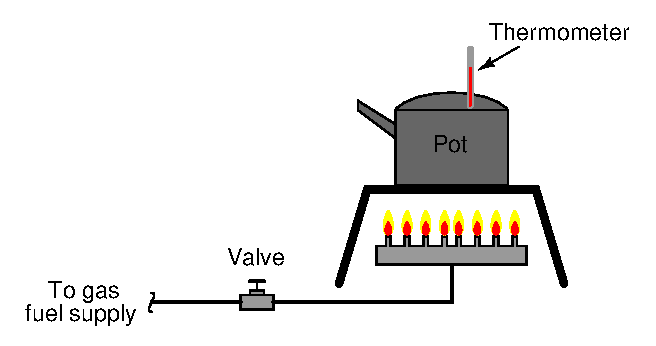
\includegraphics[width=1\columnwidth]{i01453x01.eps}$$

\vskip 30pt

\filbreak
\noindent
{\bf Example 2:} Level control application

$$\includegraphics[width=1\columnwidth]{i01453x02.eps}$$

\vskip 30pt

\filbreak
\noindent
{\bf Example 3:} Flow control application

$$\includegraphics[width=1\columnwidth]{i01453x03.eps}$$

\vskip 30pt

\filbreak
\noindent
{\bf Example 4:} Temperature control application

$$\includegraphics[width=1\columnwidth]{i01453x04.eps}$$
\end{multicols}
\vskip 20pt \vbox{\hrule \hbox{\strut \vrule{} {\bf Suggestions for Socratic discussion} \vrule} \hrule}

\begin{itemize}
\item{} Explain why ambient air temperature is considered a {\it load} to process example \#4, but the insulation thickness on the heat exchanger is not.
\end{itemize}

\underbar{file i01453}
\vfil \eject
%(END_QUESTION)





%(BEGIN_ANSWER)

A {\it load} is any variable in a process (besides the manipulated variable) that has influence over the process variable being controlled.

\vskip 10pt

Note: the following answers are not exhaustive.  In other words, there may be more loads than what is listed here for each process!

\begin{itemize}
\item{} Example 1: ambient air temperature
\item{} Example 2: incoming flow rate
\item{} Example 3: upstream and downstream pressures
\item{} Example 4: steam flow rate, steam temperature
\end{itemize}

%(END_ANSWER)





%(BEGIN_NOTES)

Students may be tempted to list process {\it constants} (such as vessel volume, heat exchanger tube thickness, etc.) as loads because they do impact the process dynamics.  However, the term ``load'' is typically reserved for some {\it variable} that has impact over the process, and is thus liable to change over time in such a way to challenge the loop controller.

To put this in different terms, the need to change setpoints, and the existence of variable loads in a process, both {\it justify} the presence of a controller.  If we were faced with a process never needing a different setpoint, and devoid of variable loads, there would be no need to place a control loop in it!  We could simply set a manually-actuated control valve where we wanted it to be, and leave it in that position forever!

\vfil \eject

\noindent
{\bf Prep Quiz:}

The definition of a {\it load} with regard to process control loops is:

\begin{itemize}
\item{} The time lag between a change in output and a change seen in the PV
\vskip 5pt 
\item{} The value at which the control system attempts to stabilize the PV over time
\vskip 5pt 
\item{} A device that dissipates energy in a circuit, as opposed to sourcing energy to the circuit
\vskip 5pt 
\item{} The multiplication factor of a process, measured from output to input
\vskip 5pt 
\item{} A drain of energy on a system, causing it to operate inefficiently
\vskip 5pt 
\item{} A variable affecting the PV, that is itself unregulated by the control system
\end{itemize}



%INDEX% Control, basics: load (definition)

%(END_NOTES)



%(BEGIN_QUESTION)
% Copyright 2006, Tony R. Kuphaldt, released under the Creative Commons Attribution License (v 1.0)
% This means you may do almost anything with this work of mine, so long as you give me proper credit

The following steam boiler is automated with a pneumatic water level transmitter, controller, and control valve.  This system ensures the water level in the steam drum remains approximately constant regardless of changes in steam demand or burner firing rate, and it is called a {\it single-element feedwater control} because it bases the feedwater valve position on a single variable (steam drum level):

$$\includegraphics[width=15.5cm]{i01461x01.eps}$$

The process variable (PV), setpoint (SP), and output signals (manipulated variable, or MV) of the controller are recorded in a table at random time intervals:

% No blank lines allowed between lines of an \halign structure!
% I use comments (%) instead, so that TeX doesn't choke.

$$\vbox{\offinterlineskip
\halign{\strut
\vrule \quad\hfil # \ \hfil & 
\vrule \quad\hfil # \ \hfil & 
\vrule \quad\hfil # \ \hfil \vrule \cr
\noalign{\hrule}
%
% First row
PV & SP & MV \cr
%
(Process Variable) & (Setpoint) & (Output) \cr
%
\noalign{\hrule}
%
% Another row
50\% & 50\% & 50\% \cr
%
\noalign{\hrule}
%
% Another row
48\% & 50\% & 70\% \cr
%
\noalign{\hrule}
%
% Another row
45\% & 50\% & 100\% \cr
%
\noalign{\hrule}
%
% Another row
49\% & 50\% & 60\% \cr
%
\noalign{\hrule}
%
% Another row
52\% & 50\% & 30\% \cr
%
\noalign{\hrule}
%
% Another row
51\% & 50\% & 40\% \cr
%
\noalign{\hrule}
%
% Another row
55\% & 50\% & 0\% \cr
%
\noalign{\hrule}
} % End of \halign 
}$$ % End of \vbox

Based on an examination of the values in this table, is the level controller configured for {\it direct} or {\it reverse} action?

\filbreak

Examining the controller, you notice there is a knob on its side for setting its gain.  This knob is labeled ``Gain / Prop. Band,'' and it has two sets of numbers describing its range of adjustment:

$$\includegraphics[width=15.5cm]{i01461x02.eps}$$

Explain how the two values shown for the knob's setting (Gain = 10 ; Prop. Band = 10\%) relate to the percentages you see in the table.  Particularly, define {\it proportional band} in a way that makes sense looking at the controller's behavior over time.

\vskip 20pt \vbox{\hrule \hbox{\strut \vrule{} {\bf Suggestions for Socratic discussion} \vrule} \hrule}

\begin{itemize}
\item{} Build a computer spreadsheet program to model the behavior of the proportional controller in this scenario.  You will know you are successful when it is able to duplicate the table of values presented in the question (i.e. your spreadsheet will be able to exactly calculate each Output value corresponding to the PV and SP values given in different rows of the table.
\end{itemize}

\underbar{file i01461}
%(END_QUESTION)





%(BEGIN_ANSWER)

This is a {\it reverse-acting} level controller: the output rises when the PV input falls, and vice-versa.

\vskip 10pt

``Proportional band'' is the percentage that the controller input (SP $-$ PV) must deviate in order to swing from 0\% to 100\% on the output.  As you may have noticed, proportional band is the mathematical reciprocal of gain.

%(END_ANSWER)





%(BEGIN_NOTES)



%INDEX% Control, proportional: gain versus proportional band
%INDEX% Control, proportional: proportional band versus gain
%INDEX% Process: steam boiler

%(END_NOTES)



%(BEGIN_QUESTION)
% Copyright 2006, Tony R. Kuphaldt, released under the Creative Commons Attribution License (v 1.0)
% This means you may do almost anything with this work of mine, so long as you give me proper credit

Convert the following controller gain settings into units of proportional band:
\begin{multicols}{2}
\begin{itemize}
\item{}Gain = 1; P.B. = \underbar{\hskip 50pt}
\vskip 5pt
\item{}Gain = 2; P.B. = \underbar{\hskip 50pt} 
\vskip 5pt
\item{}Gain = 3.0; P.B. = \underbar{\hskip 50pt} 
\vskip 5pt
\item{}Gain = 0.5; P.B. = \underbar{\hskip 50pt}
\vskip 5pt
\item{}Gain = 0.2; P.B. = \underbar{\hskip 50pt} 
\vskip 5pt
\item{}Gain = 0.01; P.B. = \underbar{\hskip 50pt} 
\vskip 5pt
\item{}Gain = 5.5; P.B. = \underbar{\hskip 50pt} 
\vskip 5pt
\item{}Gain = 10.2; P.B. = \underbar{\hskip 50pt} 
\end{itemize} 



\begin{itemize}
\item{}P.B. = 150\%; Gain = \underbar{\hskip 50pt}
\vskip 5pt
\item{}P.B. = 300\%; Gain = \underbar{\hskip 50pt} 
\vskip 5pt
\item{}P.B. = 40\%; Gain = \underbar{\hskip 50pt} 
\vskip 5pt
\item{}P.B. = 10\%; Gain = \underbar{\hskip 50pt} 
\vskip 5pt
\item{}P.B. = 730\%; Gain = \underbar{\hskip 50pt} 
\vskip 5pt
\item{}P.B. = 4\%; Gain = \underbar{\hskip 50pt} 
\vskip 5pt
\item{}P.B. = 247\%; Gain = \underbar{\hskip 50pt} 
\vskip 5pt
\item{}P.B. = 9.5\%; Gain = \underbar{\hskip 50pt} 
\end{itemize} 
\end{multicols}

\vskip 5pt 
Vis formel du bruker for utregningene. 
\vskip 5pt 
\underbar{file i01462}
\vfil \eject
%(END_QUESTION)





%(BEGIN_ANSWER)

\begin{itemize}
\item{}Gain = 1; P.B. = 100\%
\vskip 5pt
\item{}Gain = 2; P.B. = 50\%
\vskip 5pt
\item{}Gain = 3.0; P.B. = 33.3\%
\vskip 5pt
\item{}Gain = 0.5; P.B. = 200\%
\vskip 5pt
\item{}Gain = 0.2; P.B. = 500\%
\vskip 5pt
\item{}Gain = 0.01; P.B. = 10,000\%
\vskip 5pt
\item{}Gain = 5.5; P.B. = 18.18\%
\vskip 5pt
\item{}Gain = 10.2; P.B. = 9.804\%
\end{itemize} 



\begin{itemize}
\item{}P.B. = 150\%; Gain = 0.667
\vskip 5pt
\item{}P.B. = 300\%; Gain = 0.333
\vskip 5pt
\item{}P.B. = 40\%; Gain = 2.5
\vskip 5pt
\item{}P.B. = 10\%; Gain = 10
\vskip 5pt
\item{}P.B. = 730\%; Gain = 0.137
\vskip 5pt
\item{}P.B. = 4\%; Gain = 25
\vskip 5pt
\item{}P.B. = 247\%; Gain = 0.4049
\vskip 5pt
\item{}P.B. = 9.5\%; Gain = 10.53
\end{itemize} 

%(END_ANSWER)





%(BEGIN_NOTES)



%INDEX% Control, proportional: gain versus proportional band
%INDEX% Control, proportional: proportional band versus gain

%(END_NOTES)



%(BEGIN_QUESTION)
% Copyright 2006, Tony R. Kuphaldt, released under the Creative Commons Attribution License (v 1.0)
% This means you may do almost anything with this work of mine, so long as you give me proper credit

Convert the following controller settings (in units of proportional band) into units of gain (K$_{p}$):

\begin{itemize}
\item{}P.B. = 150\%; Gain = \underbar{\hskip 50pt}
\vskip 5pt
\item{}P.B. = 300\%; Gain = \underbar{\hskip 50pt} 
\vskip 5pt
\item{}P.B. = 40\%; Gain = \underbar{\hskip 50pt} 
\vskip 5pt
\item{}P.B. = 10\%; Gain = \underbar{\hskip 50pt} 
\vskip 5pt
\item{}P.B. = 730\%; Gain = \underbar{\hskip 50pt} 
\vskip 5pt
\item{}P.B. = 4\%; Gain = \underbar{\hskip 50pt} 
\vskip 5pt
\item{}P.B. = 247\%; Gain = \underbar{\hskip 50pt} 
\vskip 5pt
\item{}P.B. = 9.5\%; Gain = \underbar{\hskip 50pt} 
\end{itemize} 

\vskip 20pt \vbox{\hrule \hbox{\strut \vrule{} {\bf Suggestions for Socratic discussion} \vrule} \hrule}

\begin{itemize}
\item{} Demonstrate how to estimate answers for these conversions without using a calculator.
\end{itemize}

\underbar{file i01463}
%(END_QUESTION)





%(BEGIN_ANSWER)

\begin{itemize}
\item{}P.B. = 150\%; Gain = 0.667
\vskip 5pt
\item{}P.B. = 300\%; Gain = 0.333
\vskip 5pt
\item{}P.B. = 40\%; Gain = 2.5
\vskip 5pt
\item{}P.B. = 10\%; Gain = 10
\vskip 5pt
\item{}P.B. = 730\%; Gain = 0.137
\vskip 5pt
\item{}P.B. = 4\%; Gain = 25
\vskip 5pt
\item{}P.B. = 247\%; Gain = 0.4049
\vskip 5pt
\item{}P.B. = 9.5\%; Gain = 10.53
\end{itemize} 

%(END_ANSWER)





%(BEGIN_NOTES)



%INDEX% Control, proportional: gain versus proportional band
%INDEX% Control, proportional: proportional band versus gain

%(END_NOTES)



%(BEGIN_QUESTION)
% Copyright 2006, Tony R. Kuphaldt, released under the Creative Commons Attribution License (v 1.0)
% This means you may do almost anything with this work of mine, so long as you give me proper credit

Graph the output of this proportional-only controller, assuming a gain ($K_p$) value of 2.0, a bias value of 50\%, and a control action that is direct-acting:

$$\includegraphics[width=15.5cm]{i01468x01.eps}$$

\vskip 20pt \vbox{\hrule \hbox{\strut \vrule{} {\bf Suggestions for Socratic discussion} \vrule} \hrule}

\begin{itemize}
\item{} Explain why this trend graph of the PV is unrealistic for a real process, but nevertheless useful for learning how a proportional-only controller is designed to respond to changes in PV.
\item{} How do you suppose the PV would {\it actually} respond in a real process to the conditions shown (or implied) in this trend?  Sketch what you would think would be a more realistic response assuming a properly-tuned proportional-only controller running in automatic mode.
\end{itemize}

\underbar{file i01468}
%(END_QUESTION)





%(BEGIN_ANSWER)

$$\includegraphics[width=15.5cm]{i01468x02.eps}$$

%(END_ANSWER)





%(BEGIN_NOTES)


\vfil \eject

\noindent
{\bf Summary Quiz:}

The process controller generating the output seen on this trend is configured for:

$$\includegraphics[width=15.5cm]{i01468x03.eps}$$

\begin{itemize}
\item{} Direct control action
\vskip 5pt 
\item{} A proportional band value of 100\%
\vskip 5pt 
\item{} A gain value of 1.5
\vskip 5pt 
\item{} A proportional band value of 15\%
\vskip 5pt 
\item{} A gain value of 0.5
\vskip 5pt 
\item{} A proportional band value of 400\%
\end{itemize}



%INDEX% Control, proportional: graphing controller response

%(END_NOTES)



%(BEGIN_QUESTION)
% Copyright 2006, Tony R. Kuphaldt, released under the Creative Commons Attribution License (v 1.0)
% This means you may do almost anything with this work of mine, so long as you give me proper credit

Suppose that a reverse-acting, proportional-only controller has a gain ($K_p$) setting of 2 and a bias (b) setting of 40\%.  What will its output be for the following input conditions?

\begin{itemize}
\item{}PV = 37\%; SP = 50\%; Output = \underbar{\hskip 50pt}
\vskip 5pt
\item{}PV = 92\%; SP = 80\%; Output = \underbar{\hskip 50pt}
\vskip 5pt
\item{}PV = 81\%; SP = 75\%; Output = \underbar{\hskip 50pt}
\vskip 5pt
\item{}PV = 33\%; SP = 42\%; Output = \underbar{\hskip 50pt}
\vskip 5pt
\item{}PV = 79\%; SP = 76\%; Output = \underbar{\hskip 50pt}
\vskip 5pt
\item{}PV = 15\%; SP = 20\%; Output = \underbar{\hskip 50pt}
\vskip 5pt
\item{}PV = 38\%; SP = 38\%; Output = \underbar{\hskip 50pt}
\vskip 5pt
\item{}PV = 0\%; SP = 0\%; Output = \underbar{\hskip 50pt}
\end{itemize} 

\underbar{file i01489}
%(END_QUESTION)





%(BEGIN_ANSWER)

\begin{itemize}
\item{}PV = 37\%; SP = 50\%; Output = \underbar{\bf 66\%}
\vskip 5pt
\item{}PV = 92\%; SP = 80\%; Output = \underbar{\bf 16\%}
\vskip 5pt
\item{}PV = 81\%; SP = 75\%; Output = \underbar{\bf 28\%}
\vskip 5pt
\item{}PV = 33\%; SP = 42\%; Output = \underbar{\bf 58\%}
\vskip 5pt
\item{}PV = 79\%; SP = 76\%; Output = \underbar{\bf 34\%}
\vskip 5pt
\item{}PV = 15\%; SP = 20\%; Output = \underbar{\bf 50\%}
\vskip 5pt
\item{}PV = 38\%; SP = 38\%; Output = \underbar{\bf 40\%}
\vskip 5pt
\item{}PV = 0\%; SP = 0\%; Output = \underbar{\bf 40\%}
\end{itemize} 

%(END_ANSWER)





%(BEGIN_NOTES)



%INDEX% Control, proportional: calculating controller response

%(END_NOTES)



%(BEGIN_QUESTION)
% Copyright 2006, Tony R. Kuphaldt, released under the Creative Commons Attribution License (v 1.0)
% This means you may do almost anything with this work of mine, so long as you give me proper credit

A control valve (all by itself!) may act as a crude proportional controller for controlling pressure of a gas or vapor:

$$\includegraphics[width=15.5cm]{i01483x01.eps}$$

Identify how this constitutes a negative feedback system, and explain how it works to regulate downstream pressure.  Then, identify what things you would have to change in this system to alter its gain (proportional band) and setpoint.

\underbar{file i01483}
%(END_QUESTION)





%(BEGIN_ANSWER)

The principle is fairly straightforward to figure out, but gain and setpoint are not as easy.  To change gain, you could substitute a different-sized diaphragm in the valve actuator.  Setpoint adjustments could be made by changing the {\it bench set} of the valve.

%(END_ANSWER)





%(BEGIN_NOTES)

One could also alter gain by changing the spring in the actuator assembly with one having a different spring rate (the $k$ factor, as in Hooke's Law: $F = -kx$).

%INDEX% Control, proportional: control valve as crude proportional pressure controller

%(END_NOTES)



%(BEGIN_QUESTION)
% Copyright 2006, Tony R. Kuphaldt, released under the Creative Commons Attribution License (v 1.0)
% This means you may do almost anything with this work of mine, so long as you give me proper credit

A pneumatic water heater control system uses a temperature transmitter calibrated to a range of 0 to 180$^{o}$ F.  The control system has worked adequately for many years:

$$\includegraphics[width=15.5cm]{i01477x01.eps}$$

It is then decided that the temperature range is too wide, since the water temperature never falls below 100$^{o}$ F.  A narrower calibrated range will make better use of the 3-15 PSI signal's dynamic range, and also make it easier to see changes in temperature on 3-15 PSI (input) indicators and chart recorders.  An instrument technician re-calibrates the temperature transmitter to a narrower range: 100 to 180$^{o}$ F, then re-labels all the indicators and chart recorders to reflect the new range.  After doing this work, the operator places the control system back in service.

\filbreak

However, it quickly becomes evident that something is wrong.  Instead of a smooth line on the chart recorder, the temperature is seen to cycle continuously:

$$\includegraphics[width=15.5cm]{i01477x02.eps}$$

Why is this now happening, when the control used to be stable before the re-calibration?  Of course, we could fix the problem by returning the transmitter's calibration back to the way it was (0 to 180$^{o}$ F), but is there any way we can maintain the narrower transmitter range (100 to 180$^{o}$ F) {\it and} yet still have stable control, or are these two goals mutually exclusive?

\underbar{file i01477}
%(END_QUESTION)





%(BEGIN_ANSWER)

The problem is increased sensor gain with the new calibration range.  The solution is to reduce the controller's gain (increase its proportional band) to compensate.

%(END_ANSWER)





%(BEGIN_NOTES)



%INDEX% Control, proportional: effect of changing instrument calibration on process stability

%(END_NOTES)



%(BEGIN_QUESTION)
% Copyright 2006, Tony R. Kuphaldt, released under the Creative Commons Attribution License (v 1.0)
% This means you may do almost anything with this work of mine, so long as you give me proper credit

Some electronic controllers provide the option of a {\it time-proportioning} output instead of the customary {\it current-proportioning} output.  With the time-proportioning output, the two output terminals of the controller connect (internally) to a relay contact or transistor, capable only of turning an electrical load fully on and fully off:

$$\includegraphics[width=15.5cm]{i01487x01.eps}$$

Time-proportional control is most often used when the final control element is an electric heater.  Explain how time-proportional control works to maintain a process variable at setpoint while only being able to turn a heater on and off (and not in-between).

\underbar{file i01487}
%(END_QUESTION)





%(BEGIN_ANSWER)

The controller outputs a {\it Pulse-Width Modulated} signal, the duty cycle of the on/off cycling modulating energy input to the process through the heating element.

%(END_ANSWER)





%(BEGIN_NOTES)


%INDEX% Control, proportional: time-proportioning output

%(END_NOTES)



%(BEGIN_QUESTION)
% Copyright 2010, Tony R. Kuphaldt, released under the Creative Commons Attribution License (v 1.0)
% This means you may do almost anything with this work of mine, so long as you give me proper credit

Suppose you needed to control the temperature of an ``incubation'' vessel at a biopharmaceutical manufacturing facility, to ensure the bacteria were held at the correct temperature for optimum growth.  The vessel is heated by an electric heater, and the only controller you have available is one with a time-proportioning output (transistor).

Unfortunately, the controller's transistor is not able to directly handle the 240 volt AC power required by the heater, partly because of the voltage and current limitations of the transistor, and partly because an NPN transistor can only switch DC, not AC.

\vskip 50pt

$$\includegraphics[width=15.5cm]{i01488x01.eps}$$

\vskip 50pt

Sketch an ``interposing'' circuit between the controller and heating element that allows the controller to do its task.

\vfil 

\underbar{file i01488}
\eject
%(END_QUESTION)





%(BEGIN_ANSWER)

This is a graded question -- no answers or hints given!

%(END_ANSWER)





%(BEGIN_NOTES)

One of the most important general principles to keep in mind for this problem is the Law of Energy Conservation: {\it energy cannot be created or destroyed, but merely changed in form}.  Here, we are told the controller cannot handle either the voltage or the current necessary to energize a heating element.  This means no combination of passive components (capacitors, inductors, transformers, diodes, etc.) can ever boost the transistor's output power.  Instead, what the transistor can do is activate some kind of relay, which then switches 240 VAC power to the heating element.

Another important general principle to bear in mind is that transistors are not energy sources: one cannot simply connect the collector and emitter terminals of a transitor to a load device and expect that load device will receive power.  The transistor is merely an electronic {\it switch}: opening and closing to control direct current from some DC power source, which must be drawn in this circuit just like we need an AC power source to supply the heater.

Two alternative solutions are sketched here:

$$\includegraphics[width=15.5cm]{i01488x03.eps}$$

$$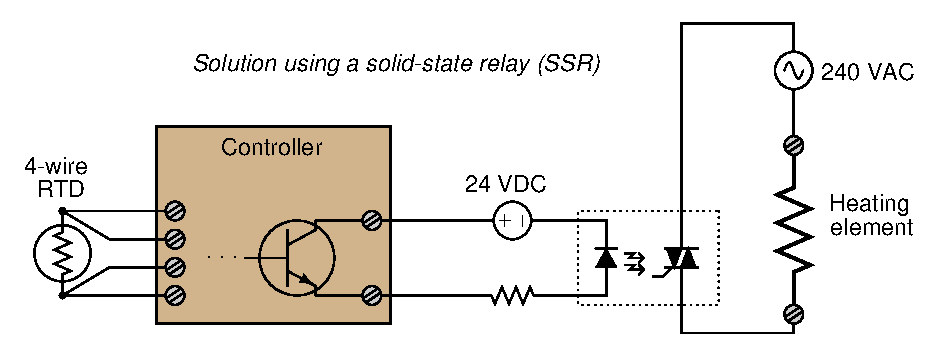
\includegraphics[width=15.5cm]{i01488x02.eps}$$

%INDEX% Control, proportional: time-proportioning output

%(END_NOTES)



%(BEGIN_QUESTION)
% Copyright 2006, Tony R. Kuphaldt, released under the Creative Commons Attribution License (v 1.0)
% This means you may do almost anything with this work of mine, so long as you give me proper credit

Her vises en P\&ID (Prosess og instrumenteringsdiagram) for en væskestrøm reguleringssløyfe. Den består av en strømningsmåler (FT) som registrer strømningen i røret og sender et elektronisk signal på for stor strømning det er. En strømingsregulator (FC) mottar signalet og sammenligner dette med et settpunkt, for så å avgjør hvilken vei reguleringsventilen skal bevege seg. En strøm til luft omformer (*(FY) konverterer strømsignalet fra regulatoren til et lufttrykk som styrer posisjonen til reguleringsventilen(FV), som igjen styrer strømningen i røret. 

$$\includegraphics[width=15.5cm]{i00124x01.eps}$$

Retningen på styresignalet for hvert instrument vises her:

\begin{itemize}
\item{} FT: Økende strømning = økende signal
\item{} FC: Økende signal på inngang (PV) = minkende signal på utgang (MV) 
\item{} FY: økende strømsignal på inngang = økende pneumatisk signal på utgangen 
\item{} FV: økende pneumatisk signal = ventilen åpner mer.
\end{itemize}

Forklar hva som  vil skje med alle signalene i denne reguleringssløyfen med regulatoren i "Auto" modus (Klar for å kompensere for variasjoner i strømningen) hvis pumpen plutselig roterer fortere og øsker strømningen. 

Forklar også hva som vil skje med styresignalene i reguleringssløyfen med regulatoren i "manual" modus(styresignalet står fast på det som operatøren har stilt det på) dersom pumpen roterer fortere og forårsaker en økning i strømningen. 


\vskip 20pt \vbox{\hrule \hbox{\strut \vrule{} {\bf Suggestions for Socratic discussion} \vrule} \hrule}

\begin{itemize}
\item{} Explain the practical benefit of having a ``manual'' mode in a process loop controller.  When might we intentionally use manual mode in an operating process condition?
\end{itemize}

\underbar{file i00124}
%(END_QUESTION)





%(BEGIN_ANSWER)

\noindent
{\bf In automatic mode:}

Process flow rate (increase) $\to$ FT output signal (increase milliamps) $\to$ FC output signal (decrease milliamps) $\to$ FY output signal (decrease PSI) $\to$ FV position (moves further closed, pinching off liquid flow).

\vskip 10pt

\noindent
{\bf In manual mode:}

Process flow rate (increase) $\to$ FT output signal (increase milliamps) $\to$ FC output signal (remains steady) $\to$ FY output signal (remains steady) $\to$ FV position (holds position).

\vskip 10pt

The important part of this question is the difference in response between ``automatic'' and ``manual'' controller modes.  In automatic control mode, the controller takes action to bring the process back to setpoint.  In manual control mode, the controller just lets the process drift and takes no action to stop it.

At first, having a ``manual'' mode in a control system seems pointless.  However, giving human operators the ability to manually override the otherwise automatic actions of a control system is important for start-up, shut-down, and handling emergency (unusual) conditions in a process system.  

Manual mode is also a very important diagnostic tool for instrument technicians and operators alike.  Being able to ``turn off the brain'' of an automatic control system and watch process response to manual changes in manipulated variable (final control element) signals gives technical personnel opportunity to test for unusual control valve behavior, process quirks, and other behaviors in a system that can lead to poor automatic control. 


%(END_ANSWER)





%(BEGIN_NOTES)




%INDEX% Control, basics: signal changes in an automatic control loop

%(END_NOTES)



%(BEGIN_QUESTION)
% Copyright 2006, Tony R. Kuphaldt, released under the Creative Commons Attribution License (v 1.0)
% This means you may do almost anything with this work of mine, so long as you give me proper credit

The very simplest style of automatic control is known as {\it on-off} or more whimsically, {\it bang-bang} control.  This is where the automatic controller only has two output signal modes: fully on and fully off.  Your home's heating system is most likely of this sort, where a thermostat can either tell the furnace to turn on or to turn off.

Describe the advantages and disadvantages of ``on-off'' control, as contrasted against more sophisticated control schemes where a final control element such as a control valve may be proportionately positioned anywhere between fully open and fully closed according to the demands of the process.

\vskip 20pt \vbox{\hrule \hbox{\strut \vrule{} {\bf Suggestions for Socratic discussion} \vrule} \hrule}

\begin{itemize}
\item{} What other control systems in common experience use the ``bang-bang'' strategy?
\end{itemize}

\underbar{file i00125}
%(END_QUESTION)





%(BEGIN_ANSWER)


%(END_ANSWER)





%(BEGIN_NOTES)

The main advantages of on/off control schemes is that they are simple and cheap.  The disadvantages include ``cycling'' of the final control element and also ``rippling'' of the process variable over time.  For rather obvious reasons, an on/off control system can never maintain a process variable at a steady value, but must always incur some up/down oscillation over time.

A common concept in on/off control systems is {\it hysteresis}, where the controller device turns on and off at different process variable points.  For example, consider a room heating system that starts the heater when the temperature falls below 70 degrees F, and does not turn the heater off until the temperature rises above 73 degrees F.  The three-degree difference between the on and off points is known as the {\it differential gap}, or {\it deadband} of the control system.  Normally we try to avoid having deadband within a process transmitter or control valve (since it makes steady control in a proportioning system nearly impossible).  However, some amount of deadband is usually a good thing to have in an on/off control system because it reduces the number of times the final control element must cycle over any given period of time.  Larger differential gaps mean fewer on/off cycles over time, but at the expense of greater up-and-down oscillations in process variable.

%INDEX% Control, basics: on/off control

%(END_NOTES)



%(BEGIN_QUESTION)
% Copyright 2011, Tony R. Kuphaldt, released under the Creative Commons Attribution License (v 1.0)
% This means you may do almost anything with this work of mine, so long as you give me proper credit

An indispensible tool for process operators and instrument technicians alike is the {\it trend} graph, showing such control loop variables as PV, SP, and controller Output superimposed on the same time-domain plot.  The following example shows the process variable, setpoint, and output for a proportional-only controller as it responds to changes in a control loop's PV while the setpoint remains at a constant value of 40\%:

$$\includegraphics[width=15.5cm]{i00715x01.eps}$$

Based on an examination of this trend graph, determine the {\it bias} value of the controller and {\it gain} value of the controller, as well as its direction of action ({\it direct} or {\it reverse}).  

\vskip 10pt

A helpful analysis technique when relating trend graphs to controller equations is to sketch a vertical line on the graph to identify some particular point in time, then identify the values of PV, SP, and Output at that point in time.  A proper equation for the controller will successfully predict the Output value from the PV and SP values at {\it any} point in time shown on the trend.

\vskip 20pt \vbox{\hrule \hbox{\strut \vrule{} {\bf Suggestions for Socratic discussion} \vrule} \hrule}

\begin{itemize}
\item{} Once you have calculated the gain of this loop controller, calculate its {\it proportional band} value as well.
\item{} Build a computer spreadsheet program to model the behavior of the proportional controller in this scenario.  You will know you are successful when it is able to duplicate any Output value shown on the trend graph at any particular point in time, corresponding to the PV and SP values at that same point in time.
\item{} What would this trend look like if the controller were left in {\it manual} mode instead of {\it automatic} mode?
\end{itemize}

\underbar{file i00715}
%(END_QUESTION)





%(BEGIN_ANSWER)

Gain = 0.5 and bias = 30\%

%(END_ANSWER)





%(BEGIN_NOTES)

The gain may be calculated by comparing output change ($\Delta m$) with input change ($\Delta$PV) between any two points in time on the trend.  Bias is most easily determined by noting the output value when the error is equal to zero (PV = SP).

%INDEX% Control, proportional: graphing controller response

%(END_NOTES)



%(BEGIN_QUESTION)
% Copyright 2006, Tony R. Kuphaldt, released under the Creative Commons Attribution License (v 1.0)
% This means you may do almost anything with this work of mine, so long as you give me proper credit

A {\it microcontroller} is a single-chip digital computer with onboard I/O capable of receiving and transmitting different types of electrical signals, and a processor capable of executing a series of written instructions.  This one is being used to control an air compressor:

$$\includegraphics[width=15.5cm]{i01454x01.eps}$$

Examine the following program (written in an informal programming language called ``pseudocode'') and explain how the microcontroller decides when to turn the motor on and off.  Also determine the pressures at which the microcontroller turns on and shuts off the compressor:

\vskip 10pt

\hbox{ \vrule
\vbox{ \hrule \vskip 3pt
\hbox{ \hskip 3pt
\vbox{ \hsize=5in \raggedright

\noindent
\underbar{\bf Pseudocode listing}

\vskip 10pt

{\tt Declare Pin0 as an analog input (scale 0 to 5 volts = 0 to 1023)}

{\tt Declare Pin1 as a discrete output}

{\tt Declare Pin2 as a discrete output}

{\tt Declare A as a constant = 805}

{\tt Declare B as a constant = 750}

{\tt Declare C as a constant = 700}

\vskip 10pt

{\tt LOOP}

\hskip 10pt {\it // (Comment: Motor control points)}

\hskip 10pt {\tt IF Pin0 > A, SET Pin1 LOW}

\hskip 10pt {\tt ELSEIF Pin0 < B, SET Pin1 HIGH}

\hskip 10pt {\tt ENDIF}

\vskip 10pt

\hskip 10pt {\it // (Comment: Alarm LED control points)}

\hskip 10pt {\tt IF Pin0 < C, SET Pin2 HIGH}

\hskip 10pt {\tt ELSE SET Pin2 LOW}

\hskip 10pt {\tt ENDIF}

{\tt ENDLOOP}
}
\hskip 3pt}%
\vskip 5pt \hrule}%
\vrule}

\vskip 20pt \vbox{\hrule \hbox{\strut \vrule{} {\bf Suggestions for Socratic discussion} \vrule} \hrule}

\begin{itemize}
\item{} Which sections of the pseudocode program listing are executed repeatedly, and which sections are executed only once?
\item{} How many bits of resolution does this microcontroller have for the analog input on pin \#0, assuming that 0 to 1023 is the full range of the converter?
\item{} Explain how the {\it solid state relay} device works to help control the compressor motor.
\item{} Explain what would happen if you deleted the {\tt LOOP} and {\tt ENDLOOP} statements in the microcontroller program.
\item{} Modify the pseudocode so that the alarm LED comes on if the pressure gets too high.
\item{} Modify the pseudocode so that the alarm LED comes on if the pressure gets too high {\it or} too low.
\end{itemize}

\underbar{file i01454}
%(END_QUESTION)





%(BEGIN_ANSWER)

{\tt A} = {\tt 805} = 110 PSI (motor stop point)

{\tt B} = {\tt 750} = 100 PSI (motor start point)

{\tt C} = {\tt 700} = 90.8 PSI (low air pressure alarm point)

%(END_ANSWER)





%(BEGIN_NOTES)

The pressure transmitter measures 0 to 150 PSI and outputs 4 to 20 mA.  That current, passing through a 250 ohm resistor, creates a 1 to 5 volt signal for the microcontroller's ADC to read (as a numerical count value ranging as high as 1023 counts).

\vskip 10pt

The LRV (1 volt) generates a count value of 205 counts ($1 \over 5$ of 1023).  Therefore, 205 to 1023 represents 0 to 150 PSI.  The count values specified in the program correspond to the following pressures:

\begin{itemize}
\item{} $A$ = 805 counts = ${805 \over 1023} \times 5$ = 3.9345 volts = 110.04 PSI
\vskip 5pt
\item{} $B$ = 750 counts = ${750 \over 1023} \times 5$ = 3.6657 volts = 99.96 PSI
\vskip 5pt
\item{} $C$ = 700 counts = ${700 \over 1023} \times 5$ = 3.4213 volts = 90.80 PSI
\end{itemize}

The compressor motor stops when the pressure exceeds $A$ (110.04 PSI), and re-starts when it falls below $B$ (99.96 PSI).  An alarm bit is set if the pressure is less than $C$ (90.80 PSI).

\vskip 10pt

$2^{10} = 1024$, so this must be a 10-bit ADC.









\vskip 20pt \vbox{\hrule \hbox{\strut \vrule{} {\bf Virtual Troubleshooting} \vrule} \hrule}

This question is a good candidate for a ``Virtual Troubleshooting'' exercise.  Presenting the diagram to students, you first imagine in your own mind a particular fault in the system.  Then, you present one or more symptoms of that fault (something noticeable by an operator or other user of the system).  Students then propose various diagnostic tests to perform on this system to identify the nature and location of the fault, as though they were technicians trying to troubleshoot the problem.  Your job is to tell them what the result(s) would be for each of the proposed diagnostic tests, documenting those results where all the students can see.

During and after the exercise, it is good to ask students follow-up questions such as:

\begin{itemize}
\item{} What does the result of the last diagnostic test tell you about the fault?
\item{} Suppose the results of the last diagnostic test were different.  What then would that result tell you about the fault?
\item{} Is the last diagnostic test the best one we could do?
\item{} What would be the ideal order of tests, to diagnose the problem in as few steps as possible?
\end{itemize}

%INDEX% Control, basics: on/off control (implemented in a microcontroller)

%(END_NOTES)



%(BEGIN_QUESTION)
% Copyright 2006, Tony R. Kuphaldt, released under the Creative Commons Attribution License (v 1.0)
% This means you may do almost anything with this work of mine, so long as you give me proper credit

Imagine driving an automobile with very sensitive steering: just a few degrees of steering wheel motion at highway speeds is sufficient to quickly change lanes.  Now imagine driving an automobile having significantly less sensitive steering: a whole quarter-turn of the steering wheel is needed to generate the same response as a few degrees of rotation in the first vehicle.

An important process quantity is its {\it gain}.  How would you qualify the two automobile steering systems just described in terms of process gain, from the perspective of lane position as the process variable, steering wheel angle as the manipulated variable, and you (the driver) as the proportional controller?  Which automobile has a high process gain, and which has a low process gain?

\underbar{file i01457}
%(END_QUESTION)





%(BEGIN_ANSWER)

The automobile with ``sensitive'' steering has the greater process gain.  As always, the ``gain'' of a system is a ratio of its output change to its input change ($\Delta \hbox{Out} \over \Delta \hbox{In}$, or $d \hbox{Out} \over d \hbox{In}$), and process gain is no exception.

%(END_ANSWER)





%(BEGIN_NOTES)


%INDEX% Control, proportional: process gain

%(END_NOTES)



%(BEGIN_QUESTION)
% Copyright 2006, Tony R. Kuphaldt, released under the Creative Commons Attribution License (v 1.0)
% This means you may do almost anything with this work of mine, so long as you give me proper credit

Examine this flow control system, where a valve controls the flow rate of liquid between two vessels:

$$\includegraphics[width=15.5cm]{i01458x01.eps}$$

Since each vessel has its liquid level controlled by an overflow pipe, the head pressure at the bottom of each will be constant.  This means that the differential pressure across the valve will be constant as well.

\vskip 10pt

Suppose now that the higher vessel has its overflow pipe moved to a lower location, thus reducing the controlled level in that vessel, and consequently the head pressure generated at the bottom:

$$\includegraphics[width=15.5cm]{i01458x02.eps}$$
 
This change in head pressure, of course, reduces the amount of differential pressure across the valve.  How will this affect the process gain, as it relates to flow control?  In other words, will the flow rate become more or less sensitive to changes in valve position as a result of decreasing the pressure drop across the valve?

\vskip 10pt

What will happen to the process gain if we then replace the control valve with one having a larger $C_v$ value (a larger opening for fluid flow when fully open)?

\vskip 10pt

Finally, what will happen to the process gain if we re-calibrated the flow transmitter for a smaller span (for example, from 0-120 GPM to 0-75 GPM)?

\underbar{file i01458}
%(END_QUESTION)





%(BEGIN_ANSWER)

Reducing the differential pressure drop across the valve will result in less flow when the valve is fully open.  Of course, the flow rate will still be zero when the valve is fully closed.  This means that the controllable flow {\it range} has been decreased as a result of decreased pressure drop across the valve.

With less of a controllable flow range, the flow will not change as much as it did before given the same change in valve position.  That is to say, the process variable in this control system will be less sensitive to changes in valve position than before.  In other words, we are faced with a {\it decreased} process gain.

\vskip 10pt

Given a larger valve, the process gain will {\it increase}, because greater changes in flow rate will result from the same changes in valve position with a valve of greater size.

Technically speaking, the gain of the valve (ratio of valve coefficient, or C$_{v}$, versus position change) is a separate variable from the gain of the process itself (ratio of flow rate versus valve coefficient), and this is separate from the gain of the sensor (ratio of transmitter output percentage versus flow rate).  However, here I use the term ``process gain'' to refer to the sensitivity of the whole control system, except the controller (the process vessels and piping, control valve, and flow transmitter).

\vskip 10pt

Given a flow transmitter with a smaller range, the process gain will {\it increase}, because the same changes in valve position will now result in greater {\it percentage} changes in the transmitter output.

%(END_ANSWER)





%(BEGIN_NOTES)


%INDEX% Control, proportional: process gain

%(END_NOTES)



%(BEGIN_QUESTION)
% Copyright 2006, Tony R. Kuphaldt, released under the Creative Commons Attribution License (v 1.0)
% This means you may do almost anything with this work of mine, so long as you give me proper credit

In your study of electronics, you probably learned that any amplifier can be turned into an {\it oscillator} by providing the right amount of phase-shifted feedback from output to input, with a minimum amount of total circuit gain.  This principle even had a name: the {\it Barkhausen criterion}.

$$\includegraphics[width=15.5cm]{i01459x01.eps}$$

So long as the product of the two gains is at least unity ($A_{amp} \cdot A_{feedback} \geq 1$), there will be sufficient amplification to sustain oscillation in the circuit.  One key to avoiding oscillation in such a circuit is to limit the total ``loop'' gain to less than unity.

\vskip 10pt

A process control system using feedback is not much different from this, and it too may oscillate if the total ``loop'' gain is excessive:

$$\includegraphics[width=15.5cm]{i01459x02.eps}$$

Describe what ``gain'' represents in each of the four components within the control system shown above ($A_C$, $A_{fce}$, $A_{process}$, and $A_T$), and identify which of these gains is easiest to alter.  Finally, explain how that one (easy-to-set) gain should be adjusted.  In other words, what criteria should determine its configured value?

\underbar{file i01459}
%(END_QUESTION)





%(BEGIN_ANSWER)

For each component in the control system, ``gain'' is defined in the same terms that gain is defined for any electronic component -- the ratio of output change to input change:

$$\hbox{Gain } = {\Delta \hbox{Out} \over \Delta \hbox{In}}$$

We may be more precise in our definition if we use calculus notation and express this ratio as a {\it derivative}:

$$\hbox{Gain } = {d \hbox{Out} \over d \hbox{In}}$$

As for how and why to set the controller gain at a particular value, I will let you discuss this with your classmates and arrive at your own answer!  I will say this, though: we do {\it not} want the system to break into oscillations!

\vskip 10pt

Challenge question: as you may (should!) recall, a necessary condition for oscillation in a feedback system is that the feedback be {\it positive}.  In other words, the phase shift from amplifier output to amplifier input needs to be 360$^{o}$, or else any oscillation will quickly die out due to interference, regardless of gain.  This being said, how can a control system ever oscillate, because we know the feedback is normally {\it negative} in nature, not positive?  Even if the controller gain were huge, shouldn't the inherently negative feedback of the system naturally prevent oscillation?

%(END_ANSWER)





%(BEGIN_NOTES)

Controller gain is obviously the easiest gain to set in a control system, and it should be set at a value great enough to provide quick, responsive control; but not so great that it causes the system to become unstable and oscillate.

\vskip 10pt

It is illustrative to have students generate the following gain equations for each of the four components shown in the process control loop (transmitter, controller, valve, and process):

$$\hbox{Transmitter Gain } = {\Delta \hbox{PV signal} \over \Delta \hbox{Measured variable}}$$

$$\hbox{Controller Gain } = {\Delta \hbox{MV signal} \over \Delta \hbox{PV signal}}$$

$$\hbox{Valve Gain } = {\Delta C_v \over \Delta \hbox{MV signal}}$$

$$\hbox{Process Gain } = {\hbox{Measured variable} \over \Delta C_v}$$

Note how the input of the next instrument in the loop comes from the output of the last!  This progression clearly shows the ``chain'' of information from one element to the other.

\vskip 10pt

In answer to the challenge question, negative feedback certainly would prohibit oscillation regardless of gain.  However, there will {\it always} be time lags in a feedback system, which mean that oscillation frequencies will be phase-shifted by those time lags.  At some frequency, every control system will develop an additional 180$^{o}$ of phase shift between controller output and controller input, thus turning what was originally negative feedback into positive feedback.  This, incidentally, is why feedback systems seek certain particular frequencies to oscillate at!  All other frequencies fail to generate the necessary phase shift for regenerative feedback, and thus die out.

%INDEX% Control, proportional: loop gain
%INDEX% Electronics review: Barkhausen criterion

%(END_NOTES)



%(BEGIN_QUESTION)
% Copyright 2006, Tony R. Kuphaldt, released under the Creative Commons Attribution License (v 1.0)
% This means you may do almost anything with this work of mine, so long as you give me proper credit

The following water heater process is automated with a pneumatic temperature transmitter, controller, and control valve:

$$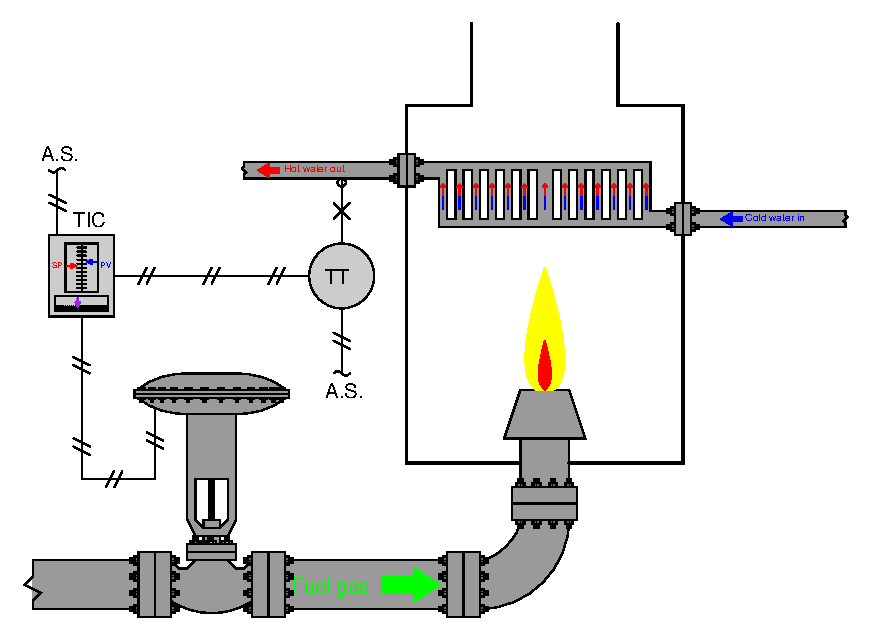
\includegraphics[width=15.5cm]{i01460x01.eps}$$

The process variable (PV), setpoint (SP), and output signals (manipulated variable, or MV) of the controller are recorded in a table at random time intervals:

% No blank lines allowed between lines of an \halign structure!
% I use comments (%) instead, so that TeX doesn't choke.

$$\vbox{\offinterlineskip
\halign{\strut
\vrule \quad\hfil # \ \hfil & 
\vrule \quad\hfil # \ \hfil & 
\vrule \quad\hfil # \ \hfil \vrule \cr
\noalign{\hrule}
%
% First row
PV & SP & MV \cr
%
(Process Variable) & (Setpoint) & (Output) \cr
%
\noalign{\hrule}
%
% Another row
50\% & 50\% & 50\% \cr
%
\noalign{\hrule}
%
% Another row
45\% & 50\% & 55\% \cr
%
\noalign{\hrule}
%
% Another row
30\% & 50\% & 70\% \cr
%
\noalign{\hrule}
%
% Another row
25\% & 50\% & 75\% \cr
%
\noalign{\hrule}
%
% Another row
65\% & 50\% & 35\% \cr
%
\noalign{\hrule}
%
% Another row
72\% & 50\% & 28\% \cr
%
\noalign{\hrule}
%
% Another row
50\% & 40\% & 40\% \cr
%
\noalign{\hrule}
%
% Another row
50\% & 71\% & 71\% \cr
%
\noalign{\hrule}
%
% Another row
80\% & 65\% & 35\% \cr
%
\noalign{\hrule}
%
% Another row
37\% & 42\% & 55\% \cr
%
\noalign{\hrule}
%
% Another row
40\% & 30\% & 40\% \cr
%
\noalign{\hrule}
} % End of \halign 
}$$ % End of \vbox

Develop a mathematical expression describing the data you see here in the table.  Hint: it may be easier if you begin with a {\it qualitative} assessment of the figures (i.e. {\it ``when the PV exceeds the SP, the MV . . .''}).

\underbar{file i01460}
%(END_QUESTION)





%(BEGIN_ANSWER)

MV = SP $-$ PV + 50\%

%(END_ANSWER)





%(BEGIN_NOTES)


%INDEX% Control, proportional: controller gain

%(END_NOTES)



%(BEGIN_QUESTION)
% Copyright 2006, Tony R. Kuphaldt, released under the Creative Commons Attribution License (v 1.0)
% This means you may do almost anything with this work of mine, so long as you give me proper credit

{\it Digital} proportional controllers generate their output signal values using a microprocessor to repeatedly evaluate the proportional equation:

$$m = K_p e + b$$
 
What would happen if a {\it negative} value were entered for gain ($K_p$) into the digital controller's program?

\underbar{file i01467}
%(END_QUESTION)





%(BEGIN_ANSWER)

The effect of a negative $K_p$ value in a digital controller's algorithm would be to reverse the control action (from reverse-acting to direct-acting, or from direct-acting to reverse-acting), because a positive error would {\it decrease} the output, and vice-versa.  This is assuming, of course, that the controller is programmed to accept such values.  A wise programmer might make it impossible to enter negative tuning constant values, to avoid confusion from someone accidently entering one and unintentionally reversing the control action.

%(END_ANSWER)





%(BEGIN_NOTES)


%INDEX% Control, proportional: digital electronic controller

%(END_NOTES)



%(BEGIN_QUESTION)
% Copyright 2006, Tony R. Kuphaldt, released under the Creative Commons Attribution License (v 1.0)
% This means you may do almost anything with this work of mine, so long as you give me proper credit

Tegn grafen for utgangen  på denne regulatoren med bare p-ledd og direktevirkning. Den er stilt inn med følgende verdier:
\begin{itemize}[noitemsep]
	\item proporsjonalbånd 20\%
	\item bias 50 \%
\end{itemize}

%Graph the output of this proportional-only controller, assuming a proportional band value of 20\%, a bias value of 50\%, and a control action that is direct-acting:

$$\includegraphics[width=15.5cm]{i01469x01.eps}$$
Utregninger:\\

\begin{tikzpicture}
	\draw[step=0.5cm,gray!20,very thin]  grid (16,6) ;
\end{tikzpicture}
\vskip 20pt \vbox{\hrule \hbox{\strut \vrule{} {\bf Suggestions for Socratic discussion} \vrule} \hrule}

\begin{itemize}
\item{} Explain why this trend graph of the PV is unrealistic for a real process, but nevertheless useful for learning how a proportional-only controller is designed to respond to changes in PV.
\item{} How do you suppose the PV would {\it actually} respond in a real process to the conditions shown (or implied) in this trend?  Sketch what you would think would be a more realistic response assuming a properly-tuned proportional-only controller running in automatic mode.
\item{} Identify points on the trend where the PV exhibits a positive rate of change. 
\item{} Identify points on the trend where the PV exhibits a negative rate of change. 
\item{} Identify points on the trend where the PV exhibits zero change. 
\end{itemize}

\underbar{file i01469}
%(END_QUESTION)





%(BEGIN_ANSWER)

$$\includegraphics[width=15.5cm]{i01469x02.eps}$$

%(END_ANSWER)





%(BEGIN_NOTES)

With a proportional band value of 20\%, the gain will be equal to 5.

%INDEX% Control, proportional: graphing controller response

%(END_NOTES)



%(BEGIN_QUESTION)
% Copyright 2006, Tony R. Kuphaldt, released under the Creative Commons Attribution License (v 1.0)
% This means you may do almost anything with this work of mine, so long as you give me proper credit

Graph the output of this proportional-only controller, assuming a proportional band value of 125\%, a bias value of 30\%, and a control action that is reverse-acting:

$$\includegraphics[width=15.5cm]{i01470x01.eps}$$

\vskip 20pt \vbox{\hrule \hbox{\strut \vrule{} {\bf Suggestions for Socratic discussion} \vrule} \hrule}

\begin{itemize}
\item{} Identify points on the trend where the PV exhibits a positive rate of change. 
\item{} Identify points on the trend where the PV exhibits a negative rate of change. 
\item{} Identify points on the trend where the PV exhibits zero change. 
\item{} How would the output signal trend be altered if the {\it gain} of this controller were increased?
\item{} How would the output signal trend be altered if the {\it bias} of this controller were increased?
\item{} How would the output signal trend be altered if the {\it action} of this controller were switched from reverse to direct?
\end{itemize}

\underbar{file i01470}
%(END_QUESTION)





%(BEGIN_ANSWER)

$$\includegraphics[width=15.5cm]{i01470x02.eps}$$

With a proportional band value of 125\%, the gain will be equal to 0.8.

$$m = 0.8(\hbox{SP} - \hbox{PV}) + 30$$

% No blank lines allowed between lines of an \halign structure!
% I use comments (%) instead, so that TeX doesn't choke.

$$\vbox{\offinterlineskip
\halign{\strut
\vrule \quad\hfil # \ \hfil & 
\vrule \quad\hfil # \ \hfil & 
\vrule \quad\hfil # \ \hfil \vrule \cr
\noalign{\hrule}
%
% First row
{\bf PV} & {\bf SP} & {\bf Output} \cr
%
\noalign{\hrule}
%
% Another row
65\% & 70\% & 34\% \cr
%
\noalign{\hrule}
%
% Another row
50\% & 70\% & 46\% \cr
%
\noalign{\hrule}
%
% Another row
60\% & 70\% & 38\% \cr
%
\noalign{\hrule}
} % End of \halign 
}$$ % End of \vbox


%(END_ANSWER)





%(BEGIN_NOTES)


%INDEX% Control, proportional: graphing controller response

%(END_NOTES)



%(BEGIN_QUESTION)
% Copyright 2006, Tony R. Kuphaldt, released under the Creative Commons Attribution License (v 1.0)
% This means you may do almost anything with this work of mine, so long as you give me proper credit

Graph the output of this proportional-only controller, assuming a proportional band value of 100\% and a control action that is direct-acting:

$$\includegraphics[width=15.5cm]{i01484x01.eps}$$

\underbar{file i01484}
%(END_QUESTION)





%(BEGIN_ANSWER)

$$\includegraphics[width=15.5cm]{i01484x02.eps}$$

%(END_ANSWER)





%(BEGIN_NOTES)

With a proportional band value of 100\%, the gain will be equal to 1.

%INDEX% Control, proportional: graphing controller response

%(END_NOTES)



%(BEGIN_QUESTION)
% Copyright 2006, Tony R. Kuphaldt, released under the Creative Commons Attribution License (v 1.0)
% This means you may do almost anything with this work of mine, so long as you give me proper credit

Graph the output of this proportional-only controller, assuming a gain ($K_p$) value of 0.5, a bias value of 40\%, and a control action that is reverse-acting:

$$\includegraphics[width=15.5cm]{i01485x01.eps}$$

\vskip 20pt \vbox{\hrule \hbox{\strut \vrule{} {\bf Suggestions for Socratic discussion} \vrule} \hrule}

\begin{itemize}
\item{} Identify points on the trend where the PV exhibits a positive rate of change. 
\item{} Identify points on the trend where the PV exhibits a negative rate of change. 
\item{} Identify points on the trend where the PV exhibits zero change. 
\item{} How would the output signal trend be altered if the {\it gain} of this controller were decreased?
\item{} How would the output signal trend be altered if the {\it bias} of this controller were decreased?
\item{} How would the output signal trend be altered if the {\it action} of this controller were switched from reverse to direct?
\end{itemize}

\underbar{file i01485}
%(END_QUESTION)





%(BEGIN_ANSWER)

$$\includegraphics[width=15.5cm]{i01485x02.eps}$$

%(END_ANSWER)





%(BEGIN_NOTES)

With a gain of 0.5, the proportional band value will be 200\%.

$$m = 0.5(\hbox{SP} - \hbox{PV}) + 40$$

% No blank lines allowed between lines of an \halign structure!
% I use comments (%) instead, so that TeX doesn't choke.

$$\vbox{\offinterlineskip
\halign{\strut
\vrule \quad\hfil # \ \hfil & 
\vrule \quad\hfil # \ \hfil & 
\vrule \quad\hfil # \ \hfil \vrule \cr
\noalign{\hrule}
%
% First row
{\bf PV} & {\bf SP} & {\bf Output} \cr
%
\noalign{\hrule}
%
% Another row
50\% & 45\% & 37.5\% \cr
%
\noalign{\hrule}
%
% Another row
70\% & 45\% & 27.5\% \cr
%
\noalign{\hrule}
%
% Another row
70\% & 55\% & 32.5\% \cr
%
\noalign{\hrule}
%
% Another row
50\% & 40\% & 35\% \cr
%
\noalign{\hrule}
} % End of \halign 
}$$ % End of \vbox


%INDEX% Control, proportional: graphing controller response

%(END_NOTES)



%(BEGIN_QUESTION)
% Copyright 2006, Tony R. Kuphaldt, released under the Creative Commons Attribution License (v 1.0)
% This means you may do almost anything with this work of mine, so long as you give me proper credit

Examine this microcontroller circuit and program, designed to act as a general-purpose proportional controller:

$$\includegraphics[width=15.5cm]{i01486x01.eps}$$

\hbox{ \vrule
\vbox{ \hrule \vskip 3pt
\hbox{ \hskip 3pt
\vbox{ \hsize=5in \raggedright

\noindent
\underbar{\bf Pseudocode listing}

\vskip 10pt

{\tt Declare Pin0 as an analog input (scale 0 to 5 volts = 0 to 1023)}

{\tt Declare Pin1 as an analog output (scale 0 to 5 volts = 0 to 1023)}

{\tt Declare SP as a variable, initially set to a value of 614}

{\tt Declare GAIN as a variable, initially set to a value of 1.0}

{\tt Declare ERROR as a variable}

{\tt Declare BIAS as a constant = 614}

\vskip 10pt

{\tt LOOP}

\hskip 10pt {\tt SET ERROR = Pin0 - SP}

\hskip 10pt {\tt SET Pin1 = (GAIN * ERROR) + BIAS}

{\tt ENDLOOP}
}
\hskip 3pt}%
\vskip 5pt \hrule}%
\vrule}


\vskip 10pt

Is this controller {\it direct} or {\it reverse} acting?  What edit(s) to the program listing would be required to change the direction of the controller's action?  

\vskip 20pt \vbox{\hrule \hbox{\strut \vrule{} {\bf Suggestions for Socratic discussion} \vrule} \hrule}

\begin{itemize}
\item{} Which sections of the pseudocode program listing are executed repeatedly, and which sections are executed only once?
\item{} How many bits of resolution does this microcontroller have for the analog input on pin \#1, assuming that 0 to 1023 is the full range of the converter?
\item{} Does the speed of program execution (i.e. how fast the loop repeats itself) affect the controller's ability to control a process?
\item{} Could all the ``Declare'' instructions be placed within the loop of this program?  Why or why not?
\item{} Explain what would happen if you deleted the {\tt LOOP} and {\tt ENDLOOP} statements in the microcontroller program.
\item{} Modify this program to include a PV alarm, turning on an LED alarm lamp if the PV exceeds a certain value, and turning it back off when the PV drops below another value.
\end{itemize}


\underbar{file i01486}
%(END_QUESTION)





%(BEGIN_ANSWER)

The controller code as shown implements {\it direct} action, since the error is calculated as PV $-$ SP.

\vskip 10pt

The following additions give this controller the ability to switch between direct or reverse control action:

$$\includegraphics[width=15.5cm]{i01486x02.eps}$$

\hbox{ \vrule
\vbox{ \hrule \vskip 3pt
\hbox{ \hskip 3pt
\vbox{ \hsize=5in \raggedright

\noindent
\underbar{\bf Pseudocode listing}

\vskip 10pt

{\tt Declare Pin0 as an analog input (scale 0 to 5 volts = 0 to 1023)}

{\tt Declare Pin1 as an analog output (scale 0 to 5 volts = 0 to 1023)}

{\tt Declare Pin7 as a discrete input}

{\tt Declare SP as a variable, initially set to a value of 614}

{\tt Declare GAIN as a variable, initially set to a value of 1.0}

{\tt Declare ERROR as a variable}

{\tt Declare BIAS as a constant = 614}

\vskip 10pt

{\tt LOOP}

\hskip 10pt {\tt IF Pin7 = 0, SET ERROR = Pin0 - SP }

\hskip 10pt {\tt ELSE, SET ERROR = SP - Pin0}

\hskip 10pt {\tt ENDIF}

\vskip 10pt

\hskip 10pt {\tt SET Pin1 = (GAIN * ERROR) + BIAS}

{\tt ENDLOOP}
}
\hskip 3pt}%
\vskip 5pt \hrule}%
\vrule}


\vskip 10pt

While a very slow program execution time could be bad for control, it actually could serve a useful purpose in some processes.  In processes with large dead times (transport delays), one control strategy to apply is called {\it sample-and-hold}, which is precisely what this program would be if a purposeful and substantial delay time were inserted into the loop.

%(END_ANSWER)





%(BEGIN_NOTES)

\vfil \eject

\noindent
{\bf Summary Quiz:}

Determine whether this digital control program is {\it direct-acting} or {\it reverse-acting}:

\vskip 10pt

\hbox{ \vrule
\vbox{ \hrule \vskip 3pt
\hbox{ \hskip 3pt
\vbox{ \hsize=5in \raggedright

\noindent
\underbar{\bf Pseudocode listing}

\vskip 10pt

{\tt Declare Pin0 as an analog input (scale 0 to 5 volts = 0 to 1023)} {\it (PV)}

{\tt Declare Pin1 as an analog output (scale 0 to 5 volts = 0 to 1023)}

{\tt Declare SP as a variable, initially set to a value of 512}

{\tt Declare GAIN as a variable, initially set to a value of 1.0}

{\tt Declare ERROR as a variable}

{\tt Declare BIAS as a constant = 512}

\vskip 10pt

{\tt LOOP}

\hskip 10pt {\tt SET Pin1 = (GAIN * (SP - Pin0)) + BIAS}

{\tt ENDLOOP}
}
\hskip 3pt}%
\vskip 5pt \hrule}%
\vrule}

%INDEX% Control, proportional: digital electronic controller

%(END_NOTES)



%(BEGIN_QUESTION)
% Copyright 2006, Tony R. Kuphaldt, released under the Creative Commons Attribution License (v 1.0)
% This means you may do almost anything with this work of mine, so long as you give me proper credit

A proportional-only controller in automatic mode has the following input and output values:

\begin{itemize}
\item{} PV = 65\%
\item{} SP = 62\%
\item{} Output = 48\%
\end{itemize}

Suddenly, the operator changes the setpoint from a value of 62\% to a value of 55\%.  The controller output immediately goes from 48\% to 31\%.  Calculate the proportional band and the gain for this controller, and show all your work.  Also, determine if this controller is {\it direct} or {\it reverse} acting.

\vfil

\underbar{file i01493}
\eject
%(END_QUESTION)





%(BEGIN_ANSWER)

This is a graded question -- no answers or hints given!

%(END_ANSWER)





%(BEGIN_NOTES)

Just like an electronic amplifier, the {\it gain} of a loop controller is mathematically defined as the ratio of output change ($\Delta m$) to input change ($\Delta e$).  In other words:

$$\hbox{Gain} = {\Delta \hbox{ Output} \over \Delta \hbox{ Input}}$$

$$K_p = {\Delta m \over \Delta e}$$

For this reason, we must approach this problem by examining how far the error {\it changes} from its previous value, and compare that to how far the output signal {\it changes} from its previous value.  In this example, the setpoint changed from 62\% to 55\%, which is a jump of -7\%.  As a consequence of that setpoint change, the output jumped from 48\% to 31\%, which is a jump of -17\%.  Therefore:

$$K_p = {\Delta m \over \Delta e} = {31\% - 48\% \over 55\% - 62\%} = {-17\% \over -7\%} = 2.429$$

Proportional band is defined as the mathematical reciprocal of controller gain, expressed as a percentage.  Therefore:

$$\hbox{PB} = {1 \over K_p} = {1 \over 2.429} = 0.4118 = 41.18\%$$

\vskip 10pt

The fact that the output value decreased when the setpoint value decreased tells us this controller is {\it reverse-acting}.  At first, this may seem backward to us, because didn't the output go in the {\it same} direction as the input?  While this is true, it is imperative to remember that ``direct'' and ``reverse'' for a loop controller is defined as the effect that the {\it process variable} (not the {\it setpoint}) has on the output.  Since we know PV and SP always have opposing effects on the output, a decreasing output for a decreasing SP means the output would increase for a decreasing PV, making it reverse-acting.  The equation for such a controller is shown here:

$$m = K_p (\hbox{SP} - \hbox{PV}) + b$$

%INDEX% Control, proportional: gain versus proportional band
%INDEX& Control, proportional: proportional band versus gain

%(END_NOTES)



%(BEGIN_QUESTION)
% Copyright 2006, Tony R. Kuphaldt, released under the Creative Commons Attribution License (v 1.0)
% This means you may do almost anything with this work of mine, so long as you give me proper credit

An instrumentation student programs a microcontroller to act as a proportional controller, but makes a mistake in writing his program:

$$\includegraphics[width=15.5cm]{i01497x01.eps}$$

\hbox{ \vrule
\vbox{ \hrule \vskip 3pt
\hbox{ \hskip 3pt
\vbox{ \hsize=5in \raggedright

\noindent
\underbar{\bf Pseudocode listing}

{\tt Declare Pin0 as an analog input (scale 0 to 5 volts = 0 to 1023)}

{\tt Declare Pin1 as an analog output (scale 0 to 5 volts = 0 to 1023)}

{\tt Declare SP as a variable, initially set to a value of 614}

{\tt Declare ERROR as a variable}

{\tt Declare GAIN as a variable, initially set to a value of 1.0}

{\tt Declare BIAS as a constant = 614}

{\tt Set ERROR = Pin0 - SP}

\vskip 10pt

{\tt LOOP}

\hskip 10pt {\tt Set Pin1 = (GAIN * ERROR) + BIAS}

{\tt ENDLOOP}

}
\hskip 3pt}%
\vskip 5pt \hrule}%
\vrule}
\vskip 10pt

When executed, this program sets the output to a specific voltage value that never changes as the process variable changes (except when the microcontroller is re-started).  Explain what is wrong with this program, and what is required to fix it.  Also, identify whether this is programmed to be a {\it direct-acting} controller or a {\it reverse-acting} controller.

\underbar{file i01497}
%(END_QUESTION)





%(BEGIN_ANSWER)

This will be a {\it direct-acting} controller, once the programming problem is fixed.

%(END_ANSWER)





%(BEGIN_NOTES)

The {\tt ERROR} calculation is only executed once, before the {\tt LOOP} starts.  This is why the output responds to the process variable only once per re-start of the microcontroller.  To fix this problem, we must move the {\tt ERROR} calculation line inside the {\tt LOOP} where it belongs:

\vskip 10pt

\hbox{ \vrule
\vbox{ \hrule \vskip 3pt
\hbox{ \hskip 3pt
\vbox{ \hsize=5in \raggedright

\noindent
\underbar{\bf Pseudocode listing}

{\tt Declare Pin0 as an analog input (scale 0 to 5 volts = 0 to 1023)}

{\tt Declare Pin1 as an analog output (scale 0 to 5 volts = 0 to 1023)}

{\tt Declare SP as a variable, initially set to a value of 614}

{\tt Declare ERROR as a variable}

{\tt Declare GAIN as a variable, initially set to a value of 1.0}

{\tt Declare BIAS as a constant = 614}

\vskip 10pt

{\tt LOOP}

\hskip 10pt {\tt SET ERROR = Pin0 - SP}

\hskip 10pt {\tt SET Pin1 = (GAIN * ERROR) + BIAS}

{\tt ENDLOOP}

}
\hskip 3pt}%
\vskip 5pt \hrule}%
\vrule}
\vskip 10pt
\vskip 10pt


%INDEX% Control, proportional: digital electronic controller

%(END_NOTES)



%(BEGIN_QUESTION)
% Copyright 2007, Tony R. Kuphaldt, released under the Creative Commons Attribution License (v 1.0)
% This means you may do almost anything with this work of mine, so long as you give me proper credit

Assuming a constant setpoint, determine the proportional band setting of the proportional-only controller, as well as its control action (either {\it direct} or {\it reverse}) based on this chart recording of its behavior:

$$\includegraphics[width=15.5cm]{i01499x01.eps}$$

\underbar{file i01499}
%(END_QUESTION)





%(BEGIN_ANSWER)

Proportional band = 66.67\% ; reverse-acting control

%(END_ANSWER)





%(BEGIN_NOTES)

We can see that this controller is reverse-acting because the output decreases in response to an increasing PV, and vice-versa.

\vskip 10pt

Gain is defined as the ratio of output change to input change, so:

$$K_p = {\Delta m \over \Delta \hbox{PV}} = {70 - 62.5 \over 55 - 50} = 1.5$$

$$\hbox{Proportional Band} = {1 \over K_p} = {1 \over 1.5} = 66.67\%$$

%INDEX% Control, proportional: graphing controller response

%(END_NOTES)



%(BEGIN_QUESTION)
% Copyright 2006, Tony R. Kuphaldt, released under the Creative Commons Attribution License (v 1.0)
% This means you may do almost anything with this work of mine, so long as you give me proper credit

Graph the output of this proportional-only controller, assuming a proportional band value of 40\%, a constant setpoint, and a control action that is direct-acting:

$$\includegraphics[width=15.5cm]{i01500x01.eps}$$

\vskip 20pt \vbox{\hrule \hbox{\strut \vrule{} {\bf Suggestions for Socratic discussion} \vrule} \hrule}

\begin{itemize}
\item{} Explain how it is possible to sketch an output trend without knowing the setpoint or bias values for this controller.
\end{itemize}

\underbar{file i01500}
%(END_QUESTION)





%(BEGIN_ANSWER)

$$\includegraphics[width=15.5cm]{i01500x02.eps}$$

%(END_ANSWER)





%(BEGIN_NOTES)

With a proportional band value of 40\%, the gain will be equal to 2.5.  This means any change in PV will result in the output changing 2.5 times as much.

% No blank lines allowed between lines of an \halign structure!
% I use comments (%) instead, so that TeX doesn't choke.

$$\vbox{\offinterlineskip
\halign{\strut
\vrule \quad\hfil # \ \hfil & 
\vrule \quad\hfil # \ \hfil \vrule \cr
\noalign{\hrule}
%
% First row
{\bf PV} & {\bf Output} \cr
%
\noalign{\hrule}
%
% Another row
45\% & 25\% \cr
%
\noalign{\hrule}
%
% Another row
70\% & 87.5\% \cr
%
\noalign{\hrule}
%
% Another row
65\% & 75\% \cr
%
\noalign{\hrule}
%
% Another row
55\% & 50\% \cr
%
\noalign{\hrule}
%
% Another row
50\% & 37.5\% \cr
%
\noalign{\hrule}
} % End of \halign 
}$$ % End of \vbox


%INDEX% Control, proportional: graphing controller response

%(END_NOTES)



%(BEGIN_QUESTION)
% Copyright 2006, Tony R. Kuphaldt, released under the Creative Commons Attribution License (v 1.0)
% This means you may do almost anything with this work of mine, so long as you give me proper credit

Qualitatively graph the response of a proportional-only controller over time to the following changes in process variable:

$$\includegraphics[width=15.5cm]{i01536x01.eps}$$

Assume {\it reverse} control action.
 
\underbar{file i01536}
%(END_QUESTION)





%(BEGIN_ANSWER)

The controller output graph shown here is {\it qualitative} only.  Although drawn to scale (i.e. all changes in the output are properly scaled relative to each other), the scale itself is arbitrary and therefore may not match the scale of your sketch:

$$\includegraphics[width=15.5cm]{i01536x02.eps}$$

%(END_ANSWER)





%(BEGIN_NOTES)


%INDEX% Control, proportional: graphing controller response

%(END_NOTES)



%(BEGIN_QUESTION)
% Copyright 2006, Tony R. Kuphaldt, released under the Creative Commons Attribution License (v 1.0)
% This means you may do almost anything with this work of mine, so long as you give me proper credit

Qualitatively graph the response of an hypothetical derivative-only controller over time to the following changes in process variable:

$$\includegraphics[width=15.5cm]{i01537x01.eps}$$

Assume {\it reverse} control action.
 
\underbar{file i01537}
%(END_QUESTION)





%(BEGIN_ANSWER)

The controller output graph shown here is {\it qualitative} only.  Although drawn to scale (i.e. all changes in the output are properly scaled relative to each other), the scale itself is arbitrary and therefore may not match the scale of your sketch:

$$\includegraphics[width=15.5cm]{i01537x02.eps}$$

Derivative action looks only at the {\it rate-of-change} of the error signal.  In this case, since the SP is constant, derivative acts only on the PV's {\it slope}.  During the time period where the PV rises 15\% over a run (time span) of 6 units, I plot the output as a constant 5\% below the original output signal value (from 32.5\% to 27.5\%).  When the PV falls the same amount (15\%) over the same time span, the output goes to a value 5\% above the original value (from 32.5\% to 37.5\%).

When the PV begins to fall at a faster rate (20\% in 2 units), the rise/run slope ratio is 4 times as much as before.  Thus, the output goes to a value 4 times as great as before (20\% instead of 5\%), from 32.5\% to 52.5\%.  When the PV returns to SP at the same (steep) rate, the output drops 20\% below the original starting value (from 32.5\% to 12.5\%).
%(END_ANSWER)





%(BEGIN_NOTES)


%INDEX% Control, derivative: graphing controller response

%(END_NOTES)



%(BEGIN_QUESTION)
% Copyright 2006, Tony R. Kuphaldt, released under the Creative Commons Attribution License (v 1.0)
% This means you may do almost anything with this work of mine, so long as you give me proper credit

Qualitatively graph the response of a proportional-plus-derivative controller over time to the following changes in process variable:

$$\includegraphics[width=15.5cm]{i01540x01.eps}$$

Assume {\it reverse} control action.
 
\underbar{file i01540}
%(END_QUESTION)





%(BEGIN_ANSWER)

The controller output graph shown here is {\it qualitative} only.  Although drawn to scale (i.e. all changes in the output are properly scaled relative to each other), the scale itself is arbitrary and therefore may not match the scale of your sketch:

$$\includegraphics[width=15.5cm]{i01540x02.eps}$$

%(END_ANSWER)





%(BEGIN_NOTES)


%INDEX% Control, proportional + derivative: graphing controller response

%(END_NOTES)



%(BEGIN_QUESTION)
% Copyright 2006, Tony R. Kuphaldt, released under the Creative Commons Attribution License (v 1.0)
% This means you may do almost anything with this work of mine, so long as you give me proper credit

Shown here is the response of a proportional+derivative controller to a ramping process variable (with a constant setpoint).  Calculate the controller's proportional and derivative constant settings, based on what you see in the graph.  Also, determine whether this controller is direct or reverse acting, and mark the features of the output plot corresponding to proportional action and to derivative action.

$$\includegraphics[width=15.5cm]{i01543x01.eps}$$

The time scale on the chart is minutes:seconds.

\underbar{file i01543}
%(END_QUESTION)





%(BEGIN_ANSWER)

Controller action = {\it reverse}

\vskip 10pt

$K_p$ = 1

\vskip 10pt

$\tau_d$ = 1 minute = 60 seconds

\vskip 10pt

$$\includegraphics[width=15.5cm]{i01543x02.eps}$$

%(END_ANSWER)





%(BEGIN_NOTES)



%INDEX% Control, proportional + derivative: graphing controller response

%(END_NOTES)



%(BEGIN_QUESTION)
% Copyright 2006, Tony R. Kuphaldt, released under the Creative Commons Attribution License (v 1.0)
% This means you may do almost anything with this work of mine, so long as you give me proper credit

Shown here is the response of a proportional+derivative controller to a ramping process variable (with a constant setpoint).  Calculate the controller's proportional and derivative constant settings, based on what you see in the graph.  Also, determine whether this controller is direct or reverse acting, and mark the features of the output plot corresponding to proportional action and to derivative action.

$$\includegraphics[width=15.5cm]{i01544x01.eps}$$

The time scale on the chart is minutes:seconds, and the P+D algorithm is as follows:

$$m = K_p \left( e + \tau_d {de \over dt} \right) + b$$

\noindent
Where,

$m$ = Controller output (manipulated variable)

$K_p$ = Gain

$e$ = Error signal (SP$-$PV or PV$-$SP)

$\tau_d$ = Derivative time constant

$b$ = Bias

\vskip 10pt

Also, determine the gain and derivative constant values if you were told the PD algorithm were this instead:

$$m = K_p e + \tau_d {de \over dt} + b$$

\underbar{file i01544}
%(END_QUESTION)





%(BEGIN_ANSWER)

Controller action = {\it direct}

\vskip 10pt

$K_p$ = 0.5 (proportional band = 200\%)

\vskip 10pt

$\tau_d$ = 1 minute = 60 seconds

\vskip 10pt

$$\includegraphics[width=15.5cm]{i01544x02.eps}$$

If the other algorithm were used, the gain and derivative constants would be:

\vskip 10pt

$K_p$ = 0.5 (proportional band = 200\%)

\vskip 10pt

$\tau_d$ = 0.5 minute = 30 seconds

%(END_ANSWER)





%(BEGIN_NOTES)


%INDEX% Control, proportional + derivative: graphing controller response

%(END_NOTES)



%(BEGIN_QUESTION)
% Copyright 2006, Tony R. Kuphaldt, released under the Creative Commons Attribution License (v 1.0)
% This means you may do almost anything with this work of mine, so long as you give me proper credit

Graph the response of a proportional+derivative controller to the following input conditions, assuming a proportional band of 200\% and a derivative constant of 15 seconds.  The controller's action is {\it reverse}, and the algorithm it follows is shown below the graph:

$$\includegraphics[width=15.5cm]{i01546x01.eps}$$

The time scale on the chart is minutes:seconds, and the P+D algorithm is as follows:

$$m = K_p \left( e + \tau_d {de \over dt} \right) + b$$

\noindent
Where,

$m$ = Controller output (manipulated variable)

$K_p$ = Gain

$e$ = Error signal (SP$-$PV)

$\tau_d$ = Derivative time constant

$b$ = Bias

\vskip 10pt

\underbar{file i01546}
%(END_QUESTION)





%(BEGIN_ANSWER)

%$$\includegraphics[width=15.5cm]{i01546x02.eps}$$
$$\includegraphics[width=15.5cm]{i01546x03.eps}$$

When the PV begins its initial upward ramp from 35\% to 60\%, it does so at a slope of 100\% per minute (25\% over a 15 second period of time).  Since derivative action is the slope multiplied by the derivative constant (15 seconds, or 1/4 minute), multiplied by the gain (PB of 200\% = gain of 0.5), the derivative term's action here is to step down 12.5\%.  Then, we see proportional action (with a gain of 0.5) ramp the output down at a slope 1/2 that of the PV's slope, to a point of 55\%.  

Then, when the PV ramp reverses direction and descends at the same rate it ascended previously, the derivative action stops {\it subtracting} 12.5\% from the output and begins to {\it add} 12.5\% to the output, for a total step-change in the output of 25\% (from 55\% to 80\%).  Proportional action, of course, ramps the output up 12.5\% from time 0:45 to time 1:00 (from 80\% to 92.5\%) as the PV changes 25\% in 15 seconds.  When the PV levels off at 1:00, at the same value it stated at, the derivative action ceases, and the output returns to its original value of 80\%.

At time 1:15, the 15\% downward step-change taken by the PV causes derivative action to go ``wild'' and saturate the output at 100\%.  Proportional action steps up the output by 7.5\%, so that after the transient rise of the PV the output settles at 87.5\%.  At time 1:45, the 15\% upward step-change of the PV causes derivative action to saturate the output once more, this time in the downward direction at 0\%.  After this transient, the output settles at 75\%: a combined effect of proportional action (driving the output down to 80\%) and derivative action (driving the output down 5\%, because the PV's upward slope is 40\% per minute -- 40\%/min times 0.25 minutes times a $K_p$ of 0.5).  Proportional action ramps the output down 10\% (from 75\% to 65\%) until time 2:15, when the ramping stops and derivative action ceases, allowing the output to step up by 5\% (from 65\% to 70\%) to its final value.

%(END_ANSWER)





%(BEGIN_NOTES)


%INDEX% Control, proportional + derivative: graphing controller response

%(END_NOTES)



%(BEGIN_QUESTION)
% Copyright 2006, Tony R. Kuphaldt, released under the Creative Commons Attribution License (v 1.0)
% This means you may do almost anything with this work of mine, so long as you give me proper credit

Graph {\it just the derivative response} a proportional+derivative controller to the following input conditions, assuming a proportional band of 500\% and a derivative constant of 1.5 minutes.  The controller's action is {\it direct}, and the algorithm it follows is shown below the graph:

$$\includegraphics[width=15.5cm]{i01547x01.eps}$$

The time scale on the chart is minutes:seconds, and the P+D algorithm is as follows:

$$m = K_p \left( e + \tau_d {de \over dt} \right) + b$$

\noindent
Where,

$m$ = Controller output (manipulated variable)

$K_p$ = Gain

$e$ = Error signal (PV$-$SP)

$\tau_d$ = Derivative time constant

$b$ = Bias

\vskip 10pt

\underbar{file i01547}
%(END_QUESTION)





%(BEGIN_ANSWER)

$$\includegraphics[width=15.5cm]{i01547x02.eps}$$

First, let us understand that a proportional band of 500\% is equivalent to a gain of 1/5, or 0.2.

\vskip 10pt

The downward step-change of the PV at time 0:30 causes the derivative to saturate the output to 0\%.  When the PV levels off, the derivative response goes to 0, leaving the output at the value where it started (60\%).

From 1:00 to 1:30, the PV ramps from 15\% to 35\%, for a de/dt slope of +40\% per minute.  Multiplied by a $\tau_d$ constant of 1.5 and a gain ($K_p$) of 0.2, the derivative term's contribution is +12\%.  Thus, the output steps from 60\% to 72\%.

At 1:30, the PV ramp increases to a rate of 100\% per minute (from 35\% to 60\% over 15 seconds), resulting in a derivative term output of +30\%.  Thus, the output steps to new level of 90\% (original 60\% value + 30\% = 90\%).

Between 1:45 and 2:15 the PV slopes negatively.  This results in a negative derivative response (60\% to 35\% over 30 seconds = -50\% per minute, times 1.5 times 0.2 = -15\%).  Thus, the output goes from 60\% to 45\%.

At 2:15, the PV levels off and the derivative response ceases, leaving the output at its original value of 60\%

%(END_ANSWER)





%(BEGIN_NOTES)

 
%INDEX% Control, proportional + derivative: graphing controller response

%(END_NOTES)



%(BEGIN_QUESTION)
% Copyright 2006, Tony R. Kuphaldt, released under the Creative Commons Attribution License (v 1.0)
% This means you may do almost anything with this work of mine, so long as you give me proper credit

Graph {\it just the derivative response} a proportional+derivative controller to the following input conditions, assuming a proportional band of 250\% and a derivative constant of 4 minutes.  The controller's action is {\it reverse}, and the algorithm it follows is shown below the graph:

$$\includegraphics[width=15.5cm]{i01548x01.eps}$$

The time scale on the chart is minutes:seconds, and the P+D algorithm is as follows:

$$m = K_p \left( e + \tau_d {de \over dt} \right) + b$$

\noindent
Where,

$m$ = Controller output (manipulated variable)

$K_p$ = Gain

$e$ = Error signal (SP$-$PV)

$\tau_d$ = Derivative time constant

$b$ = Bias

\vskip 10pt

\underbar{file i01548}
%(END_QUESTION)





%(BEGIN_ANSWER)

$$\includegraphics[width=15.5cm]{i01548x02.eps}$$

First, let us understand that a proportional band of 250\% is equivalent to a gain ($K_p$) of 0.4.  Also, we must realize that as a reverse-acting controller, the output will go in the same direction as the SP, but opposite that of the PV.
 
\vskip 10pt

As the SP descends 5\% between 0:15 and 0:45, it creates a de/dt slope of -10\% per minute.  This figure, times $\tau_d$ = 4 and times $K_p$ = 0.4 gives us a derivative term contribution of -16\%.  Thus, the output steps down from 40\% to 24\% during this time.

When the PV descends at the same rate between 0:45 and 1:15, derivative action drives the output up by the same amount (16\%), from 40\% to 56\%.

Between 1:15 and 2:10, there is no change of error between PV and SP, even though ramping takes place between 1:15 and 1:45.  At 2:15, the positive SP step-change causes the output to saturate at 100\% momentarily, then return to 40\%.

From 2:20 to 2:35, the SP slopes downward 5\%, for a de/dt rate of -20\% per minute.  This gives a derivative response of -32\%, stepping the output down from 40\% to 8\%.  At time 2:35 when the SP stops ramping, the derivative action ceases and the output returns to 40\%.

%(END_ANSWER)





%(BEGIN_NOTES)


%INDEX% Control, proportional + derivative: graphing controller response

%(END_NOTES)



%(BEGIN_QUESTION)
% Copyright 2006, Tony R. Kuphaldt, released under the Creative Commons Attribution License (v 1.0)
% This means you may do almost anything with this work of mine, so long as you give me proper credit

Explain what you would have to do to this pneumatic controller mechanism to {\it increase} the derivative time constant ($\tau_d$) and also explain why it works:

$$\includegraphics[width=15.5cm]{i01551x01.eps}$$

\underbar{file i01551}
%(END_QUESTION)





%(BEGIN_ANSWER)

To increase $\tau_d$, turn the ``derivative valve'' a bit further shut.

%(END_ANSWER)





%(BEGIN_NOTES)



%INDEX% Control, proportional + derivative: pneumatic force-balance controller

%(END_NOTES)



%(BEGIN_QUESTION)
% Copyright 2006, Tony R. Kuphaldt, released under the Creative Commons Attribution License (v 1.0)
% This means you may do almost anything with this work of mine, so long as you give me proper credit

Digital controllers calculate the time-derivative of an input signal by sampling that signal (analog-to-digital conversion) repeatedly and performing mathematical analysis on it between samples.  Here is a ``pseudocode'' algorithm that a digital computer might use in computing an input signal's rate-of-change over time:

\vskip 10pt

\hbox{ \vrule
\vbox{ \hrule \vskip 3pt
\hbox{ \hskip 3pt
\vbox{ \hsize=6in \raggedright

\noindent
\underbar{\bf Pseudocode listing}

\vskip 10pt

{\tt LOOP}

\hskip 10pt {\tt SET x = input} \hskip 10pt {\it // (Sample input signal and set 'x' equal to that value)}

\hskip 10pt {\tt SET t = system\_time} \hskip 10pt {\it // (Sample system clock and set 't' equal to that value)}

\vskip 10pt

\hskip 10pt {\tt SET delta\_x = x - last\_x}

\hskip 10pt {\tt SET delta\_t = t - last\_t}

\vskip 10pt

\hskip 10pt {\tt SET rate = delta\_x $\div$ delta\_t} \hskip 10pt {\it // (Calculate the rate of change $\Delta x \over \Delta t$)}

\vskip 10pt

\hskip 10pt {\tt SET last\_x = x} \hskip 10pt {\it // (Set 'last\_x' equal to the current value of 'x')}

\hskip 10pt {\tt SET last\_t = t} \hskip 10pt {\it // (Set 'last\_t' equal to the current value of 't')}

{\tt ENDLOOP}
}
\hskip 3pt}%
\vskip 5pt \hrule}%
\vrule}


\vskip 10pt

Explain how this algorithm works, calculating rate of change based on successive samples of the input variable and of the system clock (time).

\vskip 20pt \vbox{\hrule \hbox{\strut \vrule{} {\bf Suggestions for Socratic discussion} \vrule} \hrule}

\begin{itemize}
\item{} Suppose the order of the last two SET instructions were reversed.  How will this change affect the operation of the program, if at all?
\item{} Suppose the ``t = system\_time'' SET instruction is deleted from the program.  How will this change affect the operation of the program, if at all?
\item{} Suppose the microprocessor were upgraded such that this program executed at twice its normal speed (i.e. it would ``loop'' through the algorithm twice as frequently as before).  How will this change affect the calculation of rates of change, if at all?
\end{itemize}

\underbar{file i01557}
%(END_QUESTION)





%(BEGIN_ANSWER)

The trickiest part to understand is the relationship between {\tt x} and {\tt last\_x}, and between {\tt t} and {\tt last\_t}.  This technique of declaring a variable pair and sequentially cascading a value from one variable to the next variable in each loop of execution, is commonly used in a lot of different algorithms.  The point of this technique is to provide a means of measuring change in a variable (such as {\tt x} and {\tt t}) with every scan of the program.  Once change in $x$ and $t$ are both known, the quotient (derivative) may be calculated by dividing one change by the other.

%(END_ANSWER)





%(BEGIN_NOTES)

%INDEX% Control, derivative: digital algorithm

%(END_NOTES)



%(BEGIN_QUESTION)
% Copyright 2010, Tony R. Kuphaldt, released under the Creative Commons Attribution License (v 1.0)
% This means you may do almost anything with this work of mine, so long as you give me proper credit

Suppose an integral-only (I-only) loop controller receives a process variable signal of 44\%, a setpoint value of 50\%, and is configured for reverse action.  Assuming an integral coefficient of 1.6 repeats per minute and a constant error (i.e. PV and SP both remain constant over time), calculate the amount of time required for the output of this controller to change by 10\%.  Also, calculate how long it will take for the output to change by the same amount as the error (PV $-$ SP).

\vskip 20pt \vbox{\hrule \hbox{\strut \vrule{} {\bf Suggestions for Socratic discussion} \vrule} \hrule}

\begin{itemize}
\item{} In a real process, will the error hold constant as we are assuming it does in this question?  Why or why not?
\item{} Express the integration rate of this controller in units of {\it minutes per repeat}.
\item{} Express the integration rate of this controller in units of {\it seconds per repeat}.
\item{} Express the integration rate of this controller in units of {\it repeats per second}.
\end{itemize}

\underbar{file i01583}
%(END_QUESTION)





%(BEGIN_ANSWER)

Given an error of 6\%, and an integral coefficient of 1.6 repeats per minute, the controller output will change by 9.6\% every minute of time.  Use this ramping rate-of-change as the basis for all your calculations.

%(END_ANSWER)





%(BEGIN_NOTES)

$$\hbox{Output} = K_i \int_0^T (\hbox{SP} - \hbox{PV}) \> dt$$

$$\hbox{Output} = 1.6 \int_0^T (\hbox{50\%} - \hbox{44\%}) \> dt$$

If we imagine letting this controller wind up with a constant error (SP = 50\% and PV = 44\%), we see its rate of ramping equal to the accumulation after one minute of time:

$$\hbox{Output} = 1.6 \int_0^1 (50\% - 44\%) \> dt$$

$$\hbox{Output} = 1.6 \int_0^1 (6\%) \> dt$$

$$\hbox{Output} = (1.6) [(1)(6\%) - (0)(6\%)]$$

$$\hbox{Output} = (1.6) (6\%)$$

$$\hbox{Output} = 9.6\% \hbox{ (per minute)}$$

\vskip 10pt

Time for output to change by 10\% = $10\% \over 9.6\%/\hbox{min}$ = 1.0417 minutes = 1 minute and 2.5 seconds

\vskip 10pt

Time for output to change by 6\% = $6\% \over 9.6\%/\hbox{min}$ = 0.625 minutes = 37.5 seconds

\vskip 10pt

The second answer (0.625 minutes) is also the same as the integral coefficient expressed in minutes per repeat.

%INDEX% Control, integral: meaning of ``repeats per minute'' unit

%(END_NOTES)



%(BEGIN_QUESTION)
% Copyright 2006, Tony R. Kuphaldt, released under the Creative Commons Attribution License (v 1.0)
% This means you may do almost anything with this work of mine, so long as you give me proper credit

Shown here is a simple flow control system for distributing water from an irrigation reservoir to a crop field at a controlled flow rate.  The flowmeter is ranged from 0 to 300 gallons per minute:

$$\includegraphics[width=15.5cm]{i01584x01.eps}$$

The flow-recording controller (FRC) is a proportional-only unit with the following algorithm:

$$m = K_p (\hbox{SP} - \hbox{PV}) + 50\hbox{\%}$$

\noindent
Where,

$m$ = Manipulated variable (output)

$K_p$ = Controller gain

SP = Setpoint

PV = Process Variable (water flow)

\vskip 10pt

One day the controller is found to be working perfectly: the setpoint is set to 180 GPM, and the process variable reads exactly the same: 180 GPM.  The controller's output is seen to be 50\% in this condition.  Then, the operator adjusts the setpoint to a new flow rate: 250 GPM.  As expected, the controller's output automatically increases and the valve opens up to allow more flow through the pipe.  As the flow rate approaches the new setpoint of 250 GPM, the valve begins to close off.  This makes the flow rate approach setpoint slower and slower, like a capacitor slowly charging to a new voltage value over time.  However, the operator notices something unexpected: the flow rate never makes it all the way to the new setpoint value of 250 GPM.  Instead, it stabilizes at about 239 GPM and does not increase beyond that.

Confused as to why the controller does not reach the new setpoint of 250 GPM like it did the old setpoint of 180 GPM, the operator calls an instrument technician to investigate.  ``What is wrong with this controller?'' the operator asks the technician.  ``It stops increasing the flow rate shy of its new setpoint.''  After a moment of investigation, the technician notices that this is a proportional-only controller.  Seeing this, the technician just smiles and proceeds to explain to the operator why the controller {\it never will} reach the new setpoint like it did at 180 GPM.  For that matter, it cannot perfectly reach any setpoint less than 180 GPM either!  If it perfectly attained setpoint at 180 GPM, then that is the {\it only} setpoint value it will.

Explain, in your own words, why this is true.

\underbar{file i01584}
%(END_QUESTION)





%(BEGIN_ANSWER)

I will answer this question with another question: imagine if the controller actually {\it did} attain the new setpoint value of 250 GPM.  If it did, what would the valve position be in this condition of equilibrium where both SP and PV are equal to 250 GPM?  Now, compare this with the valve position when both SP and PV were equal to 180 GPM.  Do you see now why PV = SP = 250 GPM is impossible?

\vskip 10pt

Challenge question: what effect does gain ($K_p$) have on the controller's inability to attain setpoint values other than 180 GPM?

%(END_ANSWER)





%(BEGIN_NOTES)

The greater the gain, the less offset.  However, too much gain will result in oscillation.

%INDEX% Control, proportional: proportional-only offset
%INDEX% Process: irrigation water flow

%(END_NOTES)



%(BEGIN_QUESTION)
% Copyright 2006, Tony R. Kuphaldt, released under the Creative Commons Attribution License (v 1.0)
% This means you may do almost anything with this work of mine, so long as you give me proper credit

A human operator is charged with controlling the temperature of water in a gas-fired water heater.  The ``setpoint'' (SP) is an ideal water temperature value held in the operator's mind, and the ``process variable'' (PV) of course is whatever the temperature gauge indicates:

$$\includegraphics[width=15.5cm]{i01587x01.eps}$$

Imagine a situation where the water temperature is exactly at setpoint.  The operator is standing next to the gas control valve, bored, because there is nothing to do.  Then suddenly there is a demand for more hot water.  As the water flow through the heater increases, the outlet temperature begins to fall.  Noticing this decrease in PV, the operator opens the fuel valve by a proportional amount.  This causes the temperature to slowly climb back up to setpoint.  At some point in time, though, the water temperature settles at an equilibrium value that is less than setpoint.  The operator recognizes this and begins to become impatient, opening the valve a little bit more with each minute of time that goes by.  Eventually, after several additional ``opening'' motions of the valve, the water temperature rises to the setpoint value and stabilizes there.  Happy with the new situation, the operator resumes his previous condition of boredom.

\vskip 10pt

Now let us examine the operator's action in terms of how an automatic controller would handle the situation.  The operator's initial response to open the valve proportional to the amount of temperature decrease can be easily accounted for by {\it proportional} control action -- the name reveals it all.  But the operator's actions after noticing the PV settling at a temperature less than setpoint -- when he begins to feel impatient and opens the valve a little more each minute -- is definitely not characteristic of proportional control.  In fact, this action goes {\it against} what proportional control would do, by continuing to {\it increase} the valve's opening little by little even as temperature continues to {\it rise} to setpoint.

What the operator did was to examine how much error there was left between SP and PV, and also how long this condition of error persisted, and move the control valve accordingly.  Explain how the operator's action in doing this could be described as {\it integration} in the calculus sense of the word.

\underbar{file i01587}
%(END_QUESTION)





%(BEGIN_ANSWER)

I will let you discuss this with your classmates to arrive at an explanation!

%(END_ANSWER)





%(BEGIN_NOTES)

The operator {\it integrated} the error with respect to time to adjust the valve further and further open until there was no error left to integrate:

$$m = \int e \> dt + m_0$$

%INDEX% Control, integral: human operator perspective

%(END_NOTES)



%(BEGIN_QUESTION)
% Copyright 2006, Tony R. Kuphaldt, released under the Creative Commons Attribution License (v 1.0)
% This means you may do almost anything with this work of mine, so long as you give me proper credit

Qualitatively graph the response of a proportional-only controller over time to the following changes in process variable:

$$\includegraphics[width=15.5cm]{i01593x01.eps}$$

Assume {\it reverse} control action.

\vskip 20pt \vbox{\hrule \hbox{\strut \vrule{} {\bf Suggestions for Socratic discussion} \vrule} \hrule}

\begin{itemize}
\item{} What defines a ``reverse'' acting controller, in contrast to a ``direct'' acting controller?
\item{} Explain why it would be highly unusual to see a trend like this in a real, working process loop.  Why is this trend unrealistic, assuming a working process where all components are functioning properly?
\item{} Given that this trend is unrealistic, why is it something we're studying?  In other words, what value does a ``toy'' trend like this have for us?
\end{itemize}

\underbar{file i01593}
%(END_QUESTION)





%(BEGIN_ANSWER)

The controller output graph shown here is {\it qualitative} only.  Although drawn to scale (i.e. all changes in the output are properly scaled relative to each other), the scale itself is arbitrary and therefore may not match the scale of your sketch:

$$\includegraphics[width=15.5cm]{i01593x02.eps}$$

%(END_ANSWER)





%(BEGIN_NOTES)

Having a reverse control action means the output signal will move opposite that of the process variable.  I have drawn this graph for a proportional-only controller with a proportional band of 100\% (a gain of 1).

\vskip 10pt

{\bf Proportional control action is where the amount of error tells the output how \underbar{far} to go.}

\vskip 10pt

{\bf Integral control action is where the amount of error tells the output how \underbar{fast} to go.}

\vskip 10pt

{\bf Derivative control action is where \underbar{speed} of the error tells the output how \underbar{far} to go.}

%INDEX% Control, proportional: graphing controller response

%(END_NOTES)



%(BEGIN_QUESTION)
% Copyright 2007, Tony R. Kuphaldt, released under the Creative Commons Attribution License (v 1.0)
% This means you may do almost anything with this work of mine, so long as you give me proper credit

Qualitatively graph the response of a controller having {\it both proportional and integral} modes over time to the following changes in process variable, marking the features of the output plot corresponding to proportional action (P) and to integral action (I).

$$\includegraphics[width=15.5cm]{i01595x01.eps}$$

Assume {\it reverse} control action.

\vskip 20pt \vbox{\hrule \hbox{\strut \vrule{} {\bf Suggestions for Socratic discussion} \vrule} \hrule}

\begin{itemize}
\item{} A useful problem-solving strategy is to sketch the P and I actions separately (with their own trends) before combining them to make one final output trend.  A subsection in the {\it Lessons In Industrial Instrumentation} textbook entitled ``Note to Students Regarding Quantitative Graphing'' illustrates this problem-solving technique.
\item{} Why should any controller combine proportional and integral actions?  What is wrong with just using one or the other action alone?
\end{itemize}

\underbar{file i01595}
%(END_QUESTION)





%(BEGIN_ANSWER)

The controller output graph shown here is {\it qualitative} only.  Although drawn to scale (i.e. all changes in the output are properly scaled relative to each other), the scale itself is arbitrary and therefore may not match the scale of your sketch:

$$\includegraphics[width=15.5cm]{i01595x02.eps}$$

%(END_ANSWER)





%(BEGIN_NOTES)

{\bf Proportional control action is where the amount of error tells the output how \underbar{far} to go.}

\vskip 10pt

{\bf Integral control action is where the amount of error tells the output how \underbar{fast} to go.}

\vskip 10pt

{\bf Derivative control action is where \underbar{speed} of the error tells the output how \underbar{far} to go.}

%INDEX% Control, proportional + integral: graphing controller response

%(END_NOTES)



%(BEGIN_QUESTION)
% Copyright 2007, Tony R. Kuphaldt, released under the Creative Commons Attribution License (v 1.0)
% This means you may do almost anything with this work of mine, so long as you give me proper credit

Shown here is the response of a proportional+integral controller to a step-change in process variable (with a constant setpoint).  Calculate the controller's proportional and integral constant settings, based on what you see in the graph.  Also, determine whether this controller is direct or reverse acting, and mark the features of the output plot corresponding to proportional action and to integral action.

$$\includegraphics[width=15.5cm]{i01601x01.eps}$$

The time scale on the chart is minutes:seconds, and the PI algorithm is as follows:

$$m = K_p \left( e + {1 \over \tau_i} \int e \> dt \right) + b$$

\noindent
Where,

$m$ = Controller output (manipulated variable)

$K_p$ = Gain

$e$ = Error signal (SP$-$PV or PV$-$SP)

$\tau_i$ = Integral time constant

$b$ = Bias

\vskip 10pt

\vskip 20pt \vbox{\hrule \hbox{\strut \vrule{} {\bf Suggestions for Socratic discussion} \vrule} \hrule}

\begin{itemize}
\item{} When analyzing the output trend of a PI controller, the definition of the reset time constant as being ``the number of minutes required to per repeat proportional action'' is most useful.  Identify the magnitude of proportional action in response to the PV step-change, and then explain how this value is helpful in identifying $\tau_i$.
\item{} Re-sketch what the output trend would look like if this controller's gain value ($K_p$) were doubled.
\item{} Re-sketch what the output trend would look like if this controller's integral time constant ($\tau_i$) were doubled.
\item{} Re-sketch what the output trend would look like if this controller's bias value ($b$) were increased.
\end{itemize}

\underbar{file i01601}
%(END_QUESTION)





%(BEGIN_ANSWER)

Controller action = {\it reverse}
 
\vskip 10pt

Gain constant = 0.5
 
\vskip 10pt

$\tau_i$ = 1 minute per repeat ($K_i$ = 1 repeat per minute)
 
%(END_ANSWER)





%(BEGIN_NOTES)

We know this controller's action is {\it reverse} because the output decreases as the process variable input (PV) increases.  Its gain is calculated by the ratio of the output step-change magnitude to the input step-change magnitude: in this case, a 5\% output step-change is caused by a 10\% input step-change, for a gain of 0.5.  We see that over a minute's period of time, the integral action causes the output to drift another 5\% (the trend shows a 10\% drift over 2 minutes), indicating an integral constant value of 1 repeat per minute.

%INDEX% Control, proportional + integral: graphing controller response

%(END_NOTES)



%(BEGIN_QUESTION)
% Copyright 2007, Tony R. Kuphaldt, released under the Creative Commons Attribution License (v 1.0)
% This means you may do almost anything with this work of mine, so long as you give me proper credit

Shown here is the response of a proportional+integral controller to a step-change in setpoint (with a constant process variable).  Calculate the controller's proportional and integral constant settings, based on what you see in the graph.  Express your answer for the integral constant both in units of ``repeats per minute'' and ``minutes per repeat.''  Also, determine whether this controller is direct or reverse acting, and mark the features of the output plot corresponding to proportional action and to integral action.
  
$$\includegraphics[width=15.5cm]{i01602x01.eps}$$

The time scale on the chart is minutes:seconds, and the PI algorithm is as follows:

$$m = K_p \left( e + {1 \over \tau_i} \int e \> dt \right) + b$$

\noindent
Where,

$m$ = Controller output (manipulated variable)

$K_p$ = Gain

$e$ = Error signal (SP$-$PV or PV$-$SP)

$\tau_i$ = Integral time constant

$b$ = Bias

\vskip 10pt

\vskip 20pt \vbox{\hrule \hbox{\strut \vrule{} {\bf Suggestions for Socratic discussion} \vrule} \hrule}

\begin{itemize}
\item{} When analyzing the output trend of a PI controller, the definition of the reset time constant as being ``the number of minutes required to per repeat proportional action'' is most useful.  Identify the magnitude of proportional action in response to the PV step-change, and then explain how this value is helpful in identifying $\tau_i$.
\item{} If you really saw this type of response on a process controller trend (chart recorder), what might you suspect about the system?  Hint: this type of trend is definitely {\it not} normal for a properly functioning control system!
\end{itemize}

\underbar{file i01602}
%(END_QUESTION)





%(BEGIN_ANSWER)

Controller action = {\it direct}

\vskip 10pt

Gain constant = 1, or 100\% proportional band

\vskip 10pt

Integral constant = 0.25 repeats per minute ($\tau_i$), or 4 minutes per repeat ($K_i$)

%(END_ANSWER)





%(BEGIN_NOTES)

We know this controller's action is {\it direct} because the output decreases as the setpoint (SP) increases.  That is to say, the output would decrease if the process variable input (PV) were to decrease.  

This controller's gain is calculated by the ratio of the output step-change magnitude to the input step-change magnitude: in this case, a 20\% output step-change is caused by a 20\% input step-change, for a gain of 1.  Reciprocating this value, we have a proportional band of 100\%.

Finally, we see that over a minute's period of time, the integral action causes the output to drift another 5\%.  This is only 1/4 that of the proportional action's response, so the integral constant value is 1/4 repeat per minute.  Reciprocating, we get 4 minutes per repeat.
 
\vskip 10pt

What is wrong with this control system, as indicated by the trend?  The process variable seems completely unresponsive to the output signal's change!  It would appear the final control element has been bypassed or disengaged somehow.  Do not think that this indicates a controller in the manual mode.  A controller left in ``manual'' would not generate any change in output signal corresponding to changes in either the PV or SP signals.  In other words, a controller in the ``manual'' mode would hold a constant output signal level no matter what happens to the PV or SP.

%INDEX% Control, proportional + integral: graphing controller response

%(END_NOTES)



%(BEGIN_QUESTION)
% Copyright 2007, Tony R. Kuphaldt, released under the Creative Commons Attribution License (v 1.0)
% This means you may do almost anything with this work of mine, so long as you give me proper credit

Graph the response of a proportional+integral controller to the following input conditions, assuming a proportional band of 100\% and an integral constant of 8 minutes per repeat.  The controller's action is {\it direct}, and the algorithm it follows is shown below the graph:

$$\includegraphics[width=15.5cm]{i01603x01.eps}$$

The time scale on the chart is minutes:seconds, and the PI algorithm is as follows:

$$m = K_p \left( e + {1 \over \tau_i} \int e \> dt \right) + b$$

\noindent
Where,

$m$ = Controller output (manipulated variable)

$K_p$ = Gain

$e$ = Error signal (PV$-$SP)

$\tau_i$ = Integral time constant

$b$ = Bias

\vskip 10pt

\underbar{file i01603}
%(END_QUESTION)





%(BEGIN_ANSWER)

$$\includegraphics[width=15.5cm]{i01603x02.eps}$$

%(END_ANSWER)





%(BEGIN_NOTES)

An integral constant of 8 minutes per repeat (0.125 repeats per minute) makes the output trace slope at a rather shallow (flat) rate.  It accumulates a 2.5\% output change in 1 minute.

%INDEX% Control, proportional + integral: graphing controller response

%(END_NOTES)



%(BEGIN_QUESTION)
% Copyright 2007, Tony R. Kuphaldt, released under the Creative Commons Attribution License (v 1.0)
% This means you may do almost anything with this work of mine, so long as you give me proper credit

Graph the response of a proportional+integral controller with a proportional band of 50\% and an integral constant of 1.25 minutes per repeat to the following input conditions.  Assume a control action that is {\it reverse-acting}:

$$\includegraphics[width=15.5cm]{i01604x01.eps}$$

The time scale on the chart is minutes:seconds, and the PI algorithm is as follows:

$$m = K_p \left( e + {1 \over \tau_i} \int e \> dt \right) + b$$

\noindent
Where,

$m$ = Controller output (manipulated variable)

$K_p$ = Gain

$e$ = Error signal (SP$-$PV)

$\tau_i$ = Integral time constant

$b$ = Bias

\vskip 10pt

\underbar{file i01604}
%(END_QUESTION)





%(BEGIN_ANSWER)

$$\includegraphics[width=15.5cm]{i01604x02.eps}$$

To the PV step-change of -10\%, the controller immediately responds with an output step-change of 20\% (the proportional band value of 50\% is the same as a gain of 2), bringing the output from its original value of 20\% to 40\%.  Then, the continuing error of -10\% causes the integral action to ramp the output signal at a rate of 16\% per minute (20\% proportional response multiplied by 0.8 repeats per minute).  Since the -10\% deviation between PV and SP only lasts 30 seconds (between 0:15 and 0:45), the output signal only gets the chance to ramp up 8\%, bringing the output to a value of 48\% at the end of the first deviation period.

Then, when the PV returns to SP (a +10\% step-change), the output jumps downward by 20\%, leaving the output 8\% higher than where it began (28\%, from the original value of 20\%).

When the next PV step-change arrives at 1:30, the +5\% step upwards causes an immediate -10\% step in output due to proportional action, bringing the output value to 18\%.  Integral action, working at a rate of 0.8 repeats per minute, takes the proportional response of -10\% and produces an output slope of -8\% per minute.  Since this step-change period lasts only 10 seconds (1:30 to 1:40), the accumulated output change due to integral is -1.333\%, bringing the output down to a final low value of 16.67\%.  When the PV returns back to SP (jumping down 5\%), the output jumps up by 10\%, leaving the final output value at 26.67\% until the end of the graph.

%(END_ANSWER)





%(BEGIN_NOTES)


%INDEX% Control, proportional + integral: graphing controller response

%(END_NOTES)



%(BEGIN_QUESTION)
% Copyright 2007, Tony R. Kuphaldt, released under the Creative Commons Attribution License (v 1.0)
% This means you may do almost anything with this work of mine, so long as you give me proper credit

Graph just the integral response of a {\it proportional+integral} controller with a proportional band of 75\% and an integral constant of 2 minutes per repeat to the following input conditions.  Assume a control action that is {\it direct-acting}:

$$\includegraphics[width=15.5cm]{i01606x01.eps}$$

The time scale on the chart is minutes:seconds, and the PI algorithm is as follows:

$$m = K_p \left( e + {1 \over \tau_i} \int e \> dt \right) + b$$

\noindent
Where,

$m$ = Controller output (manipulated variable)

$K_p$ = Gain

$e$ = Error signal (PV$-$SP)

$\tau_i$ = Integral time constant

$b$ = Bias

\vskip 10pt

\underbar{file i01606}
%(END_QUESTION)





%(BEGIN_ANSWER)

$$\includegraphics[width=15.5cm]{i01606x02.eps}$$

First, let's convert the given tuning constants into direct-indicating units (gain instead of P.B., and rep/min instead of min/rep):
 
\vskip 10pt

Proportional band = 75\% ; Gain = 1.333
 
\vskip 10pt

2 minutes per repeat = 0.5 repeats per minute
 
\vskip 10pt

\noindent
Now, calculating the accumulated area under each deviation period:
 
\vskip 10pt

Integral action = $K_p {1\over \tau_i} \int e \> dt$
 
\vskip 10pt

Integral action = (gain)(repeats/min)(error-time product)
 
\vskip 10pt

Integral action = (1.333)(0.5/min)(10\%-min)
 
\vskip 10pt

Integral action = 6.667\%
 
\vskip 10pt

\noindent
{\it Output goes from 70\% to 63.33\%}
 
$$\includegraphics[width=15.5cm]{i01606x03.eps}$$

\filbreak

Integral action = $K_p {1\over \tau_i} \int e \> dt$
 
\vskip 10pt

Integral action = (gain)(repeats/min)(error-time product)
 
\vskip 10pt

Integral action = (1.333)(0.5/min)(5\%-min)

\vskip 10pt

Integral action = 3.333\%

\vskip 10pt

\noindent
{\it Output goes from 63.33\% to 60\%}

$$\includegraphics[width=15.5cm]{i01606x04.eps}$$

\filbreak

Integral action = $K_p {1\over \tau_i} \int e \> dt$
 
\vskip 10pt

Integral action = (gain)(repeats/min)(error-time product)
 
\vskip 10pt

Integral action = (1.333)(0.5/min)(3.125\%-min)
 
\vskip 10pt

Integral action = 2.083\%
 
\vskip 10pt

\noindent
{\it Output goes from 60\% to 62.083\%}

$$\includegraphics[width=15.5cm]{i01606x05.eps}$$

\filbreak

Integral action = $K_p {1\over \tau_i} \int e \> dt$
 
\vskip 10pt

Integral action = (gain)(repeats/min)(error-time product)
 
\vskip 10pt

Integral action = (1.333)(0.5/min)(6.25\%-min)
 
\vskip 10pt

Integral action = 4.167\%

\vskip 10pt

\noindent
{\it Output goes from 62.083\% to 66.25\%}

$$\includegraphics[width=15.5cm]{i01606x06.eps}$$

%(END_ANSWER)





%(BEGIN_NOTES)

%INDEX% Control, proportional + integral: graphing controller response

%(END_NOTES)



%(BEGIN_QUESTION)
% Copyright 2007, Tony R. Kuphaldt, released under the Creative Commons Attribution License (v 1.0)
% This means you may do almost anything with this work of mine, so long as you give me proper credit

Graph just the integral response of a {\it proportional+integral} controller with a proportional band of 50\% and an integral constant of 4 minutes per repeat to the following input conditions.  Assume a control action that is {\it reverse-acting}:

$$\includegraphics[width=15.5cm]{i01607x01.eps}$$

The time scale on the chart is minutes:seconds, and the PI algorithm is as follows:

$$m = K_p \left( e + {1 \over \tau_i} \int e \> dt \right) + b$$

\noindent
Where,

$m$ = Controller output (manipulated variable)

$K_p$ = Gain

$e$ = Error signal (SP$-$PV)

$\tau_i$ = Integral time constant

$b$ = Bias

\vskip 10pt

\underbar{file i01607}
%(END_QUESTION)





%(BEGIN_ANSWER)

$$\includegraphics[width=15.5cm]{i01607x02.eps}$$

First, let's convert the given tuning constants into direct-indicating units (gain instead of P.B., and rep/min instead of min/rep):
 
\vskip 10pt

Proportional band = 50\% ; Gain = 2
 
\vskip 10pt

4 minutes per repeat = 0.25 repeats per minute
 
\vskip 10pt
 
\noindent
Now, calculating the accumulated area under each deviation period:
 
\vskip 10pt
 
Integral action = $K_p {1\over \tau_i} \int e \> dt$
 
\vskip 10pt

Integral action = (gain)(repeats/min)(error-time product)
 
\vskip 10pt

Integral action = (2)(0.25/min)(2.5\%-min)
 
\vskip 10pt

Integral action = 1.25\%
 
\vskip 10pt

\noindent
{\it Output goes from 40\% to 38.75\%}

$$\includegraphics[width=15.5cm]{i01607x03.eps}$$

\filbreak 

Integral action = $K_p {1\over \tau_i} \int e \> dt$
 
\vskip 10pt

Integral action = (gain)(repeats/min)(error-time product)
 
\vskip 10pt

Integral action = (2)(0.25/min)(2.5\%-min)
 
\vskip 10pt

Integral action = 1.25\%
 
\vskip 10pt
 
\noindent
{\it Output goes from 38.75\% to 37.5\%}
 
$$\includegraphics[width=15.5cm]{i01607x04.eps}$$

\filbreak 

Integral action = $K_p {1\over \tau_i} \int e \> dt$
 
\vskip 10pt

Integral action = (gain)(repeats/min)(error-time product)
 
\vskip 10pt

Integral action = (2)(0.25/min)(2.5\%-min)
 
\vskip 10pt

Integral action = 1.25\%
 
\vskip 10pt
 
\noindent
{\it Output goes from 37.5\% to 38.75\%}
 
$$\includegraphics[width=15.5cm]{i01607x05.eps}$$

\filbreak 

Integral action = $K_p {1\over \tau_i} \int e \> dt$
 
\vskip 10pt

Integral action = (gain)(repeats/min)(error-time product)
 
\vskip 10pt

Integral action = (2)(0.25/min)(5\%-min)
 
\vskip 10pt

Integral action = 2.5\%
 
\vskip 10pt
 
\noindent
{\it Output goes from 38.75\% to 41.25\%}
 
$$\includegraphics[width=15.5cm]{i01607x06.eps}$$
 
\filbreak 

Integral action = $K_p {1\over \tau_i} \int e \> dt$
 
\vskip 10pt

Integral action = (gain)(repeats/min)(error-time product)
 
\vskip 10pt

Integral action = (2)(0.25/min)(5\%-min)
 
\vskip 10pt

Integral action = 2.5\%
 
\vskip 10pt

\noindent
{\it Output goes from 41.25\% to 43.75\%}
 
$$\includegraphics[width=15.5cm]{i01607x07.eps}$$

%(END_ANSWER)





%(BEGIN_NOTES)


%INDEX% Control, proportional + integral: graphing controller response

%(END_NOTES)



%(BEGIN_QUESTION)
% Copyright 2012, Tony R. Kuphaldt, released under the Creative Commons Attribution License (v 1.0)
% This means you may do almost anything with this work of mine, so long as you give me proper credit

Examine this process, where the temperature of water sitting at the bottom of a ``water seal drum'' vessel is regulated by passing hot steam through a heating tube immersed in the water:

$$\includegraphics[width=15.5cm]{i0002rx01.eps}$$

Suppose that one day the 30 PSI steam supply boiler shuts down, ceasing the flow of steam to the TV-26.  With no supply of steam to heat the seal drum, the water begins to cool down.  What will controller TC-26 do in response to this event, assuming it is a proportional+integral (P+I) controller?  

Now suppose that the steam ``outage'' lasts for a very long time.  How will the controller's proportional and integral modes respond if left in the automatic mode the entire time?  Is there a way to avoid this problem?
 
\vskip 20pt \vbox{\hrule \hbox{\strut \vrule{} {\bf Suggestions for Socratic discussion} \vrule} \hrule}

\begin{itemize}
\item{} Examining the diagram, what do you suppose the function of the water seal drum is, in the larger context of the flare process?
\item{} Which is the worst-case scenario: the water in the seal drum becoming too cold or becoming too hot?  How can we tell based on details found in this diagram?
\item{} Suppose operations personnel approached you to install instrumentation to measure the total quantity of substance released to the flare each month, for emissions monitoring purposes.  For those who have studied flowmeters, identify at least one practical solution to this problem, including the specific types of technologies used to sense the vapors going to the flare.
\end{itemize}

\underbar{file i01608}
%(END_QUESTION)





%(BEGIN_ANSWER)

The controller will decrease its output signal as it tries to open the air-to-close valve.  Both the proportional and integral terms of the controller will work to open the steam valve as the reactor temperature decreases.  If there is no steam supply for an extended period of time, the controller's integral action will {\it wind} to a condition of saturation (3 PSI or less output signal pressure).

%(END_ANSWER)





%(BEGIN_NOTES)

Of course, the seal drum water will not heat back up until steam supply is re-established, no matter what position the controller sets the steam control valve to.

Integral ``windup'' may be re-set by placing the controller in manual and then switching back to automatic.  Internal ``windup limits'' may be set to help prevent this from happening in the future.

\vskip 10pt

One solution to the Socratic Question of how to measure total substance quantity flared is to place an ultrasonic flowmeter in the flare line, then totalize (integrate) that flow measurement.  Another solution would be to measure the radiant heat output by the flame, integrating that (to calculate total BTU burned).











\filbreak \vskip 20pt \vbox{\hrule \hbox{\strut \vrule{} {\bf Virtual Troubleshooting} \vrule} \hrule}

\noindent
{\bf Predicting the effect of a given fault:} present each of the following faults to the students, one at a time, having them comment on all the effects each fault would produce.

\begin{itemize}
\item{} 
\item{} 
\item{} 
\end{itemize}


\vskip 10pt


\noindent
{\bf Identifying possible/impossible faults:} present symptoms to the students and then have them determine whether or not a series of suggested faults could account for all the symptoms, explaining {\it why} or {\it why not} for each proposed fault:

\begin{itemize}
\item{} Symptom: {\it }
\item{} 
\item{} 
\item{} 
\end{itemize}


\vskip 10pt


\noindent
{\bf Determining the utility of given diagnostic tests:} present symptoms to the students and then propose the following diagnostic tests one by one.  Students rate the value of each test, determining whether or not it would give useful information (i.e. tell us something we don't already know).  Students determine what different results for each test would indicate about the fault, if anything:

\begin{itemize}
\item{} Symptom: {\it }
\item{}  -- {\bf Yes/No}
\item{}  -- {\bf Yes/No}
\end{itemize}


\vskip 10pt


\noindent
{\bf Diagnosing a fault based on given symptoms:} imagine the nozzle plugs in LC-21, causing the level control valve to open wide and flood the water seal drum with water (don't reveal the fault to students!).  Present the operator's observation(s) to the students, have them consider possible faults and diagnostic strategies, and then tell them the results of tests they propose based on the following symptoms, until they have properly identified the nature and location of the fault:

\begin{itemize}
\item{} {\it Operators receive a high level alarm LAH-22}
\item{} LT-21 receiver gauge shows 16 PSI
\item{} LV-21 is wide open
\item{} TC-26 is below setpoint (PV = 50 deg F ; SP = 100 deg F)
\item{} PG-36 and PG-37 both are showing oscillating pressure readings (occasional surges)
\item{} {\it First step(s) to take once the problem has been identified?}
\end{itemize}


%INDEX% Control, integral: windup
%INDEX% Process: steam-heated reactor vessel (generic)

%(END_NOTES)



%(BEGIN_QUESTION)
% Copyright 2007, Tony R. Kuphaldt, released under the Creative Commons Attribution License (v 1.0)
% This means you may do almost anything with this work of mine, so long as you give me proper credit

A P+I controller is used to control the flow of a liquid through a pipe.  The flow control valve, however, is undersized, and will not allow the flow to achieve a value greater than 70\% of measurement range.  What will the controller do if given a setpoint of 80\%?  Be as specific as you can in your answer.

\vskip 10pt

What will happen if the setpoint is returned to some achievable value like 50\% after it has been left at 80\% for a long time?

\vskip 20pt \vbox{\hrule \hbox{\strut \vrule{} {\bf Suggestions for Socratic discussion} \vrule} \hrule}

\begin{itemize}
\item{} How do you suppose a problem such as this manifest on a process trend (recording)?  Are there any revealing clues on a trend to indicate such a problem exists?
\end{itemize}

\underbar{file i01609}
%(END_QUESTION)





%(BEGIN_ANSWER)

Since the flow cannot exceed 70\% due to the undersized valve, the controller will continue to ``see'' an error of 10\% and the controller output will eventually saturate at 100\% (wide-open valve).  The integral term of the algorithm will continue to increase (unless limited by a special feature of the controller designed to stop the integration process if and when the output signal reaches certain limits), even though it won't do any good because the valve is saturated wide open.  This phenomenon is called {\it integral windup} or {\it reset windup}.

When the setpoint is reduced to 50\%, the controller output may remain saturated at 100\% (valve fully open) rather than immediately decrease to reduce flow through the pipe like it's supposed to, because of the accumulated value (``windup'') of the integral term. 

\vskip 10pt

It should be noted that most modern (digital) loop controllers have anti-reset windup limits set by default at 100\% and 0\%, so that the integral accumulator will not wind past these limits.  I have encountered controllers without this feature, though, where the controller's internal accumulator is able to go way past 100\% even though the control valve of course cannot open any more than 100\%.

%(END_ANSWER)





%(BEGIN_NOTES)

Other conditions may cause windup as well.  A failed transmitter, a batch process that shuts down, or other discontinuities in the process will cause a controller with integral action to ``wind up'' or ``wind down'' in a fruitless effort to minimize error.

When the setpoint is reduced to 50\%, the controller output may remain saturated at 100\% (valve fully open) rather than immediately decrease to reduce flow through the pipe like it's supposed to, because of the accumulated value (``windup'') of the integral term.  In other words, the accumulated value of the integral term during ``windup'' when it fruitlessly tried to increase the flow rate to 80\% is still present when the setpoint decreases to 50\%, and it may be sufficient to hold the controller output at 100\% for a long time (until the integral term ``winds back down'' far enough).  This, of course, results in a delayed controller response to the new setpoint.

%INDEX% Control, integral: windup

%(END_NOTES)



%(BEGIN_QUESTION)
% Copyright 2007, Tony R. Kuphaldt, released under the Creative Commons Attribution License (v 1.0)
% This means you may do almost anything with this work of mine, so long as you give me proper credit

Here is a pneumatic P+I controller mechanism, with reset (integral) action implemented in the standard way:

$$\includegraphics[width=15.5cm]{i01610x02.eps}$$

\filbreak

This is called ``internal reset'' action.  There is, however, an alternative method for implementing reset action in a pneumatic controller, and it involves the addition of a pneumatic position transmitter on the valve to signal valve stem position to the controller.  This alternative method is called ``external reset:''

$$\includegraphics[width=15.5cm]{i01610x01.eps}$$

The benefit of a controller with external reset is that the reset action has less of a tendency to ``wind up.''  Explain why this is.

\vskip 10pt

Hint: imagine the valve is equipped with a minimum-travel ``stop'' so that its furthest-closed position is 15\%.  Stops are sometimes used on flow-control valves where a certain minimum flow rate must be maintained for process safety reasons (e.g. flow control for process fluid in a combustion heater where zero flow might result in overheated and ruptured tubes).  How would external reset help prevent the controller from winding down under certain low-setpoint conditions?

\vskip 20pt \vbox{\hrule \hbox{\strut \vrule{} {\bf Suggestions for Socratic discussion} \vrule} \hrule}

\begin{itemize}
\item{} A powerful problem-solving technique is performing a {\it thought experiment} where you mentally simulate the response of a system to some imagined set of conditions.  Describe a useful ``thought experiment'' for this system, and how the results of that thought experiment are helpful to answering the question.  If you find this system too complex, apply another problem-solving technique: {\it simplify} the system, then analyze the simpler system.
\item{} How would this external reset scheme work on a control valve with really bad hysteresis (stiction)?  Would the loop ``cycle'' as a normal internal-reset controller driving a sticky valve would exhibit a stick-slip cycle, or not?
\item{} Identify how you could increase the gain of this controller without moving the fulcrum.
\end{itemize}

\underbar{file i01610}
%(END_QUESTION)





%(BEGIN_ANSWER)

External anti-reset windup is a feature available on some controllers for preventing ``windup'' of the integral (reset) term, by monitoring valve position or some other real-world indication of output saturation.  It works by stopping integration whenever the actual final control element is saturated, rather than stopping integration based on a maximum or minimum set value programmed into the controller.

\vskip 10pt

With integral action based on valve position rather than the controller's output signal magnitude, windup will be prevented over a wider range of conditions.  For instance, if the valve were to become jammed or limited in travel by a ``stop,'' integration would cease at that limit, rather than blindly progress until the actual controller output pressure reached saturation as would be the case with internal anti-reset windup.

This will not prevent all cases of reset windup, but it will help the controller recover from incidents of windup resulting from valve position saturation.

\vskip 10pt

Interestingly, this very same technique is used in FOUNDATION Fieldbus PID loops, where the analog output function block provides a ``back calculation'' signal (BKCAL\_OUT) for the input of the PID block.  If the final control element cannot attain a certain state, for whatever reason, the PID block will know this and cease integrating, thus preventing needless windup:

$$\includegraphics[width=15.5cm]{i01610x03.eps}$$

%(END_ANSWER)





%(BEGIN_NOTES)


%INDEX% Control, integral: external reset
%INDEX% Control, integral: windup mitigation through external reset

%(END_NOTES)



%(BEGIN_QUESTION)
% Copyright 2007, Tony R. Kuphaldt, released under the Creative Commons Attribution License (v 1.0)
% This means you may do almost anything with this work of mine, so long as you give me proper credit

Suppose an aging controller needs to be replaced, and its tuning constants are documented as such:

\begin{itemize}
\item{}Proportional band = 130\%
\vskip 5pt
\item{}Reset = 2.7 minutes per repeat
\end{itemize} 

The new controller destined to replace this old unit is also a proportional+integral controller, but its tuning constant units are different.  Instead of ``proportional band,'' the K$_{p}$ constant is labeled as ``gain.''  Instead of ``minutes per repeat,'' the new controller bears the unit of ``repeats per second'' for its integral constant.  

Convert the old tuning constants into the new units, so that when the new controller is installed, it does the same exact job as the old controller.  Note: assume the use of the same algorithm type (P+I equation) in both controllers.

\vskip 20pt \vbox{\hrule \hbox{\strut \vrule{} {\bf Suggestions for Socratic discussion} \vrule} \hrule}

\begin{itemize}
\item{} Explain what would happen if the new controller were installed and programmed (by someone who didn't know better) with a gain of 1.30 for proportional action and 2.7 repeats per second for integral action.
\end{itemize}

\underbar{file i01612}
%(END_QUESTION)





%(BEGIN_ANSWER)

\begin{itemize}
\item{} Gain = 0.769
\vskip 5pt
\item{} Reset = 0.00617 repeats per second
\end{itemize} 

%(END_ANSWER)





%(BEGIN_NOTES)

$$\hbox{Gain} = {1 \over \hbox{Proportional Band}} = {1 \over 130\%} = 0.769$$

\vskip 10pt

$$\left(1 \hbox{ rpt} \over 2.7 \hbox{ min}\right) \left(1 \hbox{ min} \over 60 \hbox{ sec}\right) = 0.00617 \hbox{ rpt/sec}$$






\vfil \eject

\noindent
{\bf Prep Quiz:}

Convert a proportional band value of 175\% into a gain value.







\vfil \eject

\noindent
{\bf Prep Quiz:}

Convert a proportional band value of 275\% into a gain value.



%INDEX% Control, integral: repeat/minute versus minute/repeat
%INDEX% Control, proportional: gain versus proportional band
%INDEX% Control, proportional: proportional band versus gain

%(END_NOTES)



%(BEGIN_QUESTION)
% Copyright 2011, Tony R. Kuphaldt, released under the Creative Commons Attribution License (v 1.0)
% This means you may do almost anything with this work of mine, so long as you give me proper credit

A control valve (all by itself!) may act as a crude proportional controller for controlling pressure of a gas or vapor in a pipe:

$$\includegraphics[width=15.5cm]{i01614x01.eps}$$

Unfortunately, this simple pressure-regulating system has a problem.  The downstream pressure is much less than it should be, despite this system working just fine several days ago.  Assume the control valve is a stem-guided, single-ported globe valve with an actuator ranged from 6 to 30 PSI.  The setpoint for this system is 12 PSI, and that the temperature of the gas inside the pipe is 94 $^{o}$F.

\vskip 10pt

Identify the likelihood of each specified fault for this pressure-regulating system.  Consider each fault one at a time (i.e. no coincidental faults), determining whether or not each fault could independently account for {\it all} measurements and symptoms in this system.

% No blank lines allowed between lines of an \halign structure!
% I use comments (%) instead, so that TeX doesn't choke.

$$\vbox{\offinterlineskip
\halign{\strut
\vrule \quad\hfil # \ \hfil & 
\vrule \quad\hfil # \ \hfil & 
\vrule \quad\hfil # \ \hfil \vrule \cr
\noalign{\hrule}
%
% First row
{\bf Fault} & {\bf Possible} & {\bf Impossible} \cr
%
\noalign{\hrule}
%
% Another row
Control valve stem jammed by metal debris between plug and seat &  &  \cr
%
\noalign{\hrule}
%
% Another row
Control valve stem jammed by metal debris between plug and bonnet &  &  \cr
%
\noalign{\hrule}
%
% Another row
Block valve downstream of control valve closed &  &  \cr
%
\noalign{\hrule}
%
% Another row
Block valve upstream of control valve closed &  &  \cr
%
\noalign{\hrule}
%
% Another row
Tear (leak) in actuating diaphragm &  &  \cr
%
\noalign{\hrule}
%
% Another row
Hand valve shut off &  &  \cr
%
\noalign{\hrule}
%
% Another row
Upstream pressure lower than normal &  &  \cr
%
\noalign{\hrule}
} % End of \halign 
}$$ % End of \vbox

Finally, identify the {\it next} diagnostic test or measurement you would make on this system.  Explain how the result(s) of this next test or measurement help further identify the location and/or nature of the fault.

\vskip 20pt \vbox{\hrule \hbox{\strut \vrule{} {\bf Suggestions for Socratic discussion} \vrule} \hrule}

\begin{itemize}
\item{} Identify any advantages this pressure-control system enjoys over a control system based on a remote PID controller.
\item{} Could this control strategy work just as well for a liquid application rather than a gas application?  Explain why or why not.
\end{itemize}

\underbar{file i01614}
%(END_QUESTION)





%(BEGIN_ANSWER)

\noindent
{\bf Partial answer:}

% No blank lines allowed between lines of an \halign structure!
% I use comments (%) instead, so that TeX doesn't choke.

$$\vbox{\offinterlineskip
\halign{\strut
\vrule \quad\hfil # \ \hfil & 
\vrule \quad\hfil # \ \hfil & 
\vrule \quad\hfil # \ \hfil \vrule \cr
\noalign{\hrule}
%
% First row
{\bf Fault} & {\bf Possible} & {\bf Impossible} \cr
%
\noalign{\hrule}
%
% Another row
Control valve stem jammed by metal debris between plug and seat &  &  \cr
%
\noalign{\hrule}
%
% Another row
Control valve stem jammed by metal debris between plug and bonnet &  &  \cr
%
\noalign{\hrule}
%
% Another row
Block valve downstream of control valve closed &  & $\surd$ \cr
%
\noalign{\hrule}
%
% Another row
Block valve upstream of control valve closed &  &  \cr
%
\noalign{\hrule}
%
% Another row
Tear (leak) in actuating diaphragm &  &  \cr
%
\noalign{\hrule}
%
% Another row
Hand valve shut off & $\surd$ &  \cr
%
\noalign{\hrule}
%
% Another row
Upstream pressure lower than normal &  &  \cr
%
\noalign{\hrule}
} % End of \halign 
}$$ % End of \vbox

%(END_ANSWER)





%(BEGIN_NOTES)

% No blank lines allowed between lines of an \halign structure!
% I use comments (%) instead, so that TeX doesn't choke.

$$\vbox{\offinterlineskip
\halign{\strut
\vrule \quad\hfil # \ \hfil & 
\vrule \quad\hfil # \ \hfil & 
\vrule \quad\hfil # \ \hfil \vrule \cr
\noalign{\hrule}
%
% First row
{\bf Fault} & {\bf Possible} & {\bf Impossible} \cr
%
\noalign{\hrule}
%
% Another row
Control valve stem jammed by metal debris between plug and seat &  & $\surd$ \cr
%
\noalign{\hrule}
%
% Another row
Control valve stem jammed by metal debris between plug and bonnet & $\surd$ &  \cr
%
\noalign{\hrule}
%
% Another row
Block valve downstream of control valve closed &  & $\surd$ \cr
%
\noalign{\hrule}
%
% Another row
Block valve upstream of control valve closed & $\surd$ &  \cr
%
\noalign{\hrule}
%
% Another row
Tear (leak) in actuating diaphragm &  & $\surd$ \cr
%
\noalign{\hrule}
%
% Another row
Hand valve shut off & $\surd$ &  \cr
%
\noalign{\hrule}
%
% Another row
Upstream pressure lower than normal & $\surd$ &  \cr
%
\noalign{\hrule}
} % End of \halign 
}$$ % End of \vbox

Note: the temperature of the gas flowing through the pipe is completely irrelevant to the problem.  This detail was included in order to challenge students to identify what is relevant and what is not.

%INDEX% Control, proportional: control valve as crude proportional pressure controller

%(END_NOTES)



%(BEGIN_QUESTION)
% Copyright 2007, Tony R. Kuphaldt, released under the Creative Commons Attribution License (v 1.0)
% This means you may do almost anything with this work of mine, so long as you give me proper credit

Shown here is the schematic diagram of a full ``PID'' analog electronic controller.  Although it lacks the features of output and setpoint tracking, it does possess all three control terms: Proportional, Integral, and Derivative.

$$\includegraphics[width=15.5cm]{i01635x01.eps}$$

Based on your analysis of this circuit, answer the following questions:

\begin{itemize}
\item{}At what test point would you measure the controller's derivative term signal?
\vskip 5pt
\item{}At what test point would you measure the controller's error signal?
\vskip 5pt
\item{}At what test point would you measure the controller's setpoint signal?
\vskip 5pt
\item{}Which potentiometer adjusts the integral constant ($\tau_i$)?
\vskip 5pt
\item{}Which potentiometer adjusts the derivative constant ($\tau_d$)?
\vskip 5pt
\item{}Which capacitor is used to calculate the integral term?
\vskip 5pt
\item{}Will adjustment of the proportional constant affect either the integral or derivative responses?
\end{itemize} 

\vfil 

\underbar{file i01635}
\eject
%(END_QUESTION)





%(BEGIN_ANSWER)

This is a graded question -- no answers or hints given!

%(END_ANSWER)





%(BEGIN_NOTES)

In order to answer these questions, you must first properly identify the function of each circuit ``module'' in this controller.

\vskip 10pt

{\it At what test point would you measure the controller's derivative term signal?}

At {\bf TP7}, right at the output of the lowest op-amp where derivative is calculated.
 
\vskip 10pt

{\it At what test point would you measure the controller's error signal?}

At the output of the differential amplifier, at {\bf TP3}.
 
\vskip 10pt

{\it At what test point would you measure the controller's setpoint signal?}

At the output of the setpoint potentiometer buffer, {\bf TP2}.
 
\vskip 10pt

{\it Which potentiometer adjusts the integral constant ($\tau_i$)?}

Potentiometer {\bf R3} at the input of the op-amp.
 
\vskip 10pt

{\it Which potentiometer adjusts the derivative constant ($\tau_d$)?}

Potentiometer {\bf R4} in the feedback loop of the op-amp.
 
\vskip 10pt

{\it Which capacitor is used to calculate the integral term?}

Capacitor {\bf C1}, which is in series with potentiometer $R_3$.
 
\vskip 10pt

{\it Will adjustment of the proportional constant affect either the integral or derivative responses?}

No, because the output of the inverting amplifier (where potentiometer $R_2$ sets the gain) does not connect to the inputs of either the integral or derivative sections of the controller circuit.  Instead, the output of the proportional section is merely added to the integral and derivative term signals (along with the bias signal).  This makes the P, I, and D constants independent of one another.
 
%INDEX% Control, proportional + integral + derivative: analog electronic controller

%(END_NOTES)



%(BEGIN_QUESTION)
% Copyright 2007, Tony R. Kuphaldt, released under the Creative Commons Attribution License (v 1.0)
% This means you may do almost anything with this work of mine, so long as you give me proper credit

Shown here is the schematic diagram of a full ``PID'' analog pneumatic controller.  Although it lacks the features of output and setpoint tracking, it does possess all three control terms: Proportional, Integral, and Derivative.

$$\includegraphics[width=15.5cm]{i01636x01.eps}$$

Based on your analysis of this mechanism, answer the following questions:

\begin{itemize}
\item{} Is this controller reverse or direct acting?
\item{} Which valve adjusts the integral constant ($\tau_i$)?
\item{} Which valve adjusts the derivative constant ($\tau_d$)?
\item{} What will a change in the capacity tank's volume affect?
\item{} Will adjustment of the proportional constant affect either the integral or derivative responses?
\item{} What would happen if valve $V_2$ were fully shut?
\end{itemize} 

\vskip 20pt \vbox{\hrule \hbox{\strut \vrule{} {\bf Suggestions for Socratic discussion} \vrule} \hrule}

\begin{itemize}
\item{} A powerful problem-solving technique is performing a {\it thought experiment} where you mentally simulate the response of a system to some imagined set of conditions.  Describe a useful ``thought experiment'' for this system, and how the results of that thought experiment are helpful to answering these questions.
\end{itemize}

\underbar{file i01636}
%(END_QUESTION)





%(BEGIN_ANSWER)

{\bf Partial answer:}

\begin{itemize}
\item{}Which valve adjusts the derivative constant ($\tau_d$)?  {\bf V$_{2}$}
\item{}Will adjustment of the proportional constant affect either the integral or derivative responses?  {\bf Yes!}
\end{itemize} 

%(END_ANSWER)





%(BEGIN_NOTES)

{\it Is this controller reverse or direct acting?}

This controller is reverse-acting, because increases in PV result in decreases in Output.  An increase in the process variable signal will tend to rotate the lever clockwise about the fulcrum, thus increasing the flapper/nozzle gap and decreasing the output signal.
 
\vskip 10pt

{\it Which valve adjusts the integral constant ($\tau_i$)?}

Valve V$_{1}$, restricting the flow of air into and out of the upper bellows (opposite the feedback bellows).  Remember that the feedback bellows (labeled "P" for "proportioning" in Foxboro brand pneumatic controllers) will {\it always} act to increase the flapper/nozzle gap on an increase in output pressure, so that feedback will maintain flapper/nozzle gap relatively constant.  The bellows causing integral action (labeled "R" for "reset" in Foxboro brand pneumatic controllers) must always be {\it opposed} to the feedback bellows.  Thus, in this controller the lower bellows is the feedback bellows and the upper bellows is the integral or "reset" bellows.
 
\vskip 10pt

{\it Which valve adjusts the derivative constant ($\tau_d$)?}

Valve V$_{2}$, restricting the flow of air into and out of the lower bellows.  Following from the previous discussion of bellows identity, the lower bellows acts as both feedback ("proportioning") and derivative (rate) when there is a restriction between it and the source of output pressure.
 
\vskip 10pt

{\it What will a change in the capacity tank's volume affect?}

Changes in tank capacity will affect the $\Delta$volume/pressure relationship for the lower bellows.  This will impact the amount of {\it time} it takes for pressure to change in that bellows as a function of a given quantity of air moving into or out of the bellows.  Since the lower bellows performs the proportional and derivative responses, and because we know proportional action is time-independent, the volume must affect {\it derivative} (rate) response.
 
\vskip 10pt

{\it Will adjustment of the proportional constant affect either the integral or derivative responses?}

Yes, because changing the fulcrum position (the only proportional adjustment in this controller mechanism) will alter the mechanical advantage of the lever system, and this alters the input/output relationship between {\it all} bellows' forces.  Thus, changing this controller's proportional band results in both integral and derivative responses becoming more or less aggressive by the same factor.

\vskip 10pt

{\it What would happen if valve $V_2$ were fully shut?}

The gain of the controller would become infinite, because with the output bellows blocked off it could not balance any error from the PV/SP bellows.  The slightest change in PV and/or SP would cause the output to completely saturate.

 
\vskip 20pt \vbox{\hrule \hbox{\strut \vrule{} {\bf Virtual Troubleshooting} \vrule} \hrule}

This question is a good candidate for a ``Virtual Troubleshooting'' exercise.  Presenting the diagram to students, you first imagine in your own mind a particular fault in the system.  Then, you present one or more symptoms of that fault (something noticeable by an operator or other user of the system).  Students then propose various diagnostic tests to perform on this system to identify the nature and location of the fault, as though they were technicians trying to troubleshoot the problem.  Your job is to tell them what the result(s) would be for each of the proposed diagnostic tests, documenting those results where all the students can see.

During and after the exercise, it is good to ask students follow-up questions such as:

\begin{itemize}
\item{} What does the result of the last diagnostic test tell you about the fault?
\item{} Suppose the results of the last diagnostic test were different.  What then would that result tell you about the fault?
\item{} Is the last diagnostic test the best one we could do?
\item{} What would be the ideal order of tests, to diagnose the problem in as few steps as possible?
\end{itemize}


\vfil \eject

\noindent
{\bf Summary Quiz:}

Determine the effect of valve $V_1$ becoming completely plugged with debris:

$$\includegraphics[width=15.5cm]{i01636x02.eps}$$

\begin{itemize}
\item{} The output signal will fall to zero PSI
\vskip 5pt 
\item{} Gain will become infinite (huge)
\vskip 5pt 
\item{} The control action will switch from reverse to direct
\vskip 5pt 
\item{} Derivative action will become zero minutes
\vskip 5pt 
\item{} The capacity tank will burst from excess pressure
\vskip 5pt 
\item{} Integral action will become zero repeats per minute
\end{itemize}

%INDEX% Control, proportional + integral + derivative: pneumatic controller

%(END_NOTES)



%(BEGIN_QUESTION)
% Copyright 2007, Tony R. Kuphaldt, released under the Creative Commons Attribution License (v 1.0)
% This means you may do almost anything with this work of mine, so long as you give me proper credit

Qualitatively graph the individual proportional, integral, and derivative responses of a PID controller to the following input conditions, assuming {\it direct} controller action.  Use a solid line for proportional, a dashed line for integral, and a dotted line for derivative:

$$\includegraphics[width=15.5cm]{i01637x01.eps}$$

Then, draw a final graph of the controller's output, showing how the P, I, and D terms would combine to form a composite waveform:

$$\includegraphics[width=15.5cm]{i01637x01.eps}$$

\vskip 20pt \vbox{\hrule \hbox{\strut \vrule{} {\bf Suggestions for Socratic discussion} \vrule} \hrule}

\begin{itemize}
\item{} Many students find the task of summing all three control actions together to be much more difficult than plotting any of the three responses separately.  Devise a problem-solving strategy to ensure your summation will always be correct!
\end{itemize}

\underbar{file i01637}
%(END_QUESTION)





%(BEGIN_ANSWER)

The controller output graph shown here is {\it qualitative} only.  Although drawn to scale (i.e. all changes in the output are properly scaled relative to each other), the scale itself is arbitrary and therefore may not match the scale of your sketch:

\vskip 10pt

Individual P, I, and D responses graphed:

$$\includegraphics[width=15.5cm]{i01637x02.eps}$$

Final output signal graph:

$$\includegraphics[width=15.5cm]{i01637x03.eps}$$

%(END_ANSWER)





%(BEGIN_NOTES)



%INDEX% Control, proportional + integral + derivative: graphing controller response

%(END_NOTES)



%(BEGIN_QUESTION)
% Copyright 2007, Tony R. Kuphaldt, released under the Creative Commons Attribution License (v 1.0)
% This means you may do almost anything with this work of mine, so long as you give me proper credit

Qualitatively graph the individual proportional, integral, and derivative responses of a PID controller to the following input conditions, assuming {\it direct} controller action.  Use a solid line for proportional, a dashed line for integral, and a dotted line for derivative:

$$\includegraphics[width=15.5cm]{i01638x01.eps}$$

Then, draw a final graph of the controller's output, showing how the P, I, and D terms would combine to form a composite waveform:

$$\includegraphics[width=15.5cm]{i01638x01.eps}$$

\vskip 20pt \vbox{\hrule \hbox{\strut \vrule{} {\bf Suggestions for Socratic discussion} \vrule} \hrule}

\begin{itemize}
\item{} Many students find the task of summing all three control actions together to be much more difficult than plotting any of the three responses separately.  Devise a problem-solving strategy to ensure your summation will always be correct!
\end{itemize}

\underbar{file i01638}
%(END_QUESTION)





%(BEGIN_ANSWER)

The controller output graph shown here is {\it qualitative} only.  Although drawn to scale (i.e. all changes in the output are properly scaled relative to each other), the scale itself is arbitrary and therefore may not match the scale of your sketch:

\vskip 10pt

Individual P, I, and D responses graphed:

$$\includegraphics[width=15.5cm]{i01638x02.eps}$$

Final output signal graph:

$$\includegraphics[width=15.5cm]{i01638x03.eps}$$

%(END_ANSWER)





%(BEGIN_NOTES)



%INDEX% Control, proportional + integral + derivative: graphing controller response

%(END_NOTES)



%(BEGIN_QUESTION)
% Copyright 2007, Tony R. Kuphaldt, released under the Creative Commons Attribution License (v 1.0)
% This means you may do almost anything with this work of mine, so long as you give me proper credit

It is sometimes said that in a PID controller, proportional action works on the {\it present}, while integral action works on the {\it past} and derivative action works on the {\it future}.  Explain what this means.

\underbar{file i01639}
%(END_QUESTION)





%(BEGIN_ANSWER)

Proportional action is said to work on the present because its action is instantaneous and does not depend on time.  The value of the proportional term in a PID controller is strictly a function of PV, SP, and gain, without any reference to time.
 
Integral action is said to work on the past, because its action is based on the amount of error (PV $-$ SP) {\it accumulated over time}.  Thus, the value of a PID controller's integral term is a function of past (accumulated) error.

Derivative action is said to work on the future, because its action is based on the rate-of-change over time of the PV, which is a good predictor of overshoot.  This is why derivative action is sometimes called {\it preact}, because it preemptively acts to avoid overshoot of setpoint.  This is analogous to a passenger in a fast-moving automobile, who can ``predict'' that the car's high speed will likely lead to ``overshoot'' of an intersection.

%(END_ANSWER)





%(BEGIN_NOTES)


%INDEX% Control, proportional + integral + derivative: actions contrasted with regard to time

%(END_NOTES)



%(BEGIN_QUESTION)
% Copyright 2007, Tony R. Kuphaldt, released under the Creative Commons Attribution License (v 1.0)
% This means you may do almost anything with this work of mine, so long as you give me proper credit

Determine how each control action (P, I, and D) would react during the periods marked on this process trend by using the symbols $\uparrow$ (driving up), $\downarrow$ (driving down), $+$ (steady positive), $-$ (steady negative) or 0 (zero), compared to the actions of each at the beginning of the trend.  Do this for P, as well as for I and D.  Assume {\it direct action} for the controller.

$$\includegraphics[width=15.5cm]{i01640x01.eps}$$

\vskip 20pt \vbox{\hrule \hbox{\strut \vrule{} {\bf Suggestions for Socratic discussion} \vrule} \hrule}

\begin{itemize}
\item{} Identify any good problem-solving strategies you might apply to this problem.
\item{} Sketch a qualitative graph showing the output of a full PID controller given these PV and SP graphs.
\end{itemize}

\underbar{file i01640}
%(END_QUESTION)





%(BEGIN_ANSWER)

$$\includegraphics[width=15.5cm]{i01640x02.eps}$$

%(END_ANSWER)





%(BEGIN_NOTES)

{\bf Period 1:}

\begin{itemize}
\item{}P is zero, because error is unchanging
\item{}I is zero, because error is zero
\item{}D is zero, because error is unchanging
\end{itemize} 
\bigskip 
 


{\bf Period 2:}
 
\begin{itemize}
\item{}P is increasing, because error is becoming more positive
\item{}I is increasing, because error is positive
\item{}D is positive, because rate of error change is steady and positive
\end{itemize} 
\bigskip 
 


{\bf Period 3:}

\begin{itemize}
\item{}P is decreasing, because error is becoming more negative
\item{}I is increasing, because error is positive
\item{}D is negative, because rate of error change is steady and negative
\end{itemize} 
\bigskip 
 

{\bf Period 4:}
 

\begin{itemize}
\item{}P is zero, because error is zero and unchanging
\item{}I is positive, because error is zero and integral has previously accumulated a positive value
\item{}D is zero, because error is unchanging
\end{itemize} 
\bigskip 
 

{\bf Period 5:}

\begin{itemize}
\item{}P is decreasing, because error is becoming more negative
\item{}I is decreasing, because error is negative
\item{}D is negative, because rate of error change is steady and negative
\end{itemize} 
\bigskip 
 

{\bf Period 6:}
 

\begin{itemize}
\item{}P is negative, because error is steady and negative
\item{}I is decreasing, because error is negative
\item{}D is zero, because error is unchanging
\end{itemize} 



%INDEX% Control, proportional + integral + derivative: relative directions of action

%(END_NOTES)



%(BEGIN_QUESTION)
% Copyright 2007, Tony R. Kuphaldt, released under the Creative Commons Attribution License (v 1.0)
% This means you may do almost anything with this work of mine, so long as you give me proper credit

Determine how each control action (P, I, and D) would react during the periods marked on this process trend by using the symbols $\uparrow$ (driving up), $\downarrow$ (driving down), $+$ (positive), $-$ (negative) or 0 (zero), compared to the actions of each at the beginning of the trend.  Do this for P, as well as for I and D.  Assume {\it direct action} for the controller.

$$\includegraphics[width=15.5cm]{i01641x01.eps}$$

\underbar{file i01641}
%(END_QUESTION)





%(BEGIN_ANSWER)

$$\includegraphics[width=15.5cm]{i01641x02.eps}$$

%(END_ANSWER)





%(BEGIN_NOTES)


{\bf Period 1:}
 

\begin{itemize}
\item{}P is decreasing, because error is becoming more negative
\item{}I is decreasing, because error is negative
\item{}D is negative, because rate of error change is negative
\end{itemize} 
\bigskip 
 

{\bf Period 2:}
 

\begin{itemize}
\item{}P is increasing, because error is becoming more positive
\item{}I is decreasing, because error is negative
\item{}D is positive, because rate of error change is positive
\end{itemize} 
\bigskip 
 

{\bf Period 3:}
 

\begin{itemize}
\item{}P is increasing, because error is becoming more positive
\item{}I is increasing, because error is positive
\item{}D is positive, because rate of error change is positive
\end{itemize} 
\bigskip 
 

{\bf Period 4:}
 

\begin{itemize}
\item{}P is decreasing, because error is becoming more negative
\item{}I is increasing, because error is positive
\item{}D is negative, because rate of error change is negative
\end{itemize} 
\bigskip 
 

{\bf Period 5:}
 

\begin{itemize}
\item{}P is decreasing, because error is becoming more negative
\item{}I is decreasing, because error is negative
\item{}D is negative, because rate of error change is negative
\end{itemize} 
\bigskip 
 

{\bf Period 6:}
 

\begin{itemize}
\item{}P is negative, because error is steady and negative
\item{}I is decreasing, because error is negative
\item{}D is zero, because error is unchanging
\end{itemize} 



%INDEX% Control, proportional + integral + derivative: relative directions of action

%(END_NOTES)



%(BEGIN_QUESTION)
% Copyright 2007, Tony R. Kuphaldt, released under the Creative Commons Attribution License (v 1.0)
% This means you may do almost anything with this work of mine, so long as you give me proper credit

Suppose this process is optimally tuned, with a measurement range of 0$^{o}$ F to 100$^{o}$ F:

$$\includegraphics[width=15.5cm]{i01643x01.eps}$$

Then, one day the decision is made to re-range the temperature transmitter (TT) for greater resolution: 50$^{o}$ F to 70$^{o}$ F instead of 0$^{o}$ F to 100$^{o}$ F.  As a result of this range-change, the process begins to oscillate around setpoint rather than hold steady at setpoint as it used to.

\vskip 10pt

Explain why this range-change caused the process control to become unstable, and propose a solution that will restore the previous quality of control.

\vfil 

\underbar{file i01643}
\eject
%(END_QUESTION)





%(BEGIN_ANSWER)

This is a graded question -- no answers or hints given!

%(END_ANSWER)





%(BEGIN_NOTES)

The range-change effectively increased the process gain five-fold.  With a transmitter range that is 5 times narrower (the new span is 20$^{o}$ F, from an old span of 100$^{o}$ F), the controller will see a process variable (PV) signal that is 5 times as sensitive to changes in process temperature than before.  In order to prevent the controller from over-reacting to changes in PV, the controller's aggressiveness must be correspondingly reduced by a factor of 5.

\vskip 10pt

When the gain of a control loop is changed as a result of changing transmitter span, valve C$_{v}$, or some other gain-altering aspect of the process, {\it all} control terms of the controller must be inversely altered (P, I, {\it and} D), not just the ``P'' term.  

A controller using either the {\it ideal} or the {\it series} equation would be easier to re-tune for changes in overall loop gain than a controller based on the {\it parallel} equation, because one tuning constant (K$_{c}$) proportionately impacts all three control terms.  With the {\it parallel} equation, all three tuning constants would have to be adjusted to achieve the same quality of control as before.  

There is no difference in ease of re-tuning between the {\it ideal} and {\it series} equations for a scenario such as this.

%INDEX% Control, proportional + integral + derivative: ideal (ISA) equation
%INDEX% Control, proportional + integral + derivative: parallel equation
%INDEX% Control, proportional + integral + derivative: series equation
%INDEX% Process: heat exchanger temperature control (generic)

%(END_NOTES)



%(BEGIN_QUESTION)
% Copyright 2007, Tony R. Kuphaldt, released under the Creative Commons Attribution License (v 1.0)
% This means you may do almost anything with this work of mine, so long as you give me proper credit

Suppose this process is optimally tuned, with a measurement range of 0$^{o}$ F to 100$^{o}$ F:

$$\includegraphics[width=15.5cm]{i01643x01.eps}$$

Then, one day the decision is made to re-range the temperature transmitter (TT) for greater resolution: 50$^{o}$ F to 70$^{o}$ F instead of 0$^{o}$ F to 100$^{o}$ F.  As a result of this range-change, the process begins to oscillate around setpoint rather than hold steady at setpoint as it used to.

\vskip 10pt

Explain why this range-change caused the process control to become unstable, and propose a solution that will restore the previous quality of control.

\vfil 

\underbar{file i01643}
\eject
%(END_QUESTION)





%(BEGIN_ANSWER)

This is a graded question -- no answers or hints given!

%(END_ANSWER)





%(BEGIN_NOTES)

The range-change effectively increased the process gain five-fold.  With a transmitter range that is 5 times narrower (the new span is 20$^{o}$ F, from an old span of 100$^{o}$ F), the controller will see a process variable (PV) signal that is 5 times as sensitive to changes in process temperature than before.  In order to prevent the controller from over-reacting to changes in PV, the controller's aggressiveness must be correspondingly reduced by a factor of 5.

\vskip 10pt

When the gain of a control loop is changed as a result of changing transmitter span, valve C$_{v}$, or some other gain-altering aspect of the process, {\it all} control terms of the controller must be inversely altered (P, I, {\it and} D), not just the ``P'' term.  

A controller using either the {\it ideal} or the {\it series} equation would be easier to re-tune for changes in overall loop gain than a controller based on the {\it parallel} equation, because one tuning constant (K$_{c}$) proportionately impacts all three control terms.  With the {\it parallel} equation, all three tuning constants would have to be adjusted to achieve the same quality of control as before.  

There is no difference in ease of re-tuning between the {\it ideal} and {\it series} equations for a scenario such as this.

%INDEX% Control, proportional + integral + derivative: ideal (ISA) equation
%INDEX% Control, proportional + integral + derivative: parallel equation
%INDEX% Control, proportional + integral + derivative: series equation
%INDEX% Process: heat exchanger temperature control (generic)

%(END_NOTES)



%(BEGIN_QUESTION)
% Copyright 2007, Tony R. Kuphaldt, released under the Creative Commons Attribution License (v 1.0)
% This means you may do almost anything with this work of mine, so long as you give me proper credit

On some PID controllers, an option is given to allow derivative action to act on process variable (PV) changes only, or act on error (PV $-$ SP) changes like integral action always does.  What benefit would it be to have derivative action working on PV changes only and not SP changes?

\underbar{file i01644}
%(END_QUESTION)





%(BEGIN_ANSWER)

When derivative action works on the {\it error} signal, it responds to changes in setpoint (SP) and process variable (PV) equally.  This will result in the controller output saturating (100\% or 0\%) upon step changes in setpoint, which can be a bad thing.  That is why some controllers provide the option of having derivative action work only on PV changes only and not SP changes.

%(END_ANSWER)





%(BEGIN_NOTES)

However, on some processes (notably, those with large first-order time-constants, or {\it lags}), having the output saturate on a setpoint change effectively cancels out the lag and results in much faster response to the new setpoint (up to four times faster, according to some experts!).  So, it should not be assumed that derivative action on the error signal is always undesirable.

%INDEX% Control, derivative: action on PV only

%(END_NOTES)



%(BEGIN_QUESTION)
% Copyright 2008, Tony R. Kuphaldt, released under the Creative Commons Attribution License (v 1.0)
% This means you may do almost anything with this work of mine, so long as you give me proper credit

{\it Derivative} control action is especially useful in processes characterized by slow lag times, especially when the process has a natural tendency to ``overshoot'' the setpoint due to multiple lags.  The purpose of derivative mode control is to make decisions based on how {\it quickly} the process variable changes over time, taking action in the present to avoid setpoint overshoot in the future.

However, derivative mode control cannot be used in processes where the PV signal is tainted with {\it noise}, as is the case in this trend:

$$\includegraphics[width=15.5cm]{i01671x01.eps}$$

It does not matter how well-suited the process may be for derivative control in any other regard, so long as the noise is there.  Noise and derivative control are simply incompatible -- explain why.

\vskip 10pt

Also, identify whether or not {\it integral} mode control is affected by noise in the PV signal, and explain your answer.

\vskip 20pt \vbox{\hrule \hbox{\strut \vrule{} {\bf Suggestions for Socratic discussion} \vrule} \hrule}

\begin{itemize}
\item{} Observing the trend graph shown here, can we tell whether this controller is in manual mode or automatic mode?  If so, identify its operating mode.
\item{} Observing the trend graph shown here, can we tell whether this controller is direct-acting or reverse-acting?  If so, identify its direction of action.
\item{} Observing the trend graph shown here, can we tell anything about the P, I, and/or D settings of this controller?  If so, identify what its dominant control action is (P, I, or D).
\end{itemize}

\underbar{file i01671}
%(END_QUESTION)





%(BEGIN_ANSWER)


%(END_ANSWER)





%(BEGIN_NOTES)

Derivative ``sees'' the noise signal as having extremely large rates-of-change over time, and reacts accordingly.  Practically any amount of derivative programmed into the controller seeing this noisy PV signal will cause the controller's output to wildly fluctuate.

\vskip 10pt

Integral, on the other hand, practically ignores noise.  Even when the PV noise is severe, and the integral time constant very short (i.e. aggressive integral action), integral-mode control does not take any measurable action on the noise signal.  Integral action ``sees'' the above-setpoint and below-setpoint noise spikes as nearly equal and opposite errors over time.  Therefore, their net error-time product contribution to the integral control action will be practically zero.

%INDEX% Control, derivative: noisy process signal
%INDEX% Control, integral: noisy process signal
%INDEX% Control, PID tuning: inappropriate applications for derivative control action

%(END_NOTES)



%(BEGIN_QUESTION)
% Copyright 2007, Tony R. Kuphaldt, released under the Creative Commons Attribution License (v 1.0)
% This means you may do almost anything with this work of mine, so long as you give me proper credit

What does it mean for a process (such as a temperature-controlled cookie oven) to have a {\it time constant}?  I am referring here to the process itself (oven, heating element, and cookies), not the control system.

\underbar{file i01678}
%(END_QUESTION)





%(BEGIN_ANSWER)

The time constant of a process is the amount of time it takes for the process variable to change by 63.2\% from its initial value to its ultimate value, following a ``step-change'' in the final control element or any ``load'' in the process affecting the measured variable.

%(END_ANSWER)





%(BEGIN_NOTES)



%INDEX% Control, basics: process time constant

%(END_NOTES)



%(BEGIN_QUESTION)
% Copyright 2007, Tony R. Kuphaldt, released under the Creative Commons Attribution License (v 1.0)
% This means you may do almost anything with this work of mine, so long as you give me proper credit

Explain what a {\it first-order} process is.

\underbar{file i01679}
%(END_QUESTION)





%(BEGIN_ANSWER)

A first-order process is one having a single mode of storage (either of energy or of matter) and ``resistive'' element limiting the rate at which the storage element may be filled or unfilled.  This leads to behavior like that of a simple RC circuit.  In fact, first-order processes may be electrically simulated using nothing but a single capacitor and a single resistor.

%(END_ANSWER)





%(BEGIN_NOTES)

The energy storage in the process may be thermal, inertial, or even chemical.  ``Resistance'' in the process is anything impeding the immediate and unrestricted storage or release of energy.

\vskip 10pt

A classic example of a first-order process is a discharging capacitor:

$$\includegraphics[width=15.5cm]{i01679x01.eps}$$

The fundamental equations in this circuit are:

$$i = {v \over R} \hbox{\hskip 50pt} i = C {dv \over dt}$$

Recognizing that the current for both of these components ($R$ and $C$) are equal and opposite in direction:

$$C {dv \over dt} = - {v \over R}$$

Solving this separable differential equation:

$${dv \over dt} = - {v \over RC}$$

$${1 \over v} \> dv = - {1 \over RC} \> dt$$

$$\int {1 \over v} \> dv = \int -{1 \over RC} \> dt$$

$$\int {1 \over v} \> dv = - {1 \over RC} \int \> dt$$

$$\ln |v| + k_1 = - {1 \over RC} t + k_2$$

$$\ln |v| = - {t \over RC} + k_3$$

$$|v| = e^{(- {t \over RC} + k_3)}$$

$$|v| = e^{(- {t \over RC})} e^{k_3}$$

$$|v| = k_4 e^{(- {t \over RC})}$$

$$v = k e^{(- {t \over RC})}$$

$$v = V_0 e^{(- {t \over RC})}$$

%INDEX% Control, basics: first-order process response

%(END_NOTES)



%(BEGIN_QUESTION)
% Copyright 2007, Tony R. Kuphaldt, released under the Creative Commons Attribution License (v 1.0)
% This means you may do almost anything with this work of mine, so long as you give me proper credit

The following chlorine disinfection system (common to wastewater treatment systems) has a subtle problem the loop's stability changes with the weather.  Influent in this case comes from the discharge of an open aeration lagoon, which collects rainwater during stormy weather but of course does not during dry weather.  

When the influent water flow rate is low, the control system will oscillate.  When the influent water flow rate is high, the system will respond sluggishly:

$$\includegraphics[width=15.5cm]{i01815x02.eps}$$

So far, instrument technicians' approach to solving this problem has been to re-adjust the PID tuning parameters seasonally.  Identify how you think the controller's PID tuning parameters would need to be adjusted between the seasons and wet seasons, being as specific as you can.  Explain {\it why} the process itself seems to control so differently based on influent flow rate.

\vskip 10pt

Explain why the following modification will go a long way toward correcting this problem:

$$\includegraphics[width=15.5cm]{i01815x01.eps}$$

\filbreak

Explain why this next modification works as it does, being an alternative to the former solution:

$$\includegraphics[width=15.5cm]{i01815x03.eps}$$

\underbar{file i01815}
%(END_QUESTION)





%(BEGIN_ANSWER)

The fundamental problem here is that the {\it process gain} varies inversely to flow rate.  During the rainy seasons when the lagoon captures rainwater and the influent flow rate is high, it takes a big change in valve position to make a significant difference in chlorine concentration.  When the weather is dry and the influent flow rate is low, even small moves in valve stem position generate large changes in chlorine concentration.

\vskip 10pt

The multiplication relay (or adaptive gain controller) attempts to keep the overall {\it loop gain} constant despite changes in process gain.

%(END_ANSWER)





%(BEGIN_NOTES)

If you encounter a control system that performs better at one end of its control range than the other, you know you are probably dealing with a variable-gain situation.  The best fix is to make the controller's gain variable in an inverse fashion, so that the overall loop gain remains constant.

%INDEX% Control, PID tuning: process gain (variable)
%INDEX% Control, strategies: adaptive gain
%INDEX% Process: water chlorination

%(END_NOTES)



%(BEGIN_QUESTION)
% Copyright 2010, Tony R. Kuphaldt, released under the Creative Commons Attribution License (v 1.0)
% This means you may do almost anything with this work of mine, so long as you give me proper credit

``Wet'' natural gas is mostly methane (CH$_{4}$) mixed with significant amounts of heavier hydrocarbon species such as ethane (C$_{2}$H$_{6}$), propane (C$_{3}$H$_{8}$), butane (C$_{4}$H$_{10}$), and pentane (C$_{5}$H$_{12}$) which condense into liquid at lower temperatures than methane.  A process for separating these heavier hydrocarbons from the chief component (methane) using compression and cooling is shown here:

$$\includegraphics[width=15.5cm]{i01863x01.eps}$$

Chilled gases enter the flash vessel, where methane rises and escapes in gaseous form, while all the other (heavier) hydrocarbon molecules condense into liquid and exit out the bottom.

\vskip 10pt

Suppose PIC-115 is a proportional-only controller, holding steadily and accurately to a setpoint value of 107 PSI with a valve position of 41\%.  How will this controller respond to a sudden change in natural gas composition that is much {\it drier} than usual, assuming the same total flowrate (as indicated by FT-110) as before?  Be as specific as you can in your answer!

\vskip 20pt \vbox{\hrule \hbox{\strut \vrule{} {\bf Suggestions for Socratic discussion} \vrule} \hrule}

\begin{itemize}
\item{} Explain the purpose of the heat exchangers in this P\&ID, especially the two exchanging heat between the incoming (compressed) gas and the products coming off the top and bottom of the flash vessel.
\item{} Identify and explain the purpose of the ``PSV'' valve in this diagram.
\item{} Suppose the operator of this process notices a consistent offset between PV and SP for controller PIC-115, with SP = 60\% and PV = 65\%.  Describe steps the operator can take to eliminate this offset and get the PV equal to 60\%.
\end{itemize}

\underbar{file i01863}
%(END_QUESTION)





%(BEGIN_ANSWER)

``Drier'' natural gas entering this system means more methane and less of the heavier hydrocarbons.  This will result in less liquid drained off the bottom of the flash vessel, and more methane gas vented off the top.  In order to hold the flash vessel pressure steady, PIC-115 will have to ``open up'' its control valve just a bit to vent the additional methane gas.  However, since it is a proportional-only controller, it will be incapable of settling exactly back on the setpoint value of 107 PSI and instead will settle at some higher value (i.e. proportional-only offset).

%(END_ANSWER)





%(BEGIN_NOTES)

\vskip 20pt \vbox{\hrule \hbox{\strut \vrule{} {\bf Virtual Troubleshooting} \vrule} \hrule}

This question is a good candidate for a ``Virtual Troubleshooting'' exercise.  Presenting the diagram to students, you first imagine in your own mind a particular fault in the system.  Then, you present one or more symptoms of that fault (something noticeable by an operator or other user of the system).  Students then propose various diagnostic tests to perform on this system to identify the nature and location of the fault, as though they were technicians trying to troubleshoot the problem.  Your job is to tell them what the result(s) would be for each of the proposed diagnostic tests, documenting those results where all the students can see.

During and after the exercise, it is good to ask students follow-up questions such as:

\begin{itemize}
\item{} What does the result of the last diagnostic test tell you about the fault?
\item{} Suppose the results of the last diagnostic test were different.  What then would that result tell you about the fault?
\item{} Is the last diagnostic test the best one we could do?
\item{} What would be the ideal order of tests, to diagnose the problem in as few steps as possible?
\end{itemize}


%INDEX% Control, proportional: proportional-only offset
%INDEX% Process: "wet" natural gas separation

%(END_NOTES)



%(BEGIN_QUESTION)
% Copyright 2011, Tony R. Kuphaldt, released under the Creative Commons Attribution License (v 1.0)
% This means you may do almost anything with this work of mine, so long as you give me proper credit

Den manuelle kontrolleren (HIC-45) gjør at den operatør kan kontrollere reguleringsventilen (HV-45) med å trykke pil opp og ned på regulatoren.

$$\includegraphics[width=15.5cm]{i02325x01.eps}$$

Som automatikker må du konfigurere kontrolleren sånn at displayet viser ventilens aktuelle posisjon. 0 på displayet skal tilsvare 0\% åpen (helt lukket) og 100 på displayet skal tilsvare 100 \% åpen. Dette for at displayet skal være så enkelt som mulig for operatører å betjene. Utfordringen er at ventilen er \textit{air-to-close}, som betyr at den må fullt lufttrykk for å lukkes helt, og det den er helt åpen uten lufttrykk.  

\vskip 10pt

Det er to måter å oppnå dette målet på. Den første er å kalibrere I/P transduceren til å være reverserende (4 mA = 15 PSI : 20 mA = 3 PSI). Den andre måten krever at vi konfigurerer den manuelle kontrolleren til å være reverserende. (4 mA = 100\% display ; 20 mA = 0\% display). Anta du velger den andre metoden, der I/P kalibreringen er normal. (e.g. 4 mA = 3 PSI) og kontrolleren er reverserende. (e.g. 100\% display = 4 mA). Gitt denne konfigurasjonen fullfør tabellen:


% No blank lines allowed between lines of an \halign structure!
% I use comments (%) instead, so that TeX doesn't choke.

$$\vbox{\offinterlineskip
\halign{\strut
\vrule \quad\hfil # \ \hfil & 
\vrule \quad\hfil # \ \hfil & 
\vrule \quad\hfil # \ \hfil & 
\vrule \quad\hfil # \ \hfil \vrule \cr
\noalign{\hrule}
%
% First row
{\bf Controller display} & {\bf Controller current} & {\bf I/P pressure} & {\bf Valve stem position} \cr
%
\noalign{\hrule}
%
% Another row
77.5\% &  &  &  \cr
%
\noalign{\hrule}
%
% Another row
 & 17.9 mA &  &  \cr
%
\noalign{\hrule}
%
% Another row
 &  & 4.29 PSI &  \cr
%
\noalign{\hrule}
%
% Another row
 &  &  & 64\% open \cr
%
\noalign{\hrule}
} % End of \halign 
}$$ % End of \vbox

\vskip 20pt \vbox{\hrule \hbox{\strut \vrule{} {\bf Suggestions for Socratic discussion} \vrule} \hrule}

\begin{itemize}
\item{} Explain why anyone would choose to use an air-to-close (fail open) control valve.
\item{} Explain why choosing to use a reverse-acting I/P might not be a good idea, considering fail-safe requirements of the system.
\item{} Write a linear equation in the form $y = mx + b$ to describe the current signal output from the controller ($y$) in terms of its displayed percentage ($x$).
\item{} Explain the distinction between a loop controller that is {\it reverse-acting} versus one that is merely {\it reverse-indicating}.
\item{} Explain the purpose of the diode in the circuit.
\end{itemize}

\underbar{file i02325}
%(END_QUESTION)





%(BEGIN_ANSWER)

$$\vbox{\offinterlineskip
\halign{\strut
\vrule \quad\hfil # \ \hfil & 
\vrule \quad\hfil # \ \hfil & 
\vrule \quad\hfil # \ \hfil & 
\vrule \quad\hfil # \ \hfil \vrule \cr
\noalign{\hrule}
%
% First row
{\bf Controller display} & {\bf Controller current} & {\bf I/P pressure} & {\bf Valve stem position} \cr
%
\noalign{\hrule}
%
% Another row
77.5\% & 7.6 mA & 5.7 PSI & 77.5\% open \cr
%
\noalign{\hrule}
%
% Another row
13.1\% & 17.9 mA & 13.43 PSI & 13.1\% open \cr
%
\noalign{\hrule}
%
% Another row
89.3\% & 5.72 mA & 4.29 PSI & 89.3\% open \cr
%
\noalign{\hrule}
%
% Another row
64\% & 9.76 mA & 7.32 PSI & 64\% open \cr
%
\noalign{\hrule}
} % End of \halign 
}$$ % End of \vbox

%(END_ANSWER)





%(BEGIN_NOTES)

Formula relating controller output display to current value:

$$y = \left(-16x \over 100 \right) + 20$$

\noindent
Where,

$y$ = Controller output current (mA)

$x$ = Controller display (0 to 100)

\vskip 10pt

The relationship between current and I/P output pressure, of course, is a simple and direct matter of converting 4-20 mA into 3-15 PSI.

\vskip 10pt

The valve's actual position, of course, should precisely match the controller's output display.










\filbreak \vskip 20pt \vbox{\hrule \hbox{\strut \vrule{} {\bf Virtual Troubleshooting} \vrule} \hrule}

\noindent
{\bf Predicting the effect of a given fault:} present each of the following faults to the students, one at a time, having them comment on all the effects each fault would produce.

\begin{itemize}
\item{} 
\item{} 
\item{} 
\end{itemize}


\vskip 10pt


\noindent
{\bf Identifying possible/impossible faults:} present symptoms to the students and then have them determine whether or not a series of suggested faults could account for all the symptoms, explaining {\it why} or {\it why not} for each proposed fault:

\begin{itemize}
\item{} 
\item{} 
\item{} 
\end{itemize}


\vskip 10pt


\noindent
{\bf Determining the utility of given diagnostic tests:} imagine the diode fails open in this system.  Present the operator's observation(s) to the students and then propose the following diagnostic tests one by one.  Students rate the value of each test, determining whether or not it would give useful information (i.e. tell us something we don't already know).  Students determine what different results for each test would indicate about the fault, if anything:

\begin{itemize}
\item{} {\it Valve remains 100\% open, regardless of controller output indication percentage}
\item{} Measure current at controller output -- {\bf Yes}
\item{} Measure current in parallel with diode -- {\bf Yes}
\item{} Measure current at I/P input -- {\bf Yes}
\item{} Measure voltage at I/P input -- {\bf Yes}
\item{} Check packing nut torque on control valve -- {\bf Probably no}
\item{} Crack fitting at I/P output port -- {\bf Yes}
\item{} Crack fitting at I/P supply port -- {\bf Yes}
\item{} Crack fitting at valve diaphragm port -- {\bf Yes}
\item{} Measure AC voltage at power terminals of controller -- {\bf No}
\item{} Measure $V_{34-35}$ -- {\bf Yes}
\item{} Measure $V_{13-14}$ -- {\bf Yes}
\item{} Measure $V_{12-13}$ -- {\bf Yes}
\item{} Measure $V_{14-15}$ -- {\bf Yes}
\end{itemize}


\vskip 10pt


\noindent
{\bf Diagnosing a fault based on given symptoms:} imagine the ??? fails ??? in this system (but don't tell this to students!).  Present the operator's observation(s) to the students, have them consider possible faults and diagnostic strategies, and then tell them the results of tests they propose based on the following symptoms, until they have properly identified the nature and location of the fault:

\begin{itemize}
\item{} {\it }
\item{} 
\item{} 
\end{itemize}

%INDEX% Basics, control: direct versus reverse controller output indication
%INDEX% Control, basics: direct versus reverse controller output indication

%(END_NOTES)



%(BEGIN_QUESTION)
% Copyright 2007, Tony R. Kuphaldt, released under the Creative Commons Attribution License (v 1.0)
% This means you may do almost anything with this work of mine, so long as you give me proper credit

{\it Proportional} control action is where the output signal of a controller shifts in direct proportion to any shift in {\it error} (the difference between process variable and setpoint).

Given this definition, identify how a proportional-acting controller would respond to the following process variable (PV) and setpoint (SP) values over time:

$$\includegraphics[width=15.5cm]{i02417x01.eps}$$

Assume {\it direct} control action.

\underbar{file i02417}
%(END_QUESTION)





%(BEGIN_ANSWER)

With proportional action, the amount of error tells the output how {\bf far} to go:

$$\includegraphics[width=15.5cm]{i02417x02.eps}$$

%(END_ANSWER)





%(BEGIN_NOTES)


%INDEX% Control, proportional: defined

%(END_NOTES)



%(BEGIN_QUESTION)
% Copyright 2007, Tony R. Kuphaldt, released under the Creative Commons Attribution License (v 1.0)
% This means you may do almost anything with this work of mine, so long as you give me proper credit

{\it Derivative} control action is where the output signal of a controller shifts in direct proportion to the rate that {\it error} (the difference between process variable and setpoint) changes.

Given this definition, identify how a derivative-acting controller would respond to the following process variable (PV) and setpoint (SP) values over time:

$$\includegraphics[width=15.5cm]{i02419x01.eps}$$

Assume {\it direct} control action.

\underbar{file i02419}
%(END_QUESTION)





%(BEGIN_ANSWER)

With derivative action, the {\bf rate} at which error moves tells the output how {\bf far} to go:

$$\includegraphics[width=15.5cm]{i02419x02.eps}$$

%(END_ANSWER)





%(BEGIN_NOTES)


%INDEX% Control, derivative: defined

%(END_NOTES)



%(BEGIN_QUESTION)
% Copyright 2007, Tony R. Kuphaldt, released under the Creative Commons Attribution License (v 1.0)
% This means you may do almost anything with this work of mine, so long as you give me proper credit

A hydraulic system consisting of a hand-actuated {\it spool valve} and a double-acting {\it cylinder} may be thought of as a sort of control system.  Input (motion to the spool valve) results in a certain output (cylinder motion):

$$\includegraphics[width=15.5cm]{i02420x01.eps}$$

Identify what the arrows mean inside the spool valve symbol, and then explain whether you think the action of this ``control system'' is more like {\it proportional} or more like {\it integral}.

\underbar{file i02420}
%(END_QUESTION)





%(BEGIN_ANSWER)

The arrows represent hydraulic fluid direction.  Each of the three ``boxes'' in the spool valve symbol represents three different positions of the valve spool.

%(END_ANSWER)





%(BEGIN_NOTES)

The ``action'' of this system is {\it integral}, not proportional, if you consider the spool valve actuating lever to be the input (representing PV $-$ SP in a controller) and the cylinder position to be the output.  The lever's position controls the cylinder's {\it speed} rather than its {\it position}.

%INDEX% Control, integral: hydraulic spool valve and double-acting cylinder
%INDEX% Mechanics, fluid power systems: reversing (double-acting) cylinder control

%(END_NOTES)



%(BEGIN_QUESTION)
% Copyright 2010, Tony R. Kuphaldt, released under the Creative Commons Attribution License (v 1.0)
% This means you may do almost anything with this work of mine, so long as you give me proper credit

Some programmable logic controllers (PLCs) do not have a built-in PID instruction, and so to implement PID control in one of these PLCs the technician or engineer must build their own PID algorithm from math statements.  Examine this ladder-logic program for a PLC implementing full PID control:

$$\includegraphics[width=15.5cm]{i02674x01.eps}$$

\begin{itemize}
\item{} Is this a {\it direct-acting} or a {\it reverse-acting} algorithm?  Which instruction(s) in the program indicate this?
\vskip 5pt
\item{} Does this program implement the {\it Parallel}, {\it Ideal}, or {\it Series} PID equation?  Which instruction(s) in the program indicate this?  
\vskip 5pt
\item{} Where does the program implement the feature of {\it setpoint tracking}?
\vskip 5pt
\item{} Where does the program implement the feature of {\it output tracking}?
\vskip 5pt
\item{} Where is integral action (I) calculated in this program?
\end{itemize}

\vskip 20pt \vbox{\hrule \hbox{\strut \vrule{} {\bf Suggestions for Socratic discussion} \vrule} \hrule}

\begin{itemize}
\item{} Modify this PLC program so that it implements the {\it other} direction of action (i.e. reverse-action instead of direct-action, or vice-versa).
\item{} Modify this PLC program so that it implements a different PID equation from the one it implements now.
\item{} Modify this PLC program so that it implements a P+I equation (no derivative).
\item{} Modify this PLC program so that it implements a P+D equation (no integral).
\item{} Modify this PLC program so that it implements an I+D equation (no proportional).
\item{} What is the significance of the ``$\uparrow$'' symbol inside the 100\_ms\_clock contact?
\item{} What is the significance of each ``$<$'' and ``$>$'' symbol inside some of the contacts?
\item{} Where does this program implement {\it reset windup limiting}?
\item{} Would it make any difference if the Error\_last ``copy'' instruction were placed at the beginning of the program instead of the very end of the program?  Hint: consider when a PLC typically scans its I/O to update any discrete and analog values -- in the portion of the execution cycle {\it outside} the program scan.
\end{itemize}

\underbar{file i02674}
%(END_QUESTION)





%(BEGIN_ANSWER)


%(END_ANSWER)





%(BEGIN_NOTES)

\begin{itemize}
\item{} Is this a {\it direct-acting} or a {\it reverse-acting} algorithm?  Which instruction(s) in the program indicate this? {\it The first rung, where Error is calculated, defines this as a reverse-acting controller (Error = SP $-$ PV).}
\vskip 10pt
\item{} Does this program implement the {\it Parallel}, {\it Ideal}, or {\it Series} PID equation?  Which instruction(s) in the program indicate this?  {\it The equation used here is the Ideal, and we know this because both the Bias and Derivative calculations incorporate the gain constant (K\_p).}
\vskip 10pt
\item{} Where does the program implement the feature of {\it setpoint tracking}?  {\it In the ``copy'' instruction where SP is set equal to PV when the controller is in manual mode.}
\vskip 10pt
\item{} Where does the program implement the feature of {\it output tracking}?  {\it In the ``copy'' instruction where Bias is set equal to Output when the controller is in manual mode.}
\vskip 10pt
\item{} Where is integral action (I) calculated in this program?  {\it Integral action is actually calculated as ``Bias'', where that value accumulates error-time product in automatic mode.  In manual mode, the Bias value is set equal to the output, and error goes to zero due to setpoint tracking.}
\end{itemize}

%INDEX% Control, proportional + integral + derivative: PLC program
%INDEX% PLC, demonstration program: PID control algorithm

%(END_NOTES)



%(BEGIN_QUESTION)
% Copyright 2011, Tony R. Kuphaldt, released under the Creative Commons Attribution License (v 1.0)
% This means you may do almost anything with this work of mine, so long as you give me proper credit

``Wet'' natural gas is mostly methane (CH$_{4}$) mixed with significant amounts of heavier hydrocarbon species such as ethane (C$_{2}$H$_{6}$), propane (C$_{3}$H$_{8}$), butane (C$_{4}$H$_{10}$), and pentane (C$_{5}$H$_{12}$).  A process for separating these heavier hydrocarbons from the chief component (methane) using compression and cooling is shown here:

$$\includegraphics[width=15.5cm]{i03084x01.eps}$$

Chilled gases enter the flash vessel, where methane rises and escapes in gaseous form, while all the other (heavier) hydrocarbon molecules condense into liquid and exit out the bottom.

\vskip 10pt

Suppose PT-115 is mis-calibrated, such that it falsely indicates a pressure lower than what is actually inside the flash vessel.  How will this mis-calibration affect the control of flash vessel pressure?  Will the operator be able to know anything is wrong by observing the DCS monitor screens for this process?

\vskip 20pt \vbox{\hrule \hbox{\strut \vrule{} {\bf Suggestions for Socratic discussion} \vrule} \hrule}

\begin{itemize}
\item{} Explain the purpose of the heat exchangers in this P\&ID, especially the two exchanging heat between the incoming (compressed) gas and the products coming off the top and bottom of the flash vessel.
\item{} Identify and explain the purpose of the ``PSV'' valve in this diagram.
\item{} Assuming air-to-open control valves, identify the correct actions for each loop controller (direct or reverse).
\item{} Identify the effect(s) of LV-108 failing shut.
\item{} Identify the effect(s) of PV-115 failing shut.
\end{itemize}

\underbar{file i03084}
%(END_QUESTION)





%(BEGIN_ANSWER)


%(END_ANSWER)





%(BEGIN_NOTES)

This mis-calibration will result in the actual flash vessel pressure being {\it greater} than it should be.

%INDEX% Control, proportional: proportional-only offset
%INDEX% Process: "wet" natural gas separation

%(END_NOTES)



%(BEGIN_QUESTION)
% Copyright 2008, Tony R. Kuphaldt, released under the Creative Commons Attribution License (v 1.0)
% This means you may do almost anything with this work of mine, so long as you give me proper credit

Complete the output graph for this proportional-only controller, assuming a gain ($K_p$) value of 3 and a control action that is reverse-acting:

$$\includegraphics[width=15.5cm]{i03271x01.eps}$$

A direct method of solving for the output graph is to re-calculate the output value using the proportional controller equation ($m = K_p e + b$), at every point where there is a unique PV and/or SP value.  For example, you could use the equation to calculate the output value at PV=75\% and PV=65\%.  This involves repeated calculations, which may be tedious for a complex graph.  

As an aid to doing these repeated calculations, try setting up a computer spreadsheet (e.g. Microsoft Excel) to evaluate the proportional control equation for you, and then see if you can configure the spreadsheet to produce a graph of the same PV, SP, and Output trends as well!

\vskip 20pt \vbox{\hrule \hbox{\strut \vrule{} {\bf Suggestions for Socratic discussion} \vrule} \hrule}

\begin{itemize}
\item{} Identify a way we could calculate the output trend without re-evaluating the reverse-acting controller formula, but just knowing the {\it gain} value of this controller.
\end{itemize}

\underbar{file i03271}
%(END_QUESTION)





%(BEGIN_ANSWER)

$$\includegraphics[width=15.5cm]{i03271x02.eps}$$
 
%(END_ANSWER)





%(BEGIN_NOTES)

Bias may be calculated from the given gain value combined with the PV, SP, and Output values seen at the beginning of the trend graph:

$$m = K_p (\hbox{SP} - \hbox{PV}) + b$$

$$b = m - K_p (\hbox{SP} - \hbox{PV})$$

$$b = 70 - 3 (50 - 60)$$

$$b = 70 - 3 (-10)$$

$$b = 70 + 30 = 100$$

Plugging this bias value into the formula and solving for the output at different PV values:

$$m = 3 (\hbox{SP} - \hbox{PV}) + 100$$

% No blank lines allowed between lines of an \halign structure!
% I use comments (%) instead, so that TeX doesn't choke.

$$\vbox{\offinterlineskip
\halign{\strut
\vrule \quad\hfil # \ \hfil & 
\vrule \quad\hfil # \ \hfil & 
\vrule \quad\hfil # \ \hfil \vrule \cr
\noalign{\hrule}
%
% First row
{\bf PV} & {\bf SP} & {\bf Output} \cr
%
\noalign{\hrule}
%
% Another row
60\% & 50\% & 70\% \cr
%
\noalign{\hrule}
%
% Another row
75\% & 50\% & 25\% \cr
%
\noalign{\hrule}
%
% Another row
70\% & 45\% & 10\% \cr
%
\noalign{\hrule}
%
% Another row
65\% & 45\% & 40\% \cr
%
\noalign{\hrule}
} % End of \halign 
}$$ % End of \vbox


%INDEX% Control, proportional: graphing controller response

%(END_NOTES)



%(BEGIN_QUESTION)
% Copyright 2008, Tony R. Kuphaldt, released under the Creative Commons Attribution License (v 1.0)
% This means you may do almost anything with this work of mine, so long as you give me proper credit

Graph the output of this proportional-only controller, assuming a gain ($K_p$) value of 1.0, a bias value of 50\%, and a control action that is reverse-acting:

$$\includegraphics[width=15.5cm]{i03272x01.eps}$$

\underbar{file i03272}
%(END_QUESTION)





%(BEGIN_ANSWER)

$$\includegraphics[width=15.5cm]{i03272x02.eps}$$

%(END_ANSWER)





%(BEGIN_NOTES)



%INDEX% Control, proportional: graphing controller response

%(END_NOTES)



%(BEGIN_QUESTION)
% Copyright 2008, Tony R. Kuphaldt, released under the Creative Commons Attribution License (v 1.0)
% This means you may do almost anything with this work of mine, so long as you give me proper credit

Graph the output of this proportional-only controller, assuming a proportional band of 50\%, a bias value of 30\%, and a control action that is reverse-acting:

$$\includegraphics[width=15.5cm]{i03273x01.eps}$$

A direct method of solving for the output graph is to re-calculate the output value using the proportional controller equation ($m = K_p e + b$), at every point where there is a unique PV and/or SP value.  For example, you could use the equation to calculate the output value at PV=30\%, PV=20\%, and PV=25\%.  This involves repeated calculations, which may be tedious for a complex graph.  

As an aid to doing these repeated calculations, try setting up a computer spreadsheet (e.g. Microsoft Excel) to evaluate the proportional control equation for you, and then see if you can configure the spreadsheet to produce a graph of the same PV, SP, and Output trends as well!

\vskip 20pt \vbox{\hrule \hbox{\strut \vrule{} {\bf Suggestions for Socratic discussion} \vrule} \hrule}

\begin{itemize}
\item{} How would the output signal trend be altered if the {\it proportional band} of this controller were increased?
\item{} How would the output signal trend be altered if the {\it bias} of this controller were increased?
\item{} How would the output signal trend be altered if the {\it action} of this controller were switched from reverse to direct?
\end{itemize}

\underbar{file i03273}
%(END_QUESTION)





%(BEGIN_ANSWER)

$$\includegraphics[width=15.5cm]{i03273x02.eps}$$

%(END_ANSWER)





%(BEGIN_NOTES)

$$m = 2(\hbox{SP} - \hbox{PV}) + 30$$

% No blank lines allowed between lines of an \halign structure!
% I use comments (%) instead, so that TeX doesn't choke.

$$\vbox{\offinterlineskip
\halign{\strut
\vrule \quad\hfil # \ \hfil & 
\vrule \quad\hfil # \ \hfil & 
\vrule \quad\hfil # \ \hfil \vrule \cr
\noalign{\hrule}
%
% First row
{\bf PV} & {\bf SP} & {\bf Output} \cr
%
\noalign{\hrule}
%
% Another row
30\% & 40\% & 50\% \cr
%
\noalign{\hrule}
%
% Another row
20\% & 40\% & 70\% \cr
%
\noalign{\hrule}
%
% Another row
25\% & 40\% & 60\% \cr
%
\noalign{\hrule}
} % End of \halign 
}$$ % End of \vbox


%INDEX% Control, proportional: graphing controller response

%(END_NOTES)



%(BEGIN_QUESTION)
% Copyright 2008, Tony R. Kuphaldt, released under the Creative Commons Attribution License (v 1.0)
% This means you may do almost anything with this work of mine, so long as you give me proper credit

Graph the output of this proportional-only controller, assuming a proportional band of 25\% and a control action that is direct-acting:

$$\includegraphics[width=15.5cm]{i03274x01.eps}$$

Also, calculate the {\it bias} value for this proportional-only controller, based on the data shown in the trend.

\underbar{file i03274}
%(END_QUESTION)





%(BEGIN_ANSWER)

This is a graded question -- no answers or hints given!

%(END_ANSWER)





%(BEGIN_NOTES)

A proportional band value of 25\% is equivalent to a gain of 4.  Knowing this, we may calculate the bias value for the proportional control formula by plugging in known values of PV, SP, and Output at any given time.  Since we are only given all three values at the very start of the trend, we must use the following:

\begin{itemize}
\item{} PV = 35\%
\item{} SP = 40\%
\item{} Output = 50\%
\end{itemize}

Our formula for this direct-acting controller is as follows:

$$m = 4(\hbox{PV} - \hbox{SP}) + b$$

Solving for $b$ at those PV, SP, and Output values yields a bias of 70\%.

\vskip 10pt

A direct method of solving for the output graph is to re-calculate the output value using the proportional controller equation ($m = K_p e + b$), at every point where there is a unique PV and/or SP value.  This involves repeated calculations, which may be tedious for a complex graph.  

As an aid to doing these repeated calculations, try setting up a computer spreadsheet (e.g. Microsoft Excel) to evaluate the proportional control equation for you, and then see if you can configure the spreadsheet to produce a graph of the same PV, SP, and Output trends as well!

$$\includegraphics[width=15.5cm]{i03274x02.eps}$$


%INDEX% Control, proportional: graphing controller response

%(END_NOTES)



%(BEGIN_QUESTION)
% Copyright 2008, Tony R. Kuphaldt, released under the Creative Commons Attribution License (v 1.0)
% This means you may do almost anything with this work of mine, so long as you give me proper credit

Qualitatively graph the response of a proportional-plus-derivative controller over time to the following changes in process variable:

$$\includegraphics[width=15.5cm]{i03275x01.eps}$$

Assume {\it direct} control action.
 
\underbar{file i03275}
%(END_QUESTION)





%(BEGIN_ANSWER)

The controller output graph shown here is {\it qualitative} only.  Although drawn to scale (i.e. all changes in the output are properly scaled relative to each other), the scale itself is arbitrary and therefore may not match the scale of your sketch:

$$\includegraphics[width=15.5cm]{i03275x02.eps}$$

%(END_ANSWER)





%(BEGIN_NOTES)


%INDEX% Control, proportional + derivative: graphing controller response

%(END_NOTES)



%(BEGIN_QUESTION)
% Copyright 2008, Tony R. Kuphaldt, released under the Creative Commons Attribution License (v 1.0)
% This means you may do almost anything with this work of mine, so long as you give me proper credit

Qualitatively graph the response of a proportional-plus-derivative controller over time to the following changes in process variable:

$$\includegraphics[width=15.5cm]{i03276x01.eps}$$

Assume {\it direct} control action.
 
\underbar{file i03276}
%(END_QUESTION)





%(BEGIN_ANSWER)

The controller output graph shown here is {\it qualitative} only.  Although drawn to scale (i.e. all changes in the output are properly scaled relative to each other), the scale itself is arbitrary and therefore may not match the scale of your sketch:

$$\includegraphics[width=15.5cm]{i03276x02.eps}$$

%(END_ANSWER)





%(BEGIN_NOTES)


%INDEX% Control, proportional + derivative: graphing controller response

%(END_NOTES)



%(BEGIN_QUESTION)
% Copyright 2008, Tony R. Kuphaldt, released under the Creative Commons Attribution License (v 1.0)
% This means you may do almost anything with this work of mine, so long as you give me proper credit

Examine this graphic trend of a proportional-plus-derivative controller's response to input changes over time:

$$\includegraphics[width=15.5cm]{i03277x01.eps}$$

Identify which of the following algorithms is being used in this P+D controller, and how you can tell:

$$m = K_p \left( e + \tau_d {de \over dt} \right) + b$$


$$m = K_p \left( e + \tau_d {d(\hbox{PV}) \over dt} \right) + b$$


\underbar{file i03277}
%(END_QUESTION)





%(BEGIN_ANSWER)

This P+D controller calculates derivative on error ($e$), not just the value of the process variable (PV), so it uses the following algorithm:

$$m = K_p \left( e + \tau_d {de \over dt} \right) + b$$

%(END_ANSWER)





%(BEGIN_NOTES)


%INDEX% Control, proportional + derivative: graphing controller response

%(END_NOTES)



%(BEGIN_QUESTION)
% Copyright 2008, Tony R. Kuphaldt, released under the Creative Commons Attribution License (v 1.0)
% This means you may do almost anything with this work of mine, so long as you give me proper credit

Qualitatively graph the response of a proportional-only controller over time to the following changes in process variable:

$$\includegraphics[width=15.5cm]{i03278x01.eps}$$

Assume {\it reverse} control action.
 
\underbar{file i03278}
%(END_QUESTION)





%(BEGIN_ANSWER)

The controller output graph shown here is {\it qualitative} only.  Although drawn to scale (i.e. all changes in the output are properly scaled relative to each other), the scale itself is arbitrary and therefore may not match the scale of your sketch:

$$\includegraphics[width=15.5cm]{i03278x02.eps}$$

%(END_ANSWER)





%(BEGIN_NOTES)


%INDEX% Control, proportional: graphing controller response

%(END_NOTES)



%(BEGIN_QUESTION)
% Copyright 2008, Tony R. Kuphaldt, released under the Creative Commons Attribution License (v 1.0)
% This means you may do almost anything with this work of mine, so long as you give me proper credit

Qualitatively graph the response of an hypothetical derivative-only controller over time to the following changes in process variable:

$$\includegraphics[width=15.5cm]{i03279x01.eps}$$

Assume {\it reverse} control action.
 
\underbar{file i03279}
%(END_QUESTION)





%(BEGIN_ANSWER)

The controller output graph shown here is {\it qualitative} only.  Although drawn to scale (i.e. all changes in the output are properly scaled relative to each other), the scale itself is arbitrary and therefore may not match the scale of your sketch:

$$\includegraphics[width=15.5cm]{i03279x02.eps}$$

%(END_ANSWER)





%(BEGIN_NOTES)


%INDEX% Control, proportional: graphing controller response

%(END_NOTES)



%(BEGIN_QUESTION)
% Copyright 2011, Tony R. Kuphaldt, released under the Creative Commons Attribution License (v 1.0)
% This means you may do almost anything with this work of mine, so long as you give me proper credit

One of the major processes used to treat municipal wastewater is {\it aeration}, where the dissolved oxygen concentration of the wastewater is enhanced by bubbling air through the water in an {\it aeration basin}.  A dissolved oxygen (``DO'') analyzer measures the oxygen concentration in the wastewater, and a controller varies the speeds of blowers pumping air into the basins using AC motors powered through variable-frequency drives (VFDs):

$$\includegraphics[width=15.5cm]{i03291x01.eps}$$

The control strategy used here is called {\it adaptive gain}.  While similar in configuration to feedforward -- where a load variable (in this case, influent flow rate) is used to alter the MV signal going to the final control element(s) of a feedback control loop -- the relay used in this case is a {\it multiplier} rather than the more customary {\it summer} seen in conventional feedforward strategies.

\vskip 10pt

Explain why a multiplying relay really is the most appropriate for this kind of application, ``demonstrating'' your explanation by posing a thought experiment of your own design.

\vfil 

\underbar{file i03291}
\eject
%(END_QUESTION)





%(BEGIN_ANSWER)

This is a graded question -- no answers or hints given!

%(END_ANSWER)





%(BEGIN_NOTES)

Let's perform a thought experiment where the influent flow rate {\it doubles}.  Our question is, how will the demand for air increase?  Based on our knowledge of oxidation (the mass of oxygen required for oxidation being directly proportional to the mass of substance in need of oxidation), we may conclude that the air demand will likewise double.  Thus, the air flow needs to be controlled as a {\it proportion} of the influent flow.

\vskip 10pt

If we were to simply use a summing relay between the AIC and the blower controls, an increase in influent flow rate would indeed add more air to the nozzles, but it would probably not be the right amount.  We need the AIC controller's output to be {\it mulitplied} by any increases in influent flow in order to maintain the proper ratio of influent to oxygen.

A simple thought experiment proves this to be true.  Suppose the influent flow rate jumps up from 25\% to 50\%.  The increased need for airflow into the basin of course would double.  Now let us suppose the influent flow rate jumps up again, this time from 50\% to 100\%.  Once again we would need to double the amount of air flow from before (i.e. {\it four times} the amount of air compared to the original air flow at 25\% influent rate).  If we had a summing block instead of a multiplier, the additional air flow called for by feedforward action would be only 75\%, not the four-fold (400\%) increase we actually need.

%INDEX% Control, strategies: adaptive gain
%INDEX% Control, strategies: feedforward
%INDEX% Process: wastewater aeration (dissolved oxygen control)

%(END_NOTES)



%(BEGIN_QUESTION)
% Copyright 2008, Tony R. Kuphaldt, released under the Creative Commons Attribution License (v 1.0)
% This means you may do almost anything with this work of mine, so long as you give me proper credit

Qualitatively graph the individual proportional, integral, and derivative responses of a PID controller to the following input conditions, assuming {\it reverse} controller action.  Use a solid line for proportional, a dashed line for integral, and a dotted line for derivative:

$$\includegraphics[width=15.5cm]{i03303x01.eps}$$

Then, draw a final graph of the controller's output, showing how the P, I, and D terms would combine to form a composite waveform:

$$\includegraphics[width=15.5cm]{i03303x01.eps}$$

\underbar{file i03303}
%(END_QUESTION)





%(BEGIN_ANSWER)

The controller output graph shown here is {\it qualitative} only.  Although drawn to scale (i.e. all changes in the output are properly scaled relative to each other), the scale itself is arbitrary and therefore may not match the scale of your sketch:

\vskip 10pt

Individual P, I, and D responses graphed:

$$\includegraphics[width=15.5cm]{i03303x02.eps}$$

Final output signal graph:

$$\includegraphics[width=15.5cm]{i03303x03.eps}$$

%(END_ANSWER)





%(BEGIN_NOTES)



%INDEX% Control, proportional + integral + derivative: graphing controller response

%(END_NOTES)



%(BEGIN_QUESTION)
% Copyright 2008, Tony R. Kuphaldt, released under the Creative Commons Attribution License (v 1.0)
% This means you may do almost anything with this work of mine, so long as you give me proper credit

Qualitatively graph the individual proportional, integral, and derivative responses of a PID controller to the following input conditions, assuming {\it reverse} controller action.  Use a solid line for proportional, a dashed line for integral, and a dotted line for derivative:

$$\includegraphics[width=15.5cm]{i03304x01.eps}$$

Then, draw a final graph of the controller's output, showing how the P, I, and D terms would combine to form a composite waveform:

$$\includegraphics[width=15.5cm]{i03304x01.eps}$$

\vfil 

\underbar{file i03304}
\eject
%(END_QUESTION)





%(BEGIN_ANSWER)

This is a graded question -- no answers or hints given!

%(END_ANSWER)





%(BEGIN_NOTES)

The controller output graph shown here is {\it qualitative} only.  Although drawn to scale (i.e. all changes in the output are properly scaled relative to each other), the scale itself is arbitrary and therefore may not match the scale of your sketch:

\vskip 10pt

Individual P, I, and D responses graphed:

$$\includegraphics[width=15.5cm]{i03304x02.eps}$$

Final output signal graph:

$$\includegraphics[width=15.5cm]{i03304x03.eps}$$

%INDEX% Control, proportional + integral + derivative: graphing controller response

%(END_NOTES)



%(BEGIN_QUESTION)
% Copyright 2008, Tony R. Kuphaldt, released under the Creative Commons Attribution License (v 1.0)
% This means you may do almost anything with this work of mine, so long as you give me proper credit

A computer spreadsheet program may be used as a simulator for a PID controller.  By entering sets of values for Process Variable (PV), Setpoint (SP), Gain (K\_P), Integral time constant (tau\_I), Derivative time constant (tau\_D), and Bias (B), we may program a spreadsheet to calculate the controller output values and even graph them.

Begin creating your own spreadsheet by following the format shown below:

$$\includegraphics[width=15.5cm]{i03632x01.eps}$$

Assume a controller implementing the following P+D equation (note that our spreadsheet will calculate discrete steps rather than continuous change, hence the $\Delta$ notation instead of the more customary $d$ notation, and the summation symbol $\Sigma$ instead of the integration symbol $\int$):

$$\hbox{Output} = K_p e + {1 \over \tau_i} \Sigma (e \> \Delta t) + \tau_d {\Delta e \over \Delta t} + b$$

Write equations for spreadsheet cells in columns {\tt D}, {\tt E}, {\tt F}, and {\tt G} so that the error term, derivative term ($\tau_d {\Delta e \over \Delta t}$), integral term (${1 \over \tau_i} \Sigma (e \> \Delta t)$), and total output values will be automatically calculated for any PV and SP values entered in columns {\tt B} and {\tt C}.  Assume {\it direct action} for the controller.

\begin{itemize}
\item{} Formula for cell {\tt D3}:
\vskip 10pt
\item{} Formula for cell {\tt E3}:
\vskip 10pt
\item{} Formula for cell {\tt F3}:
\vskip 10pt
\item{} Formula for cell {\tt G3}:
\end{itemize}

Note: your first formula begins on row 3 rather than row 2 because you need to compare two points in time (e.g. row 3 versus row 2) in order to calculate rates of change and accumulated error-time products.  Simply enter zero (0) for the derivative term value in cell {\tt E2} as well as for the integral term value in cell {\tt F2}.

\underbar{file i03632}
%(END_QUESTION)





%(BEGIN_ANSWER)

\noindent
{\bf Partial answer:}

\begin{itemize}
\item{} Formula for cell {\tt D3}: = {\tt B3 $-$ C3}
\vskip 10pt
\item{} Formula for cell {\tt E3}: = {\tt \$I\$3 * (D3 $-$ D2) / (A3 $-$ A2)}
\vskip 10pt
\item{} Formula for cell {\tt F3}: = {\tt (D3 * (A3 $-$ A2) / \$I\$2) + F2}
\end{itemize}

%(END_ANSWER)





%(BEGIN_NOTES)

\begin{itemize}
\item{} Formula for cell {\tt D3}: = {\tt B3 $-$ C3}
\vskip 10pt
\item{} Formula for cell {\tt E3}: = {\tt \$I\$3 * (D3 $-$ D2) / (A3 $-$ A2)}
\vskip 10pt
\item{} Formula for cell {\tt F3}: = {\tt (D3 * (A3 $-$ A2) / \$I\$2) + F2}
\vskip 10pt
\item{} Formula for cell {\tt G3}: = {\tt (\$I\$1 * D3) + E3 + F3 + \$I\$4}
\end{itemize}

The dollar-sign symbols ({\tt \$}) are common Excel formatting for absolute cell coordinates.  This is important when cell formulae are copied and duplicated on other columns and/or other rows.  If absolute coordinates are not given for the gain and bias values, the copied formulae on rows 3 and up will be incorrectly referenced.


%INDEX% Control, proportional + integral + derivative: graphing controller response
%INDEX% Computer spreadsheet exercise: proportional+integral+derivative controller response

%(END_NOTES)



%(BEGIN_QUESTION)
% Copyright 2009, Tony R. Kuphaldt, released under the Creative Commons Attribution License (v 1.0)
% This means you may do almost anything with this work of mine, so long as you give me proper credit

Qualitatively graph the response of a proportional-plus-derivative controller over time to the following changes in process variable:

$$\includegraphics[width=15.5cm]{i03749x01.eps}$$

Assume {\it direct} control action.
 
\underbar{file i03749}
%(END_QUESTION)





%(BEGIN_ANSWER)

The controller output graph shown here is {\it qualitative} only.  Although drawn to scale (i.e. all changes in the output are properly scaled relative to each other), the scale itself is arbitrary and therefore may not match the scale of your sketch:

$$\includegraphics[width=15.5cm]{i03749x02.eps}$$

%(END_ANSWER)





%(BEGIN_NOTES)


%INDEX% Control, proportional + derivative: graphing controller response

%(END_NOTES)



%(BEGIN_QUESTION)
% Copyright 2009, Tony R. Kuphaldt, released under the Creative Commons Attribution License (v 1.0)
% This means you may do almost anything with this work of mine, so long as you give me proper credit

Qualitatively graph the response of a proportional-plus-derivative controller over time to the following changes in process variable:

$$\includegraphics[width=15.5cm]{i03750x01.eps}$$

Assume {\it direct} control action.
 
\underbar{file i03750}
%(END_QUESTION)





%(BEGIN_ANSWER)

The controller output graph shown here is {\it qualitative} only.  Although drawn to scale (i.e. all changes in the output are properly scaled relative to each other), the scale itself is arbitrary and therefore may not match the scale of your sketch:

$$\includegraphics[width=15.5cm]{i03750x02.eps}$$

%(END_ANSWER)





%(BEGIN_NOTES)


%INDEX% Control, proportional + derivative: graphing controller response

%(END_NOTES)



%(BEGIN_QUESTION)
% Copyright 2009, Tony R. Kuphaldt, released under the Creative Commons Attribution License (v 1.0)
% This means you may do almost anything with this work of mine, so long as you give me proper credit

Qualitatively graph the response of a proportional-plus-derivative controller over time to the following changes in process variable:

$$\includegraphics[width=15.5cm]{i03751x01.eps}$$

Assume {\it reverse} control action.
 
\underbar{file i03751}
%(END_QUESTION)





%(BEGIN_ANSWER)

The controller output graph shown here is {\it qualitative} only.  Although drawn to scale (i.e. all changes in the output are properly scaled relative to each other), the scale itself is arbitrary and therefore may not match the scale of your sketch:

$$\includegraphics[width=15.5cm]{i03751x02.eps}$$

%(END_ANSWER)





%(BEGIN_NOTES)


%INDEX% Control, proportional + derivative: graphing controller response

%(END_NOTES)



%(BEGIN_QUESTION)
% Copyright 2009, Tony R. Kuphaldt, released under the Creative Commons Attribution License (v 1.0)
% This means you may do almost anything with this work of mine, so long as you give me proper credit

Qualitatively graph the response of a proportional-plus-derivative controller over time to the following changes in process variable:

$$\includegraphics[width=15.5cm]{i03752x01.eps}$$

Assume {\it direct} control action.
 
\underbar{file i03752}
%(END_QUESTION)





%(BEGIN_ANSWER)

The controller output graph shown here is {\it qualitative} only.  Although drawn to scale (i.e. all changes in the output are properly scaled relative to each other), the scale itself is arbitrary and therefore may not match the scale of your sketch:

$$\includegraphics[width=15.5cm]{i03752x02.eps}$$

%(END_ANSWER)





%(BEGIN_NOTES)


%INDEX% Control, proportional + derivative: graphing controller response

%(END_NOTES)



%(BEGIN_QUESTION)
% Copyright 2009, Tony R. Kuphaldt, released under the Creative Commons Attribution License (v 1.0)
% This means you may do almost anything with this work of mine, so long as you give me proper credit

Qualitatively graph the response of a proportional-plus-derivative controller over time to the following changes in process variable:

$$\includegraphics[width=15.5cm]{i03753x01.eps}$$

Assume {\it reverse} control action.
 
\underbar{file i03753}
%(END_QUESTION)





%(BEGIN_ANSWER)

The controller output graph shown here is {\it qualitative} only.  Although drawn to scale (i.e. all changes in the output are properly scaled relative to each other), the scale itself is arbitrary and therefore may not match the scale of your sketch:

$$\includegraphics[width=15.5cm]{i03753x02.eps}$$

%(END_ANSWER)





%(BEGIN_NOTES)


%INDEX% Control, proportional + derivative: graphing controller response

%(END_NOTES)



%(BEGIN_QUESTION)
% Copyright 2009, Tony R. Kuphaldt, released under the Creative Commons Attribution License (v 1.0)
% This means you may do almost anything with this work of mine, so long as you give me proper credit

Qualitatively graph the response of a proportional-plus-derivative controller over time to the following changes in process variable:

$$\includegraphics[width=15.5cm]{i03754x01.eps}$$

Assume {\it direct} control action.
 
\underbar{file i03754}
%(END_QUESTION)





%(BEGIN_ANSWER)

The controller output graph shown here is {\it qualitative} only.  Although drawn to scale (i.e. all changes in the output are properly scaled relative to each other), the scale itself is arbitrary and therefore may not match the scale of your sketch:

$$\includegraphics[width=15.5cm]{i03754x02.eps}$$

%(END_ANSWER)





%(BEGIN_NOTES)


%INDEX% Control, proportional + derivative: graphing controller response

%(END_NOTES)



%(BEGIN_QUESTION)
% Copyright 2009, Tony R. Kuphaldt, released under the Creative Commons Attribution License (v 1.0)
% This means you may do almost anything with this work of mine, so long as you give me proper credit

Qualitatively graph the response of a proportional-plus-derivative controller over time to the following changes in process variable:

$$\includegraphics[width=15.5cm]{i03755x01.eps}$$

Assume {\it reverse} control action.
 
\underbar{file i03755}
%(END_QUESTION)





%(BEGIN_ANSWER)

The controller output graph shown here is {\it qualitative} only.  Although drawn to scale (i.e. all changes in the output are properly scaled relative to each other), the scale itself is arbitrary and therefore may not match the scale of your sketch:

$$\includegraphics[width=15.5cm]{i03755x02.eps}$$

%(END_ANSWER)





%(BEGIN_NOTES)


%INDEX% Control, proportional + derivative: graphing controller response

%(END_NOTES)



%(BEGIN_QUESTION)
% Copyright 2009, Tony R. Kuphaldt, released under the Creative Commons Attribution License (v 1.0)
% This means you may do almost anything with this work of mine, so long as you give me proper credit

In their seminal 1942 paper {\it Optimum Settings for Automatic Controllers}, J.G. Ziegler and N.B. Nichols describe the compromise that must be struck when adjusting the gain (``sensitivity'') of a controller having only proportional action:

\vskip 10pt {\narrower \noindent \baselineskip5pt

\noindent
``The rational adjustment of proportional-response sensitivity is then simply a matter of balancing the two evils of offset and amplitude ratio.'' (page 761)

\par} \vskip 10pt

Ziegler and Nichols used the phrase ``amplitude ratio'' to describe the severity of oscillations following a sudden change in setpoint or load.  The ``amplitude ratio'' of an oscillation was a measure of each successive peak's height compared to the previous peak.  A large amplitude ratio therefore referred to oscillations requiring many cycles to dampen, while a small amplitude ratio referred to oscillations dampening in very short order.

\vskip 10pt

Describe this balancing act between the ``two evils'' of offset and oscillation while adjusting the gain setting on a process controller, making reference to your own experiences of adjusting gain settings on process controllers.

\vskip 20pt \vbox{\hrule \hbox{\strut \vrule{} {\bf Suggestions for Socratic discussion} \vrule} \hrule}

\begin{itemize}
\item{} Being that the solution to proportional-only offset is to use {\it integral} action in the loop controller in addition to proportional action, why do you suppose Ziegler and Nichols even bothered to suggest finding a compromise between low gain and high gain?  Why not just suggest the use of integral action as a universal solution for the ``two evils'' of offset and amplitude ratio?
\end{itemize}

\underbar{file i04288}
%(END_QUESTION)





%(BEGIN_ANSWER)


%(END_ANSWER)





%(BEGIN_NOTES)

Too little gain and offset becomes severe.  Too much gain and oscillations become severe.  The ``balancing'' necessary between these twin evils should be obvious.

\vskip 10pt

In case anyone asks, the reason this quote is found on page {\it 761} is not that Ziegler and Nichols' paper is hundreds of pages long.  It is because their ten-page paper was published in a larger journal, ``Transactions of the American Society of Mechanical Engineers''.











\vfil \eject

\noindent
{\bf Summary Quiz:}

Excessive gain programmed into a loop controller will cause the loop to behave in what way?

\begin{itemize}
\item{} The PV will respond too slowly to changes in SP
\vskip 5pt 
\item{} The output of the controller will remain at zero
\vskip 5pt 
\item{} The proportional-only offset (``droop'') will be large
\vskip 5pt 
\item{} The dead time of the process will be excessive
\vskip 5pt 
\item{} The control valve will exhibit too much ``stiction''
\vskip 5pt 
\item{} The PV will tend to oscillate rather than hold steady
\end{itemize}

%INDEX% Control, proportional: proportional-only offset

%(END_NOTES)


